%%
%% This is file `sample-manuscript.tex',
%% generated with the docstrip utility.
%%
%% The original source files were:
%%
%% samples.dtx  (with options: `manuscript')
%% 
%% IMPORTANT NOTICE:
%% 
%% For the copyright see the source file.
%% 
%% Any modified versions of this file must be renamed
%% with new filenames distinct from sample-manuscript.tex.
%% 
%% For distribution of the original source see the terms
%% for copying and modification in the file samples.dtx.
%% 
%% This generated file may be distributed as long as the
%% original source files, as listed above, are part of the
%% same distribution. (The sources need not necessarily be
%% in the same archive or directory.)
%%
%% Commands for TeXCount
%TC:macro \cite [option:text,text]
%TC:macro \citep [option:text,text]
%TC:macro \citet [option:text,text]
%TC:envir table 0 1
%TC:envir table* 0 1
%TC:envir tabular [ignore] word
%TC:envir displaymath 0 word
%TC:envir math 0 word
%TC:envir comment 0 0
%%
%%
%% The first command in your LaTeX source must be the \documentclass command.
\documentclass[nonacm,acmsmall,screen,letterpaper]{acmart}

\usepackage{subcaption}
\usepackage{tabularx}
\usepackage{xspace}
\usepackage{amsmath}
\usepackage{amsfonts} 
\newcommand{\TODO}[1]{\hl{\textbf{TODO:} #1}\xspace}
\newcommand{\todo}[1]{\TODO{#1}}
\newcommand{\zd}[1]{\hl{\textbf{ZD:} #1}\xspace}
\newcommand{\akamai}[1]{\hl{\textbf{Akamai:} #1}\xspace}
\newcommand{\kt}[1]{\hl{\textbf{KT:} #1}\xspace}
\newcommand{\mb}[1]{\hl{\textbf{MB:} #1}\xspace}
\newcommand{\dk}[1]{\hl{\textbf{DK:} #1}\xspace}
\newcommand{\matt}[1]{\hl{\textbf{Matt:} #1}\xspace}
\newcommand{\zm}[1]{\hl{\textbf{ZM:} #1}\xspace}
\newcommand{\ta}[1]{\hl{\textbf{TA:} #1}\xspace}
\newcommand{\pgk}[1]{\hl{\textbf{pgk:} #1}\xspace}
\newcommand{\manos}[1]{\hl{\textbf{Manos:} #1}\xspace}
\newcommand{\TK}{\hl{\bf TK}\xspace}
\newcommand{\tk}{\TK}
\newcommand{\etal}{et al.\@\xspace}
\newcommand{\eg}{e.g.,\@\xspace}
\newcommand{\ie}{i.e.,\@\xspace}
\usepackage{tikz}
\usetikzlibrary{positioning}
%\usepackage{MnSymbol,bbding,pifont}
\usepackage{amsmath}
\usepackage{amsfonts}
\usepackage{pdflscape}
\usepackage{bbm} 

\newcolumntype{s}{>{\hsize=0.30\hsize}X}
\usepackage{csquotes}

\newcolumntype{t}{>{\hsize=0.8\hsize}X}


%%
%% \BibTeX command to typeset BibTeX logo in the docs
\AtBeginDocument{%
  \providecommand\BibTeX{{%
    \normalfont B\kern-0.5em{\scshape i\kern-0.25em b}\kern-0.8em\TeX}}}

%% Rights management information.  This information is sent to you
%% when you complete the rights form.  These commands have SAMPLE
%% values in them; it is your responsibility as an author to replace
%% the commands and values with those provided to you when you
%% complete the rights form.
\setcopyright{acmcopyright}
\copyrightyear{2023}
\acmYear{2023}
%\acmDOI{XXXXXXX.XXXXXXX}

%% These commands are for a PROCEEDINGS abstract or paper.
%\acmConference[Conference acronym 'XX]{Make sure to enter the correct
%  conference title from your rights confirmation emai}{June 03--05,
%  2018}{Woodstock, NY}
%\acmPrice{15.00}
%\acmISBN{978-1-4503-XXXX-X/18/06}


%%
%% Submission ID.
%% Use this when submitting an article to a sponsored event. You'll
%% receive a unique submission ID from the organizers
%% of the event, and this ID should be used as the parameter to this command.
%%\acmSubmissionID{123-A56-BU3}

%%
%% The majority of ACM publications use numbered citations and
%% references.  The command \citestyle{authoryear} switches to the
%% "author year" style.
%%
%% If you are preparing content for an event
%% sponsored by ACM SIGGRAPH, you must use the "author year" style of
%% citations and references.
%% Uncommenting
%% the next command will enable that style.
%%\citestyle{acmauthoryear}

%%
%% end of the preamble, start of the body of the document source.
\begin{document}

%%
%% The "title" command has an optional parameter,
%% allowing the author to define a "short title" to be used in page headers.
\title[Twits, Toxic Tweets, and Tribal Tendencies]{Twits, Toxic Tweets, and Tribal Tendencies: Trends in Politically Polarized Posts on Twitter}

%%
%% The "author" command and its associated commands are used to define
%% the authors and their affiliations.
%% Of note is the shared affiliation of the first two authors, and the
%% "authornote" and "authornotemark" commands
%% used to denote shared contribution to the research.
\author{Hans W. A. Hanley}
\email{hhanley@cs.stanford.edu}
\affiliation{%
  \institution{Stanford University}
  \streetaddress{450 Serra Mall}
  \city{Stanford}
  \state{California}
  \country{USA}
  \postcode{94305}
}
%\author{Anonymous Author}

%\author{Anonymous Author}

\author{Zakir Durumeric}
\email{zakir@cs.stanford.edu}
\affiliation{%
  \institution{Stanford University}
  \streetaddress{450 Serra Mall}
  \city{Stanford}
  \state{California}
  \country{USA}
  \postcode{94305}
}

%%
%% By default, the full list of authors will be used in the page
%% headers. Often, this list is too long, and will overlap
%% other information printed in the page headers. This command allows
%% the author to define a more concise list
%% of authors' names for this purpose.

%\renewcommand{\shortauthors}{Hanley et al.}



%%
%% The abstract is a short summary of the work to be presented in the
%% article.
\begin{abstract}
Social media platforms are often blamed for exacerbating political polarization and worsening public dialogue. Many claim that hyperpartisan users post pernicious content, slanted to their political views, inciting contentious and toxic conversations. However, what factors are actually associated with increased online toxicity and negative interactions? In this work, we explore the role that partisanship and affective polarization play in contributing to toxicity both on an individual user level and a topic level on Twitter/X. To do this, we train and open-source a DeBERTa-based toxicity detector with a contrastive objective that outperforms the Google Jigsaw Perspective Toxicity detector on the Civil Comments test dataset. Then, after collecting 89.6~million tweets from 43,151~Twitter/X users, we determine how several account-level characteristics, including partisanship along the US left-right political spectrum and account age, predict how often users post toxic content. Fitting a Generalized Additive Model to our data, we find that the diversity of views and the toxicity of the other accounts with which that user engages has a more marked effect on their own toxicity. Namely, toxic comments are correlated with users who engage with a wider array of political views. Performing topic analysis on the toxic content posted by these accounts using the large language model MPNet and a version of the DP-Means clustering algorithm, we find similar behavior across 5,288~individual topics, with users becoming more toxic as they engage with a wider diversity of politically charged topics. %Altogether our results indicate  as both as topic and users engage with a wider range of political views that they themselves become more toxic in nature. 


\end{abstract}

%%
%% The code below is generated by the tool at http://dl.acm.org/ccs.cfm.
%% Please copy and paste the code instead of the example below.
%%
\begin{CCSXML}
<ccs2012>
<concept>
<concept_id>10003120</concept_id>
<concept_desc>Human-centered computing</concept_desc>
<concept_significance>300</concept_significance>
</concept>
<concept>
<concept_id>10003120.10003130</concept_id>
<concept_desc>Human-centered computing~Collaborative and social computing</concept_desc>
<concept_significance>300</concept_significance>
</concept>
<concept>
<concept_id>10003120.10003130.10011762</concept_id>
<concept_desc>Human-centered computing~Empirical studies in collaborative and social computing</concept_desc>
<concept_significance>500</concept_significance>
</concept>
 <concept>
  <concept_id>10010520.10010553.10010562</concept_id>
  <concept_desc>Information systems~Web Mining</concept_desc>
  <concept_significance>500</concept_significance>
 </concept>
  <concept>
  <concept_id>10010520.10010575.1001075</concept_id>
  <concept_desc>Networks~Online social networks</concept_desc>
  <concept_significance>300</concept_significance>
 </concept>
</ccs2012>
\end{CCSXML}
\ccsdesc[300]{Human-centered computing}
\ccsdesc[300]{Human-centered computing~Collaborative and social computing}
\ccsdesc[500]{Human-centered computing~Empirical studies in collaborative and social computing}
\ccsdesc[500]{Information systems~Web Mining}
\ccsdesc[300]{Networks~Online social networks}

%%
%% Keywords. The author(s) should pick words that accurately describe
%% the work being presented. Separate the keywords with commas.
\keywords{Toxicity, Affective Polarization, Twitter, Online Communities}


%%
%% This command processes the author and affiliation and title
%% information and builds the first part of the formatted document.
\maketitle

\section{Introduction}
\vspace{1pt}
\noindent\fbox{%
    \parbox{.99\columnwidth}{%
        \textbf{Content Warning}: This paper studies online toxicity. When
        necessary for clarity, this paper quotes user content
        that contains profane, politically inflammatory, and hateful content.
    }%
}
\vspace{1pt}

\noindent
Over the past decade, political polarization within the United States has increased substantially~\cite{hong2016political,chen2022misleading,gaughan2016illiberal,gervais2015incivility,borah2013interactions,goovaerts2020uncivil}. Many people attribute the increase in division to social media, arguing that social media creates toxic political echo chambers where users become more politically polarized, reinforcing their biases~\cite{sunstein2018social,wojcieszak2022most}. In several documented cases, political polarization and associated toxicity have negatively impacted platforms, online communities, and users, sometimes leading to users leaving platforms altogether~\cite{pew-2017}. While many studies have investigated the role that toxicity and political polarization have had on the health of online communities ~\cite{tucker2017liberation,tucker2018social,torres2022manufacture,persily20172016,gron2020party,saveski2021structure}, there has been little work that investigates the role of toxicity, partisanship, and affective polarization (\textit{i.e.}, the tendency to be negative to those with different political views and positive to those with similar political views) between individuals and at the topic-level, the common means by which conversations take place on Twitter/X across multiple Twitter threads~\cite{wieringa2018political, quercia2012social,arslan2022understanding}. To fully understand the intertwined relationship between toxicity, partisanship, and polarization, at the user and topic-level in this work, we investigate:

\begin{enumerate}
    \item \textit{What are the relationships between partisanship, political polarization, and the tendency for politically engaged users to post toxic content?}
    \item \textit{How do the characteristics of users, including their partisanship, predict the toxicity of topics on Twitter/X?} 
\end{enumerate}
%What topics and conversations on Twitter/X engendered the most toxicity in 2022? 

To answer these questions, we collect 89.6M~tweets from 43.1K~accounts throughout 2022. From these tweets, we measure the number of toxic tweets and toxicity of each user by designing and deploying our own DeBERTa-based~\cite{he2022debertav3} toxicity detection model, finding that it outperforms Google Jigsaw API~\cite{perspectiveapi}, the gold-standard out-of-box classifier for identifying uncivil and toxic language (\textit{e.g.}, insults, sexual harassment, and threats of violence~\cite{thomas2021sok}). Then, calculating each user's approximate political orientation using Correspondence Analysis~\cite{barbera2015tweeting} and performing fine-grained topic analysis using a large language model, we subsequently determine the interconnection between toxicity and political polarization at a user and topic-level.

\vspace{2pt}\noindent
\noindent
\textbf{RQ1: User-Level Factors of Toxicity and the Role of Political Polarization.} We first determine, using a linear regression model, some of the most significant features that predict the toxicity of content posted by individual Twitter accounts. We find that the most important feature that predicts an individual account's toxicity is the toxicity of the other accounts with which the user interacts. Namely, as users interact with other users who regularly tweet in a toxic manner, they themselves are more likely to tweet toxic content. We further find that while the position that a user falls on the political spectrum \emph{does not} have much bearing on the toxicity of their messages, the more that a given user interacts with users of different political orientations, the more likely their posts are to be toxic.  

\vspace{2pt}\noindent
\noindent
\textbf{RQ2: Toxicity and Political Polarization in Toxic Topics.} Having observed that users who interact with users of differing political views are more likely to be toxic, we examine this dynamic at a topic-level. After identifying 5.5M~English-language toxic tweets, we perform topic analysis using a fine-tuned version of the large language model MPNet and the DP-Means clustering algorithm~\cite{hanley2023partial}. Examining these topic clusters, we find that, in aggregate, the political orientation of users tweeting about a topic does not have a large effect on the topic's overall toxicity; rather we find that the effect of the political orientation of the users tweeting about particular topics varied widely. Examining factors that predict each topic cluster's overall toxicity, we find, as largely expected, that high-toxicity topics often involve high-toxicity users.  We further find that as individuals participate in a wider range of political topics the toxicity of their tweets increases. Namely, we identify at the topic-level (as on a user-level), a strong tribal tendency/affective polarization, with accounts acting negatively toward accounts of differing views. 

\vspace{3pt}
\noindent
Altogether, our work illustrates that, across a diverse set of users and topics, as engagement with toxic content and with a wider range of political views increases, so does average toxicity. In addition to open-sourcing a new toxicity classifier that achieves better accuracy than the Perspective API on the Civil Comments dataset, our work, one of the first to perform this analysis on a large-scale dataset of politically engaged users and across multi-thread topics not directly chosen by specific hashtags, illustrates how political polarization can negatively affect online communities and lead to increased divisiveness, regardless of the topic. We hope that this work helps inform future research into the role of polarization and toxic content in negatively affecting the health of online communities and intra-platform user interactions. 
\section{Background \& Related Work} In this section, we detail several key definitions utilized within our study, provide background on Twitter, and finally present an overview of existing works that inform our study.


\subsection{Terminology}\label{sec:misinformation-defintion}
We first provide some preliminary definitions of terms that form the basis of this work:

\vspace{2pt}
\noindent
\textbf{Online Toxicity and Incivility:} We utilize the Perspective API's definition of online toxicity and incivility: ``\textit{(explicit) rudeness, disrespect or unreasonableness of a comment that is likely to make one leave the
discussion.}'' given its extensive use in past studies of online toxicity~\cite{hua2020characterizing, saveski2021structure, xia2020exploring, kumar2023understanding}. 


\vspace{2pt}
\noindent
\textbf{Political Partisanship:}  As in Barbera {et~al.}~\cite{barbera2015birds} and other works~\cite{saveski2022perspective,saveski2022engaging}, we define US political partisanship along a unidimensional axis ranging from left-leaning (\textit{i.e.}, liberal) to right-leaning (\textit{i.e.}, conservative). While this limits our analysis, given the variety of political views within the US, as found by Poole and Rosenthal, most of the variation in US political ideology \emph{is} along a unidimensional axis~\cite{poole2007party}, and this assumption is fairly common in the literature. 




\vspace{2pt}
\noindent
\textbf{Affective Polarization:} 
Affective polarization is the tendency of individuals to distrust and be negative to those of different political beliefs while being positive towards people of similar political views~\cite{druckman2021affective}.



\subsection{Twitter/X}
Twitter is a microblogging website where users can post messages known as Tweets: messages with at most 280~characters. Tweets themselves, while often just text,  can also include hyperlinks, videos, and other types of media~\cite{jungherr2014twitter}. 
Unless made private, tweets are publicly displayed on the Twitter platform, allowing anyone to see or reply to the message~\cite{karami2020twitter}. 
As of late 2022, Twitter had approximately 238~million active daily users~\cite{Dang2022}. Many Twitter users get their daily news from the Twitter platform~\cite{boukes2019social,tandoc2016most,an2011media}. Despite the ability of anyone to gain and maintain a following on Twitter, several studies have found that political conversations are often dominated and guided by legacy media elites and celebrities~\cite{dagoula2019mapping}. We note that Twitter changed its name to X in mid-2023~\cite{Ivanova2023}, but for simplicity, we still refer to the platform as Twitter throughout this work.




\subsection{Political Partisanship and Polarization Online}
Various works have explored the role that individual users' political orientations play in interactions online. People, on the Internet and in their everyday interactions, tend to associate with like-minded individuals and Twitter is no exception~\cite{kamin2019social,huckfeldt1995political,halberstam2016homophily,barbera2014social,barbera2015tweeting,quattrociocchi2011opinions}. Several works have found that social media exacerbates this human tendency by creating political echo-chambers~\cite{starbird2018ecosystem}, where users' biases are reconfirmed and reinforced~\cite{conover2011predicting,cinelli2020echo,an2014partisan,bessi2016users}. Sunstein, Garett {et~al.}, and Quattrociocchi {et~al.} all argue that the ``individualized'' experience offered by social media companies comes with the risk of creating ``information cocoons'' and ``echo chambers'' that accelerate polarization~\cite{sunstein2018social,garrett2009echo,quattrociocchi2016echo}. Wojcieszak {et~al.}~\cite{wojcieszak2009online} determine that the majority of political discussions online are between participants who share the same viewpoint. Indeed, while the vast majority of Twitter users do not engage in political discussions, those that do, are often highly politically polarized~\cite{wojcieszak2022most}. 

As found by  Munson et~al.~\cite{munson2010presenting}, while some individuals seek views that are vastly different than their own, many also largely seek only affirming beliefs. Rogowski  et~al.~\cite{rogowski2016ideology} show that high ideological differences between individuals can lead to increased affective polarization; namely, if individuals are exposed to others with widely different beliefs, they increase their tendency to be negative toward those individuals and positive toward those who share their beliefs. Even more so, several recent research papers have found that social media can increase this rate of affective polarization~\cite{suhay2018polarizing,kubin2021role}. Cho et al.~\cite{cho2020search} find that exposure to social media content that attacks political figures can increase affective polarization. Most similar to our work, Bail~et~al.\cite{bail2018exposure} show that exposure to different political beliefs online can increase polarization, particularly for right-leaning individuals. 

In addition to polarization being amplified by social media, other works have found this increased polarization can increase misinformation and toxic behavior~\cite{an2014partisan}. Rains {et~al.}~\cite{rains2017incivility}, for instance, find that high polarization is a major factor in engendering online incivility and toxicity. Imhoff {et~al.}~\cite{imhoff2022conspiracy}, find that political polarization, on both sides of the political spectrum, is associated with beliefs in conspiracy theories. 

\subsection{Online Toxicity}

Online toxicity (\textit{e.g.}, doxing,  cyberstalking, coordinated bullying, and political incivility) plagues social media platforms~\cite{thomas2021sok,cuomo2019gender,kumar2021designing,nobata2016abusive,wulczyn2017ex,chandrasekharan2018internet}. As outlined by Thomas {et~al.}~\cite{thomas2021sok}, online toxicity is just one of type of hate and harassment, which intersects with other negative online behaviors like misinformation and extremism. Brubaker et~al.~\cite{brubaker2021power} find that trolls and bullies online are often motivated by a type of schadenfreude in spewing vitriol at other users. Similarly, Thomas et~al.~\cite{thomas2021sok} find that abusers are often also motivated by political ideology, disaffection, and control~\cite{thomas2021sok}. For example, a Flores-Saviaga~\cite{flores2018mobilizing} studied how users in the r/The\_Donald were motivated to troll and abuse other Reddit users in support of then-Republican candidate Donald Trump in 2016. In addition to harming the target, online toxicity often has many negative downstream effects. Kim {et~al.}, Kwon {et~al.}, and Shen {et~al.}, find, for example, that online toxicity is a self-reinforcing behavior, with negative conversations increasing observers' tendency to also engage in incivility~\cite{kim2019incivility,kwon2017offensive,shen2020viral}. Other works have found that marginalized groups often receive disproportionate amounts of toxicity online~\cite{relia2019race,thomas2021sok,chess2015conspiracy}. Pew Research, for instance, found that Black adults reported higher incidences of name-calling while women were more likely to experience sexual harassment. While toxicity can take many forms, in this work, we largely focus on toxic comments on Twitter. 


\subsection{Detecting Online Toxicity }
Several works measure online toxicity using the Google Jigsaw Perspective API~\cite{perspectiveapi}. Saveski {et~al.}~\cite{saveski2021structure}, for example, utilize the Perspective API and find that many of the idiosyncrasies of particular Twitter conversations can lead to tweets with toxic language. Similarly, Habib {et~al.}~\cite{habib2022proactive}, utilize Perspective to identify opportunities for proactive interventions on Reddit before large escalations. Kumar {et~al.}~\cite{kumar2021designing} finally determine how different types of users interact with Reddit comments labeled by the Perspective API, finding that different social groups (\textit{e.g.}, women, racial minorities), often have different experiences when encountering the same comments. 

While the Perspective API has been utilized in a host of different recent studies~\cite{kumar2021designing,saveski2021structure,jain2018adversarial,rieder2021fabrics} likely because of its widespread adoption by large companies like Google, Disqus, Reddit~\cite{perspectiveapi}, several other works have sought to either improve on it utilizing newer large language models or non-machine-learning approaches. Grondahle et al.~\cite{grondahl2018all} show that adversarial training can make models robust to adversarial attacks like homoglyphs. Chandrasekharan et~al.~\cite{chandrasekharan2019crossmod} propose a cross-community learning strategy to build a model to help moderators on Reddit detect new context content. Lees et~al.~\cite{lees2022new} utilize a character-based transformer to build a state-of-the-art multilingual toxicity classifier that incorporates a learnable tokenizer allowing it to be robust to domains different from its training data. Kumar et~al. test recent large language models like GPT-4, Llama3, and Google Gemini, finding that they can account for ecosystems' norms and values when performing moderation~\cite{kumar2023understanding}. In contrast to these machine-learning approaches, Jhaver et~al.~\cite{jhaver2018online} illustrate the usefulness of the blocklists in better user experiences online. Finally, Lai et~al.~\cite{lai2022human} propose human-AI collaboration in detecting and removing content. 


\subsection{Present Work}
Several works have studied how political polarization and online toxicity interact in particular political environments~\cite{cinelli2021dynamics,tucker2018social,bail2018exposure}. For example, Chen {et~al.}~\cite{chen2022misleading} utilize network analysis to find that misleading online videos lead to increased online incivility. Conversely, Rajadesingan {et~al.}~\cite{rajadesingan2021political}, find that political discussions in non-overtly political subreddits often lead to less toxic conversational outcomes. Most similar to our work, De~Francisci Morales {et~al.}~\cite{de2021no} find that the interaction of individuals of different political orientations increased negative conversational outcomes. In this work, however, rather than examining political polarization within a particular community or across one individual topic, we instead seek to understand across thousands of politically engaged users across the political spectrum, what are the most prominent characteristics that correspond with increased toxicity. Subsequently, our LLM-based approach, which identifies larger topic conversations across the tweets of politically engaged Twitter/X users and multiple Twitter threads~\cite{wieringa2018political, quercia2012social,arslan2022understanding}, then analyzes what contributes to polarized and toxic topics across political Twitter. Unlike previous approaches, which have largely relied on previously made hashtag lists, or were limited to a set of particular topics~\cite{cinelli2020echo} when analyzing the spread of topics, our approach is largely agnostic to these features, allowing us to analyze how various user and structural-level features contribute to toxicity across the Twitter platform. This thus approach enables us to study in a generalizable fashion how partisanship, and polarization, along with what characteristics contribute to negative and toxic outcomes across tweets about particular subjects of varying political salience.





\section{Methodology}
In this section, we provide an overview of how we collected our dataset and the algorithms that we utilize to understand the interactions among Twitter users and with different topics. 

\subsection{Estimating Partisanship\label{sec:background-ca}}

To approximate individual Twitter users' partisanship, we rely on the Correspondence Analysis (CA) proposed by Barber{\'a} {et~al.}~\cite{barbera2015tweeting}.  Correspondence analysis (CA), similar to principal component analysis, is a technique for categorical data that extracts discriminating and representative features from a given matrix~\cite{greenacre2010correspondence}. As found by Barber{\'a} {et~al.}, individual users often reveal their political preferences by whom they choose to follow on Twitter, and by analyzing these choices using CA, we can approximate their place on the political-ideological spectrum. CA works as follows: Given an $n \times m$ adjacency matrix that indicates whether user $i$ (row) follows user $j$ (column), CA can determine a discriminating latent space among these users based on their following behaviors. By carefully choosing our set of ``followed'' users (columns of the matrix) as a set of key political figures, this latent space can be used to represent a dimension of ``partisanship.'' Then, considering individuals' place on the left/right US political spectrum as a point within this latent space, we can estimate that point by projecting them onto the latent space based on who they choose to follow.\footnote{We utilize the Tweepy API to identify the set of users that each of our non-target political accounts follows.} The result is that if a given user follows many liberal-leaning/democratic or a set of accounts that liberal-leaning accounts tend to follow, then we consider that account to be liberal, and vice versa~\cite{barbera2015tweeting,mcpherson2001birds}. We note that with the CA technique, by later extending the set of the key followed accounts, this approach can be used to approximate the partisanship of users who do not necessarily follow one of the initial set of key political figures (\textit{e.g.}, congressional leaders).

\begin{figure}
\begin{minipage}[l]{0.47\textwidth}
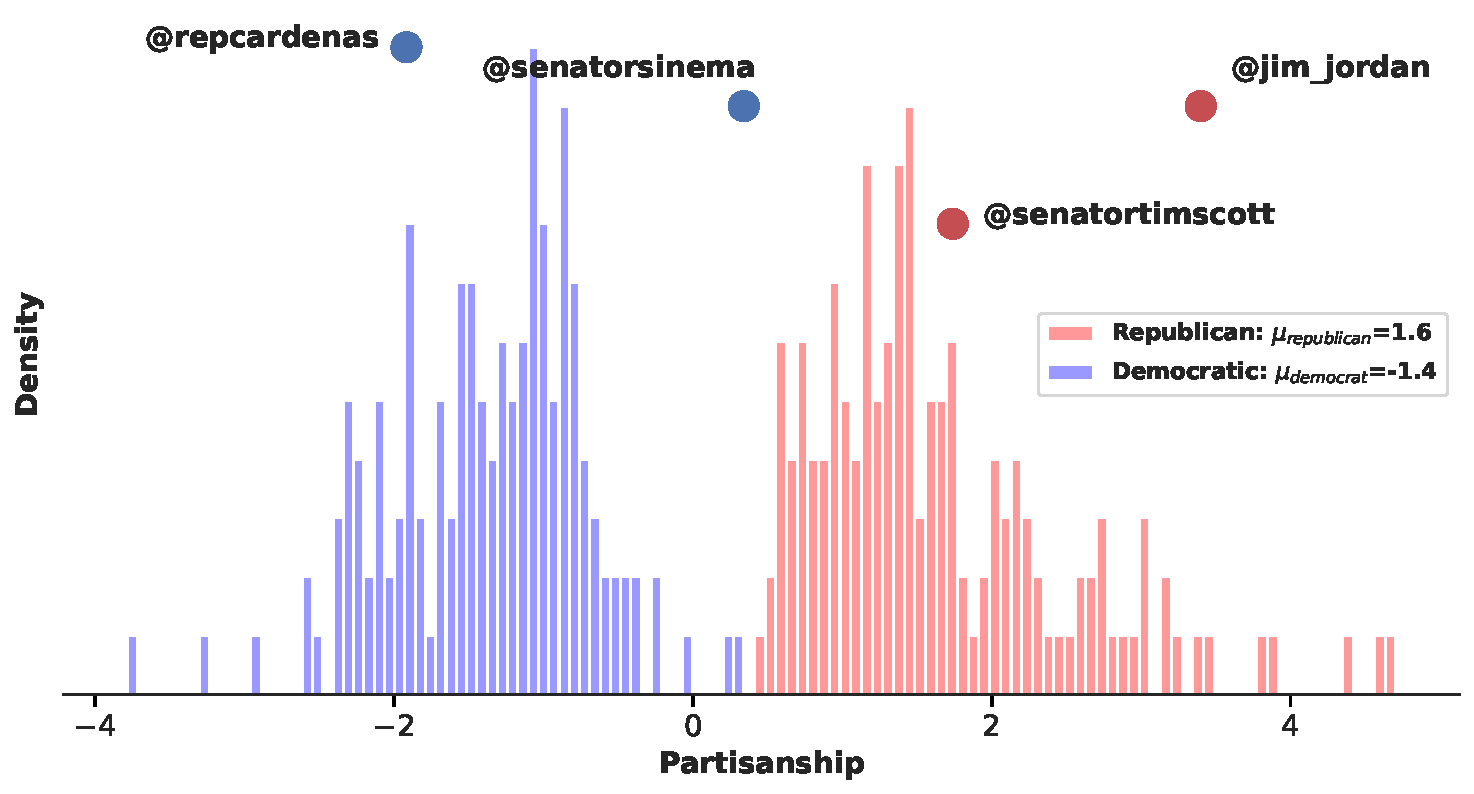
\includegraphics[width=1\columnwidth]{figures/partisanship_us_members-20240424.pdf} 
\end{minipage}
\begin{minipage}[l]{0.47\textwidth}
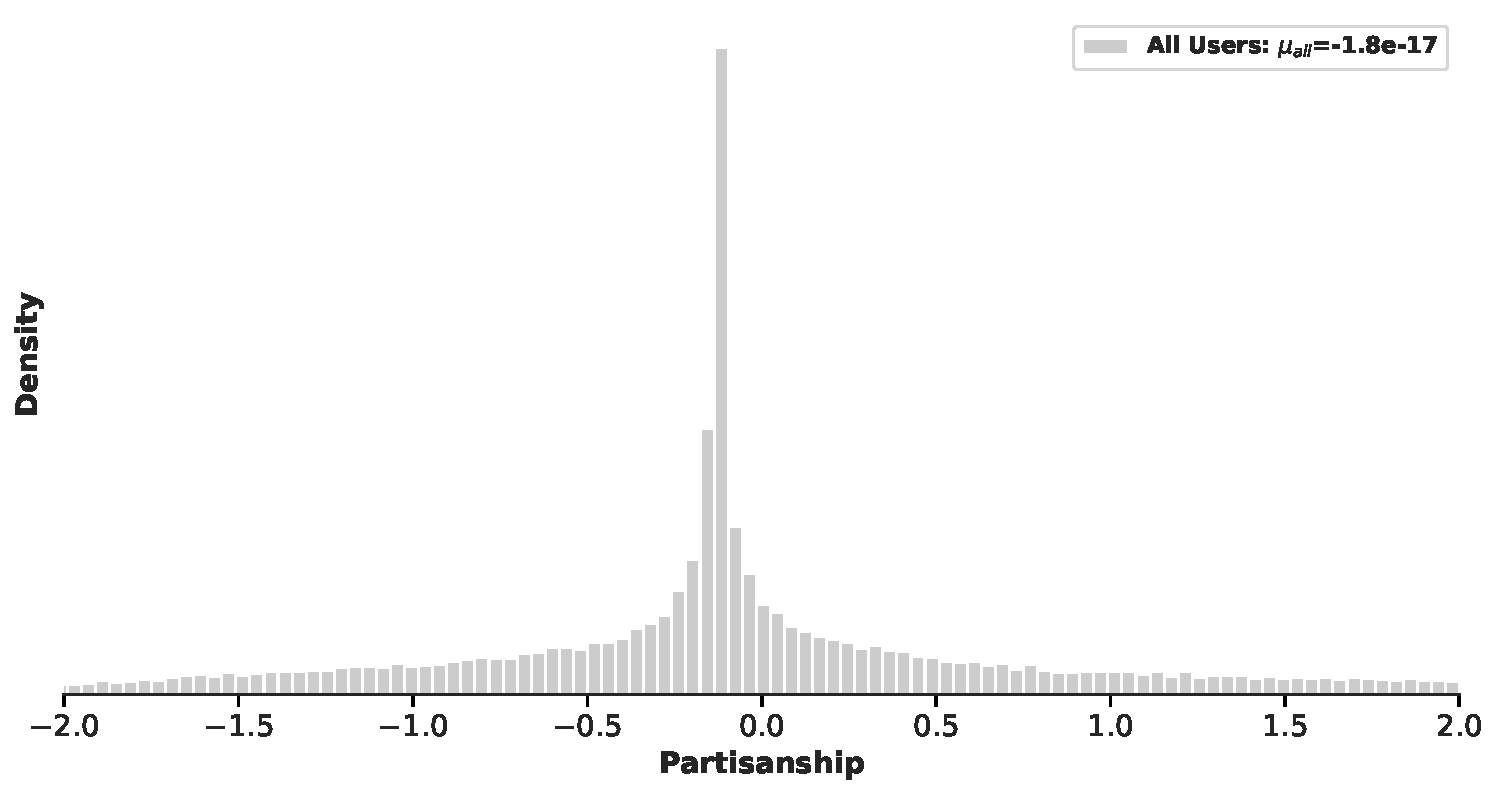
\includegraphics[width=1\columnwidth]{figures/partisanship_all_users-20240424.pdf} 
\end{minipage}

\begin{minipage}[l]{1\textwidth}
\caption{{Estimated Political Orientation of Political Leaders and All Users Using CA}-- We differentiate users' political leanings based on who they follow on Twitter.\label{fig:politican-orientation}}
\end{minipage}

\end{figure}
We note that for our initial set of key political predictive ``followed'' accounts,  we utilize the Twitter accounts of the US House of Representatives and US Senate members from the 117th Congress (2021--2023). In addition to these accounts, we further add another 352~political accounts that were formerly identified by Barber{\'a} {et~al.} (\textit{e.g.,} $@$JoeBiden, $@$VP).\footnote{\url{https://github.com/pablobarbera/twitter_ideology}} Using these accounts, and following the approach as specified by  Barber{\'a}  {et~al.}, we subsequently identified a politically ideological subspace and projected our final list of 43,151 different accounts to this subspace. See Appendix~\ref{sec:appendix-ca} for 
 additional details. As seen in Figure~\ref{fig:politican-orientation}, using this method we manage to obtain a discriminating latent space that allows us to differentiate the ideology of Republican and Democratic political leaders as well as our set of 43,151 accounts. In this setup, the more positive a user's ideology, the more right-leaning; the more negative, the more left-leaning.  

\subsection{Collecting Tweets}
Our dataset initially consisted of 187.6M tweets from 55.4K users that followed our set of key political figures. We collected this data utilizing the Twitter API throughout 2022. We note that following the acquisition of Twitter by Elon Musk, access to the API became restricted limiting our analysis to this time period~\cite{Singh2023}.  Upon identifying these users, given that our work is primarily focused on the US political system, we removed any user that listed their location on their Twitter profile as outside of the United States. To identify US-based users, we utilize the capability of the \texttt{Nominatim} Python tool to geo-code all user's locations based on their Twitter-provided location string and OpenStreetMap.\footnote{\url{https://www.openstreetmap.org/}} Altogether, we remove 12,264 users, leaving us 43,151 users. Upon identifying our user subset, we subsequently utilize \texttt{whatlango}\footnote{\url{https://github.com/abadojack/whatlanggo}} Go library to remove any non-English tweets from our set of users, leaving us 89,599,787 tweets. While we acknowledge several of our users' tweets might have been deleted or taken down by Twitter administrators before we scraped them, this dataset, consisting of over 89.6 million tweets, with an average of 2076.4 (median 614.0) tweets per individual is largely comprehensive of each user's tweeting behavior on the platform.




\subsection{Determining the Toxicity of Tweets\label{sec:labeling-toxic}}

%\subsubsection{Designing an Open-Source Toxicity Classifier}
We design and open-source\footnote{The weights for our model can be downloaded at \url{https://www.github.com/REDACTED}} a contrastive DeBERTa-based~\cite{he2022debertav3} model to determine the toxicity of tweets, later benchmarking our approach on two public datasets and against the Perspective Toxicity API~\cite{perspectiveapi}, the gold standard of toxicity detection~\cite{perspectiveapi,kumar2021designing,rajadesingan2020quick}. We note that throughout our work, we reproduce several results using the Perspective Toxicity classifier and present them in the appendix after obtaining similar results.
To train our new model we rely on the Civil Comments dataset\footnote{\url{https://www.kaggle.com/competitions/jigsaw-unintended-bias-in-toxicity-classification/data}} that was also utilized to train and validate the Perspective API. In addition to utilizing this dataset to augment our trained model, we take two main approaches: (1) data augmentation through realistic adversarial perturbations of the original Civil Comments dataset~\cite{le2022perturbations}, and (2) the inclusion of a contrastive learning embedding layer to help better differentiate toxic and non-toxic texts. For training details of our new model, see Appendix~\ref{sec:app-tox-classifier}.


\vspace{2pt}\noindent
\noindent
\textbf{Benchmarking our Toxicity Classifier.}
Upon training our toxicity model, we compare its performance against the Perspective Toxicity API~\cite{perspectiveapi} and a vanilla finetuned DeBERTa model with a classification head (a two-layer MLP with ReLU activation). To benchmark our toxicity model, we utilize the validation and test dataset of the Civil Comments dataset provided by Google Jigsaw\cite{perspectiveapi} as well as a separate toxicity dataset provided by Kumar {et~al.}~\cite{kumar2021designing}. Kumar  {et~al.}'s datasets consist of 107,620~social media comments (including from Twitter) where each comment was labeled by 5 human annotators as toxic or not (as opposed to the 10 annotators in the Civil Comments dataset). For our $F_1$ score calculations, as in Kumar {et~al.}~\cite{kumar2021designing} and in the Civil Comments dataset, we consider a comment to be toxic if its toxicity $t_i > 0.5$. Again, we utilize this threshold for classifying a comment as toxic, given that this score (as described in the Civil Comments task) indicates that a majority of the Civil Comments annotators would have assigned a ``toxic'' attribute to this comment.

As seen in Table~\ref{tab:benchmark-toxicity}, our contrastive DeBERTa model achieves the lowest mean absolute error (MAE) as well as the highest Pearson correlation and $F_1$ scores across the Civil Comments validation and test dataset. In addition, while obtaining a slightly lower correlation, our model on this separate dataset achieves a lower mean absolute error and a higher $F_1$ score. As such for the rest of this work, when determining the toxicity of tweets, we utilize our contrastive DeBERTa model. We note that our model has a $\rho= 0.870$ Pearson correlation with the scores output by the Perspective API, illustrating its use as an offline alternative with competitive performance to Perspective. Lastly, for this work, as in other works~\cite{hanley2023sub, rajadesingan2020quick}, when determining the overall toxicity of users, or particular groupings of tweets, we utilize the average of the toxicity scores of the tweets output by our model. 
 

\begin{table*}
\centering
\fontsize{8.4pt}{6}
\selectfont
\begin{tabular}{l|ccc|ccc|ccc}
\toprule
& \multicolumn{3}{c|}{\textbf{CC Validation}} & \multicolumn{3}{c|}{\textbf{CC Test }} & \multicolumn{3}{c}{\textbf{Kumar {et~al.} }} \\

Model & MAE & Corr. &Macro-$F_1$ & MAE & Corr. &Macro-$F_1$&  MAE & Corr. &Macro-$F_1$\\ \midrule
DeBERTa & 0.0650 &0.800 &0.841 & 0.0654& 0.797 &0.842 & \textbf{0.241} & 0.383 & 0.539  \\
DeBERTa-contrastive & \textbf{0.0601} &\textbf{0.820} &\textbf{0.851} & \textbf{0.0609}& \textbf{0.818}&\textbf{0.852} & {0.251} & 0.415 & \textbf{0.540}  \\
Perspective API & 0.0961& 0.778& 0.845& 0.0963& 0.777 & 0.842 & 0.332 & \textbf{0.417} & 0.410 \\
\bottomrule
\end{tabular}
\vspace{3pt}
\caption{\label{tab:benchmark-toxicity} Mean absolute error, Pearson correlation, and $F_1$ score of the Perspective API and our DeBERTa models on the Civil Comments Validation and Test dataset. We bold the best scores in each respective column  }
\vspace{-10pt}
\end{table*}




 
\subsection{Topic Analysis with MPNet and DPMeans\label{sec:topic-background}} To later understand how particular types of users interact with different topics composed of toxic tweets, we perform topic analysis on these messages. As found by Grootendorst {et~al.}~\cite{grootendorst2020bertopic,hanley2023partial}, by embedding small messages like Tweets into a shared embedding space and then clustering these embeddings, fine-grained and highly specific topics can be extracted from datasets. To do this, we utilize the large language model MPNet\footnote{\url{https://huggingface.co/sentence-transformers/all-mpnet-base-v2}} fine-tuned on semantic search and a parallelizable minibatch version of the DP-Means algorithm.\footnote{\url{https://github.com/BGU-CS-VIL/pdc-dp-means}}

\vspace{2pt}\noindent
\noindent
\textbf{Fine-tuning MPNet for Topic Analysis.} To compare two tweets' semantic content for later clustering, we rely on a version of the MPNet~\cite{song2020mpnet} large language model that was fine-tuned on semantic search. MPNet maps sentences and paragraphs to a 768-dimensional space, comparing different sentence and paragraph embeddings' semantic content based on cosine similarities (ranging from -1 [highly different] to +1 [highly similar]). We note that the version of MPNet that we utilize was initially fine-tuned on similar social media data (\textit{e.g.}, Reddit comments, and Quora Answers) allowing us to apply this model to our set of tweets. However, to further ensure that our MPNet model is properly suited to our Twitter dataset, as in Hanley et al.~\cite{hhanleyspecious2024}, we further fine-tune this model using an unsupervised contrastive learning objective(\textit{i.e.}, the SimCSE training objective) to better the quality of our embeddings~\cite{gao-etal-2021-simcse}  on our set of tweets. As training data for this fine-tuning, we utilize 1 million tweets randomly sampled from our set of 89.6 million tweets.  See Appendix~\ref{sec:finetune} for additional details. As a reference, we provide two example tweet pairs with similarities at 0.55 and -0.18 in Figure~\ref{figure:paragraph_pairs}. We note that for each tweet within our dataset, before embedding the message, we first remove all URLs, ``@'', ``\#'', emojis, photos, and other non-textual elements from the message. In addition, for each user handle or text hashtag that utilizes camel case (\textit{i.e.}, camelCase) or snake case (\textit{i.e.}, snake\_case), we finally unroll those strings to their constituent elements.


\begin{figure}




\begin{minipage}{1\textwidth}
\hspace{100pt}
\tiny
\textbf{0.735 similarity}
\hspace{120pt}
\tiny
\textbf{-0.032 similarity}
\end{minipage}





\noindent\fcolorbox{black}{lightgray}{%
\begin{minipage}{.44\textwidth}
\tiny
\textbf{Tweet 1:} AZ voters; we need your vote for 
@Adrian\_Fontes and the rest of the Blue ticket. Please, for us, for our children. Please.
\textbf{Tweet 2:} Please vote for 
@Adrian\_Fontes
 and save AZ
\end{minipage}}
\noindent\fcolorbox{black}{lightgray}{%
\begin{minipage}{.44\textwidth}
\tiny
\textbf{Tweet 1:}If a supervisor was giving off those kinds of vibes to a worker in a conventional workplace, an HR complaint would definitely be warranted. Creepy AF


\textbf{Tweet 2:} The close relationship between politics and economics is neither neutral nor coincidental. Large governments evolve through history in order to protect large accumulations of property and wealth.”
\end{minipage}}
\caption{Examples of  Tweet pairs at different similarities (0.735 left and -0.032 right).  }


\label{figure:paragraph_pairs}
\vspace{-10pt}
\end{figure}



\vspace{2pt}\noindent
\noindent
\textbf{DPMeans for Clustering Tweets.}
DP-Means~\cite{dinari2022revisiting} is a non-parametric extension of the K-means clustering algorithm. When running DP-Means, when a given datapoint is a chosen parameter $\lambda$ away from the closest cluster, a new cluster is formed, and that datapoint is assigned to it. This characteristic of DP-Mans enables us to specify how similar individual items must be to one another to be part of the same cluster. Similarly, because DP-Means is non-parametric in terms of the number of clusters formed, we do not need to know \textit{a priori} how many topics are present within our dataset. For additional details about DP-Means, see Appendix~\ref{sec:ap-dpmeans}.

\begin{figure}

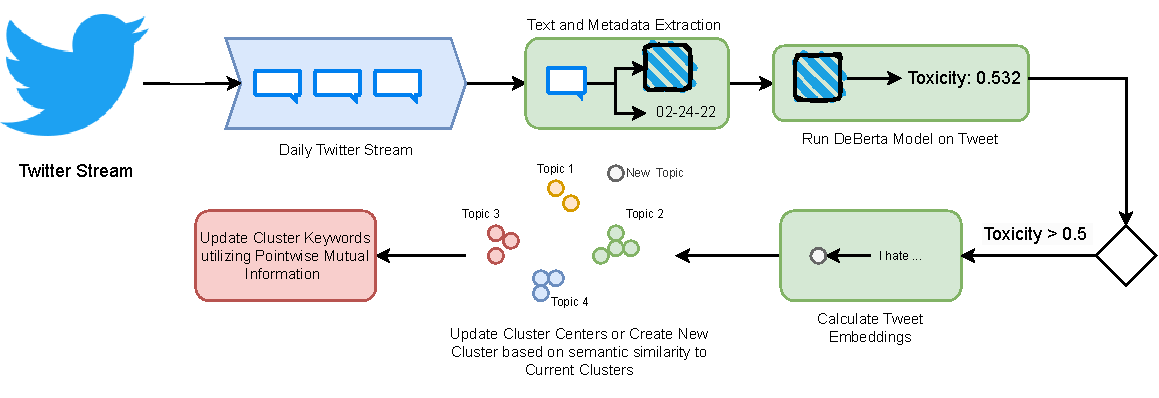
\includegraphics[width=0.9\columnwidth]{figures/Toxic-clustering_documents.drawio.pdf} 
 \caption{Topic analysis of Toxic Tweets---We determine the toxicity, embed, and cluster toxic tweets to identify the most polarized and toxic conversations on Twitter throughout 2022. We note that for this approach, we limit our analysis to English tweets. We utilize the \texttt{whatlango} Go library to determine the language of tweets. \label{fig:toxic-cluster}}
\end{figure}


\vspace{2pt}\noindent
\noindent
\textbf{Topic Analysis Pipeline.}
Having outlined the constituent elements of our topic analysis algorithm, we now go over the full topic analysis pipeline (Figure~\ref{fig:toxic-cluster}): Throughout 2022, as we gathered the tweets of our set of 43,151 Twitter users, using our DeBERTa-contrastive model, we identify potentially toxic tweets (\textit{i.e.}, toxicity $t_i$ > 0.50). Following the identification of these potentially toxic tweets and separating out non-English tweets with \texttt{whatlango}, using MPNet, we subsequently map these tweets to a shared embedding space. Finally, we continuously cluster these tweets to identify topics amongst these toxic tweets using the DP-Means algorithm. To make these clusters that represent topics amongst our set of tweets, human-understand we employ two different approaches. First, we designate the tweets closest (\textit{i.e.}, with the largest cosine similarity) to the center of the cluster as the ``representative tweet'' of the cluster~\cite{grootendorst2020bertopic}. Second, we determine the most distinctive keywords of each cluster using pointwise mutual information~\cite{bouma2009normalized} (detailed in Appendix~\ref{sec:pmi}). In this way, after clustering our set of tweets, we can later extract the semantic meaning of the various clusters outputted. 

As recommended by Hanley {et~al.} we utilize a $\lambda$ of 0.60 for our clusters (precision near 0.989 for MPNet~\cite{hanley2022happenstance,grootendorst2020bertopic}). Finally, we extract keywords from these clusters using the pointwise mutual information metric and determine the most representative tweets by determining the tweet with the highest cosine similarity to the cluster center. Altogether, across the 5,509,042~English-language toxic tweets from our set of 43,151~Twitter users, we identified 5,288~clusters with at least 50~toxic tweets. 

\subsection{Generalized Additive Models}
Throughout this work, we utilize Generalized Additive Models (GAM)~\cite{hastie2017generalized} to determine the relationships between our variables of interest (\textit{e.g.}, user partisanship, and user toxicity). For GAMs, the relationship between the independent and dependent variables is not assumed to be linear but is rather estimated as a smooth regularized nonparametric function. Namely, given a dependent variable $Y$ and a set of $p$ independent variables  $X$, GAM's are estimated as:
\begin{equation}
    g(E(Y))=\alpha+s_1(x_1)+\cdots+s_p(x_p),
\end{equation} where $g()$ is a linking function that connects the expected value of the dependent variable $Y$ to values of functions $s_i()$ of independent independent variables in $X$. For example, when estimating probabilities the logit function is often utilized as with ordinary Generalized Linear Models~\cite{demaris1992logit}. The functions $s_i()$ represent smooth nonparametric functions of the variables in $X$ that are fully determined by the data in $X$ rather than by a parametric function. For GAMs, these $s_i()$ are estimated simultaneously, and the estimated value of $g(E(Y))$ is determined by implying adding up the values of the $s_i()$ functions. Throughout this work, we utilize the Python \texttt{Pygam} library to fit our regressions and utilize the Generalized Cross Validation Loss Criteria (GCV)~\cite{demaris1992logit} for estimating the $s_i()$ functions when fitting. The Generalized Cross-Validation Loss Criteria takes a LOOCV (Leave One Out Cross-Validation) approach to fitting smoothers on the data in X. 

Utilizing GAMS versus other more traditional models allows us  (1) to not assume linear relationships between our dependent and independent variables, and (2) to have better interpretability given that the partial contribution of a given variable $x_i$ to determining the value of the dependent variable Y is a function only of its corresponding function $s_i()$. 

\subsection{Ethical Considerations} 
Within this work, we largely focus on identifying large-scale trends in how different Twitter interact with one another. While we do calculate toxicity and polarization levels for individual users, we only display the names of verified public users or users with more than 500K followers, redacting the names of all other accounts. 
We lastly note that our Twitter data was largely collected before Elon Musk's private acquisition of Twitter on October 27, 2022, and all of our data was collected before the later restrictions placed on the collection of tweets on June 30, 2023.\footnote{\url{https://help.twitter.com/en/rules-and-policies/twitter-limits}}



\section{RQ1:  User-Level Factors in Toxicity on Twitter\label{sec:toxic_middle}}
Having provided background on our methodology and dataset, in this section, we discuss several of the user-level factors that coincide with and contribute to the toxicity on Twitter. 


\subsection{Setup}
Here, we examine the role of several user-level factors in contributing to or affecting the rate at which individual users are toxic on Twitter. Specifically, we examine the following user characteristics in contributing to or mitigating the toxicity of individual users on Twitter: 

\begin{enumerate}

\item \emph{The verified status of the account}
\item \emph{The number of years the account has been active on Twitter}
\item \emph{The log of the number of the account's followers}
\item \emph{The log of the number of accounts the user follows}
\item \emph{The account's partisanship as determined by our Correspondence Analysis}
\item \emph{The estimated average toxicity of all users the account mentioned/@ed on Twitter (\textit{i.e.}, accounts that the user has interacted with)}
\item  \emph{The estimated average partisanship of the accounts the user mentioned/@ed}
\item \emph{The standard deviation of the partisanship of the accounts that the user mentioned (\textit{i.e.}, the range of political views with which the user interacts)}
\item \emph{The average value of the partisanship of all accounts the user mentioned/@ed}
\item \emph{The average difference in the partisanship of the account the given user mentioned/@ed and the users's partisanship}



\end{enumerate}

\noindent We fit these ten covariates against each of our account's average toxicity scores. As in past studies, we fit against the verified status, the age of the account, and the information about the activity of the accounts (\textit{e.g.}, the number of followers and the number of users followed)  to understand how general account characteristics that the Twitter API returns correspond with user toxicity~\cite{hua2020characterizing, chatzakou2017measuring}. As shown in prior work, the verification status, the number of years active, and levels of activity, depending on the context, can have differing effects on the adversarial nature and toxicity of Twitter accounts~\cite{chatzakou2017measuring,ribeiro2018characterizing}. Similarly, as shown in Saveski et al.~\cite{saveski2021structure} and Kraut et al~\cite{kraut2010dealing}  many individual-level characteristics are predictive of users' toxicity as it predicts their level of familiarity with a given platform and their tendency to break norms (\textit{e.g.}, post toxic content).  Thus, as a baseline, and to help ground our study, and determine how these account characteristics correlate with increased toxicity within the context of politically US-aligned account interactions, we include them in our model. In addition to these basic account attributes, we include information about each Twitter account's partisanship on the US left-right political spectrum as well as information about how that Twitter user interacts with other US politically aligned Twitter accounts~\cite{marozzo2018analyzing}. These variables' inclusion allows us to answer our research question about whether and how affective polarization and partisanship affect the toxicity of individual accounts~\cite{kubin2021role}.


\begin{figure}
\begin{minipage}[l]{1.0\textwidth}
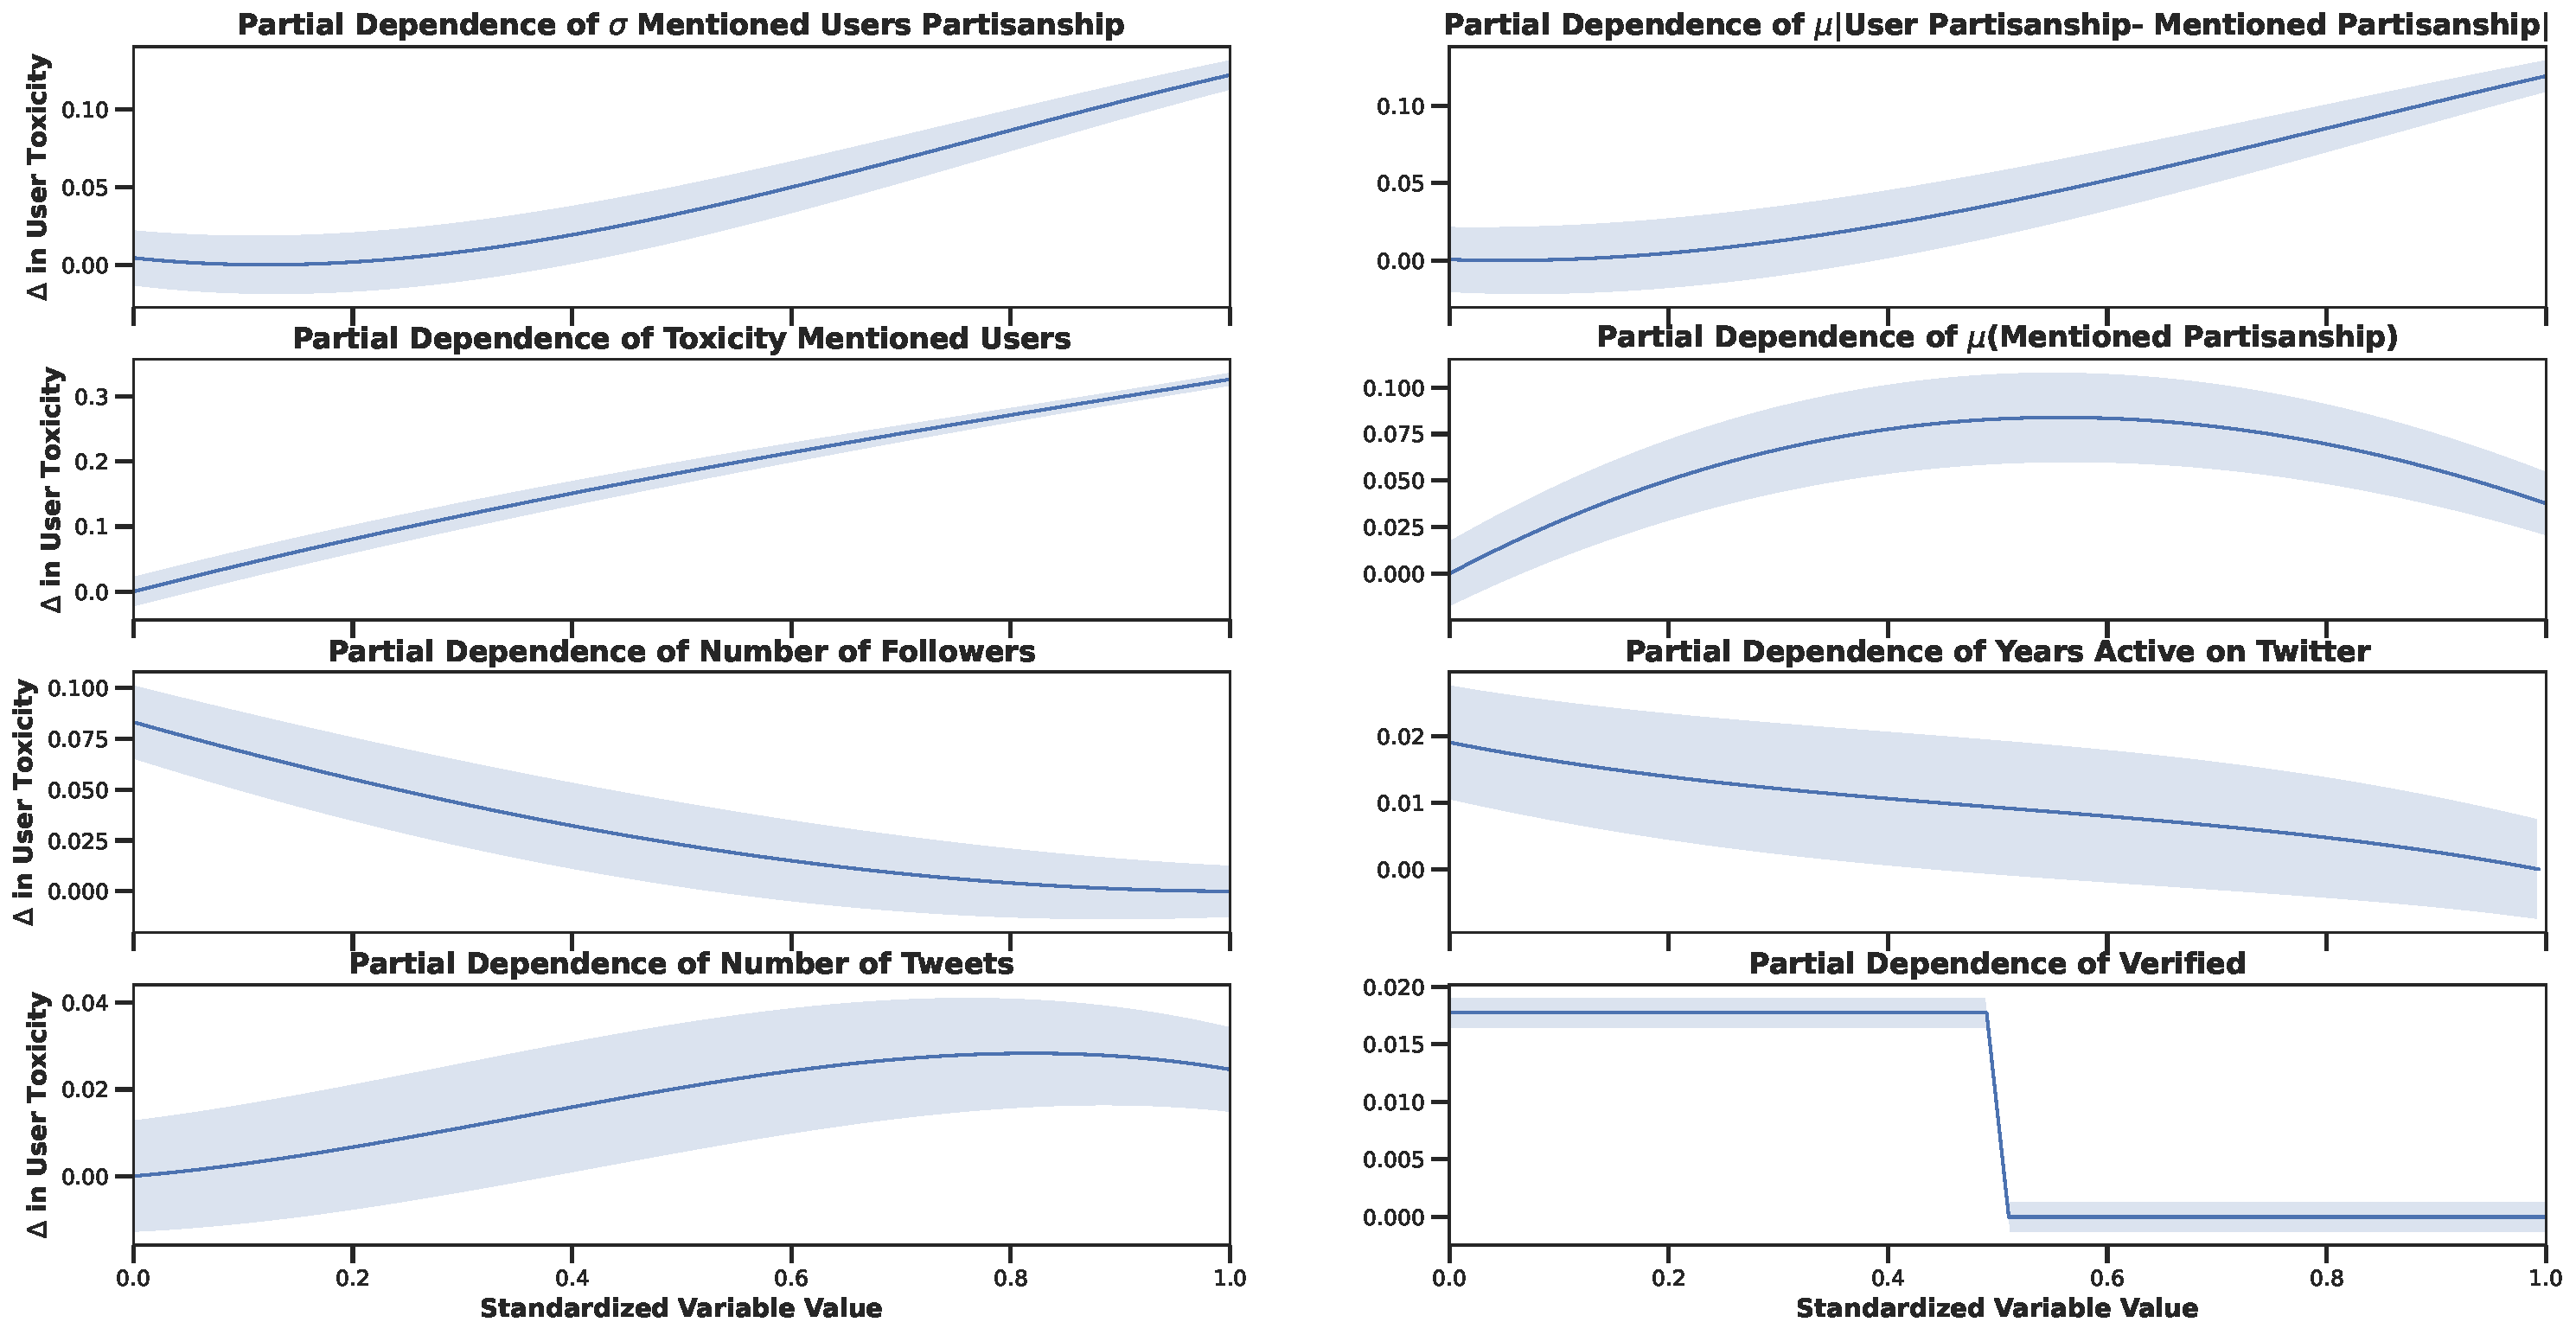
\includegraphics[width=1\columnwidth]{figures/partial_dependence_important_variables.pdf} 
\end{minipage}
\begin{minipage}[l]{1\textwidth}
\caption{Partial dependencies with 95\% Normal Confidence intervals between our fitted standardized dependent variables and user toxicity.}
\label{fig:partial-dependence-user-toxcity}
\end{minipage}

\end{figure}

\begin{table}
    \small
    \centering
    \begin{tabularx}{0.90\columnwidth}{l|rrr}
    Train $R^2$:  0.239 ,   $R^2$:  0.207  \\
    \toprule
      Dependent Variable  & Pearson Corr. $\rho$ & Kendall's $\tau$  & Permut Import. \\    \midrule
  Verified Status & ---- &-0.242 & 0.053  \\
  Years Active on Twitter & -0.197& -0.147 & 0.027 \\
  Log \# Followers & -0.206 &-0.122 & 0.205  \\
  Log \# Followed & -0.135 & -0.090 & --- \\
  Log \# Tweets in 2022 & 0.147 & 0.200  & 0.045\\
  Toxicity of Mentioned Users& 0.318& 0.362 & 0.374 \\
  partisanship  &0.054& 0.061 & --- \\
  $\sigma$(Mentioned partisanship)&0.317& 0.332	& 0.150\\
   $\mu$(Mentioned partisanship) & 0.110 &0.099 & 0.067  \\
  $\mu$|User partisanship- Mentioned partisanship|&0.287& 0.283 & 0.080\\


    
    \bottomrule
     %\multicolumn{2}{c}{ $^\ast p<0.05; \;  ^{**} p<0.01; \; ^{***}p<0.001$ }
    \end{tabularx}
  \caption{Pearson correlation $\rho$ and Kendall's $\tau$, and permutation importance of dependent variables and user's toxicity. As seen in the above table, a user's interaction with a wide political variety of users and interacting with other users with higher toxicity correlates with a given user's toxicity. } 
   \vspace{-15pt}
   \label{table:importance-user-toxicity}
\end{table}





To understand how these factors interact with and contribute to toxicity on Twitter, we fit a Generalized Additive Model (GAM) on the average toxicity score of users (Table~\ref{table:importance-user-toxicity}). When fitting our model, we perform variable selection using forward selection based on the Akaike Information Criterion~\cite{akaike2011akaike}, which ended up eliminating the number of followed accounts as well as the user partisanship as variables from our final model. Furthermore, to ensure that our model generalizes, we further reserve 10\% of our data as validation, and in our results report our model's $R^2$ value on this validation set. Finally, after fitting this regression, we further determine the estimated importance of each variable to our final model by permuting the features and seeing the estimated impact on the $R^2$ score on the validation set of our data (permutation importance is a widely used statistic for determining the relative information of features to models~\cite{altmann2010permutation}). We present the partial dependence (with 95\% Normal confidence intervals) on the user toxicity of each independent variable in Figure~\ref{fig:partial-dependence-user-toxcity} and present Pearson correlation, Kendall's $\tau$  (a more robust version of the Spearman Correlation), and each independent variable's permutation importance in Table~\ref{table:importance-user-toxicity}.  Our final model achieved a $R^2$ value of 0.239 on our training data and a $R^2$ value of 0.207 on our validation dataset, illustrating that our model does generalize to users outside of its training data.


We lastly note that to ensure the robustness of our approach, we separately perform the same analysis utilizing the toxicity scores output by the Perspective API, obtaining similar results. We present these results in Appendix~\ref{sec:perspective-user-app}.

\subsection{Baseline Account Characteristics}
We first provide an overview of how several baseline account characteristics contribute to the toxicity of each user. As seen in Table~\ref{table:importance-user-toxicity}, we do indeed observe that each of the user characteristics that we consider (to varying degrees) \emph{does} indeed have observed a correlational effect on how toxic users' tweets tend to be. We consider each of these effects below.

\vspace{2pt}\noindent
\noindent
\textbf{Verified Status.} As seen in Table~\ref{table:importance-user-toxicity} and Figure~\ref{fig:partial-dependence-user-toxcity}, as also found by Hua {et~al.}~\cite{hua2020characterizing}, whether a user is verified has a modest effect on how often they post toxic tweets, with verified users being less likely to tweet harmful or toxic messages compared to non-verified users. Overall, we find that a user's verification status has a Kendall's $\tau$ of -0.242 with their verification status and has a permutation importance of 0.053 in our final model. This suggests that when users become verified and their account is associated with their offline life, users tend to be less toxic. We note that we collected users' verification status before the implementation of Twitter Blue (users could pay 8 USD to become verified) in November 2022~\cite{Fung2023}.

\vspace{2pt}\noindent
\noindent
\textbf{Years Active on Twitter.} As users stay on Twitter, as seen in Figure~\ref{fig:partial-dependence-user-toxcity}, we observe that they are less likely to be toxic. As argued by Rajadesingan {et~al.}~\cite{rajadesingan2020quick} in their paper on Reddit, as social media users stay longer on particular platforms and adjust to interacting with other users, they tend to be less aggressive and toxic with other users. We see a similar result here, with older users being less toxic than younger ones. Overall, we observe that the number of years that a user is active on Twitter has a Pearson correlation of $\rho=-0.197$ with their average toxicity and a permutation importance of 0.027. This accords with past research that has found that news users, who are used to the social mores and norms of a given online community, may more frequently violate those norms and post toxic content~\cite{kraut2010dealing}.

\vspace{2pt}\noindent
\noindent
\textbf{Number of Followers.} Like verified status, and as argued by Marwick {et~al.}~\cite{marwick2011see}, extremely popular users are less likely overall to be toxic than users with smaller followings. These users, often create friendly public personas to interact with their followers, rarely attacking other users or posting toxic content. As seen in Figure~\ref{fig:partial-dependence-user-toxcity}, we see the same: more popular users that have more followers are less likely to post toxic tweets ($\rho=-0.206$). This variable has a permutation importance of 0.205 suggesting the high relative importance in determining the toxicity of accounts. 

%spam and fake accounts~\cite{Fishkin2022}, having an unusually small number of followers is often an indicator of a fake account. Similarly,
\vspace{2pt}\noindent
\noindent
\textbf{Number of Tweets.}
Many accounts in our Twitter dataset post several times a day, with the median account posting 614.0~times throughout 2022, and one account posting 413,658 times. As seen in Figure~\ref{fig:partial-dependence-user-toxcity} with a permutation importance of 0.045 and a Pearson correlation of $\rho=0.147$, we observe that as Twitter users post more, generally their average toxicity increases. This finding reinforces past work that suggests that accounts that post excessively and that spam Twitter, are more likely to be toxic~\cite{salehabadi2022user}. %This variable has a permutation importance of 0.045 

%Altogether, the number of tweets posted accounts for 0.75\% of the variability in user toxicity.

\begin{figure}
\begin{minipage}[l]{0.6\textwidth}
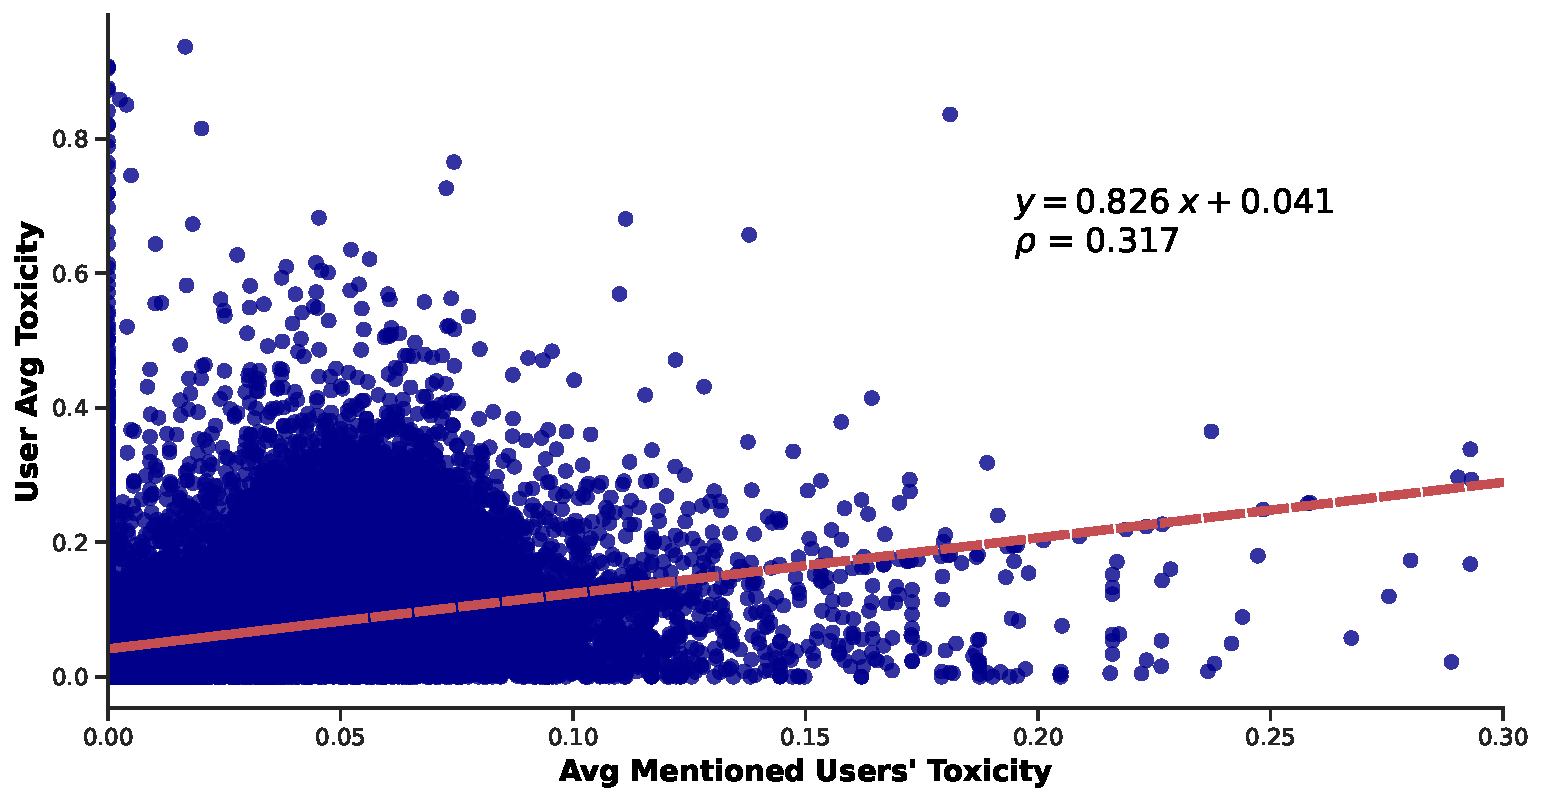
\includegraphics[width=1\columnwidth]{figures/toxicity_vs_mentioned_toxicity-20240424.pdf} 
\end{minipage}
\begin{minipage}{.33\textwidth}
  \centering
  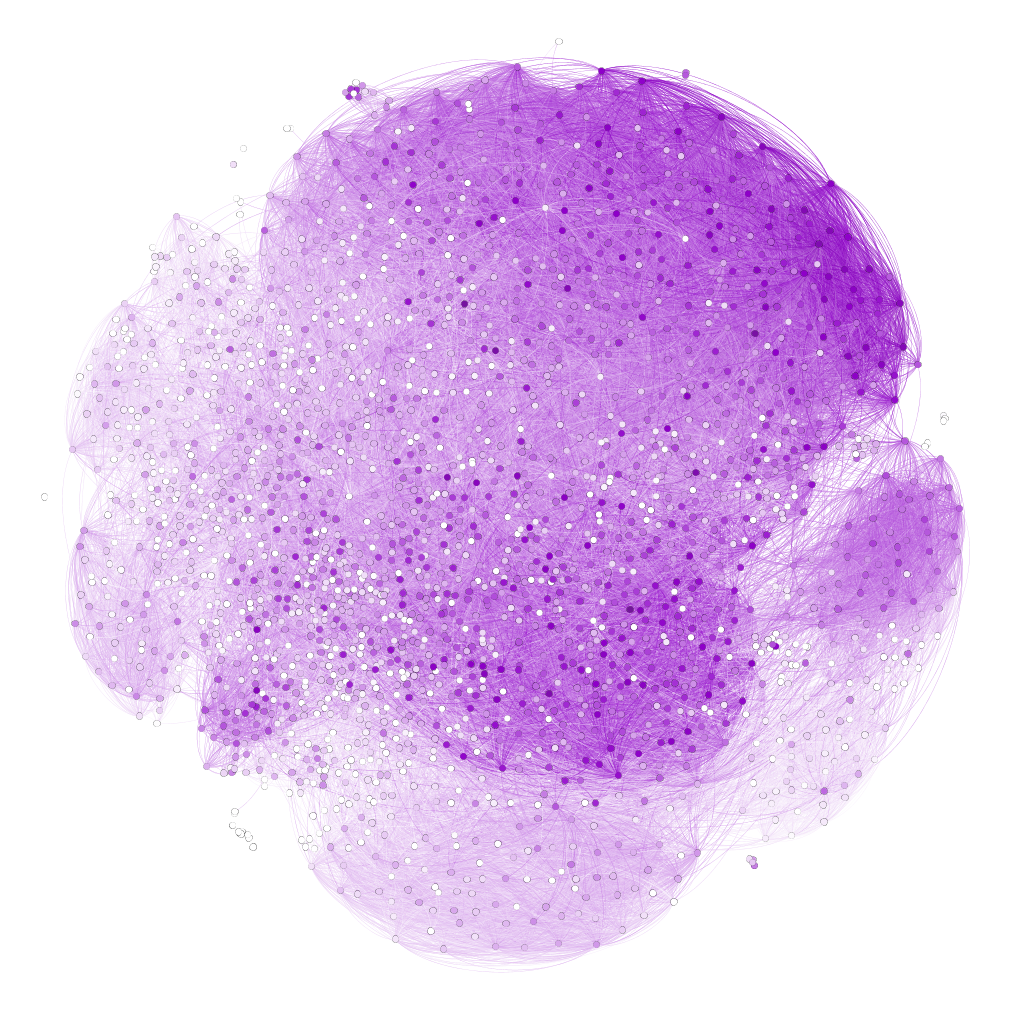
\includegraphics[width=1\linewidth]{figures/toxicity-graph.png}
  \label{fig:Twitter-reddit-toxicity-time}
\end{minipage}
\begin{minipage}[l]{1\textwidth}
\caption{The more toxic the users mentioned by a given user, on average, the more toxic the content of that particular user. Within the mention graph (the darker the purple the more toxic) of user interactions, toxicity has an assortativity coefficient of 0.071, suggesting that, to some degree, users who post toxic content have a slight tendency to mention and interact with other users who post toxic content. \label{fig:toxicity-vs-mention}}
\end{minipage}

\end{figure}

\subsection{Calculated Account Characteristics: Toxicity and Political Orientation\label{sec:calculated}}

Here we provide an overview of how the different political and toxicity measures that we calculated contribute to individual user-level toxicity. 

\vspace{2pt}\noindent
\noindent
\textbf{Toxicity of Mentioned Users.} We find that as users interact with or mention (@ing) other users who post toxic content, they themselves are more likely to be toxic. As seen in Figure~\ref{fig:partial-dependence-user-toxcity}, the average toxicity of accounts with which a user interacts has a nearly linear relationship with the user's own toxicity with very little variation. Indeed, we find this variable to be the most important in determining a user's toxicity, with it having a permutation importance of 0.374 and a Pearson correlation $\rho=0.318$. The most important of our covariates in terms of explainability, this result reinforces many prior findings about when and why particular users are toxic online~\cite{saveski2021structure,rajadesingan2020quick}. Creating a mention (@) graph among our 43,151~users and plotting users' toxicity against the toxicity of their mentioned accounts in Figure~\ref{fig:toxicity-vs-mention}, we further find some degree of assortativity based on toxicity (0.071), with more toxic users more likely to interact with each other than with non-toxic users, supporting this result. 


\begin{figure}
\begin{minipage}{.33\textwidth}
  \centering
  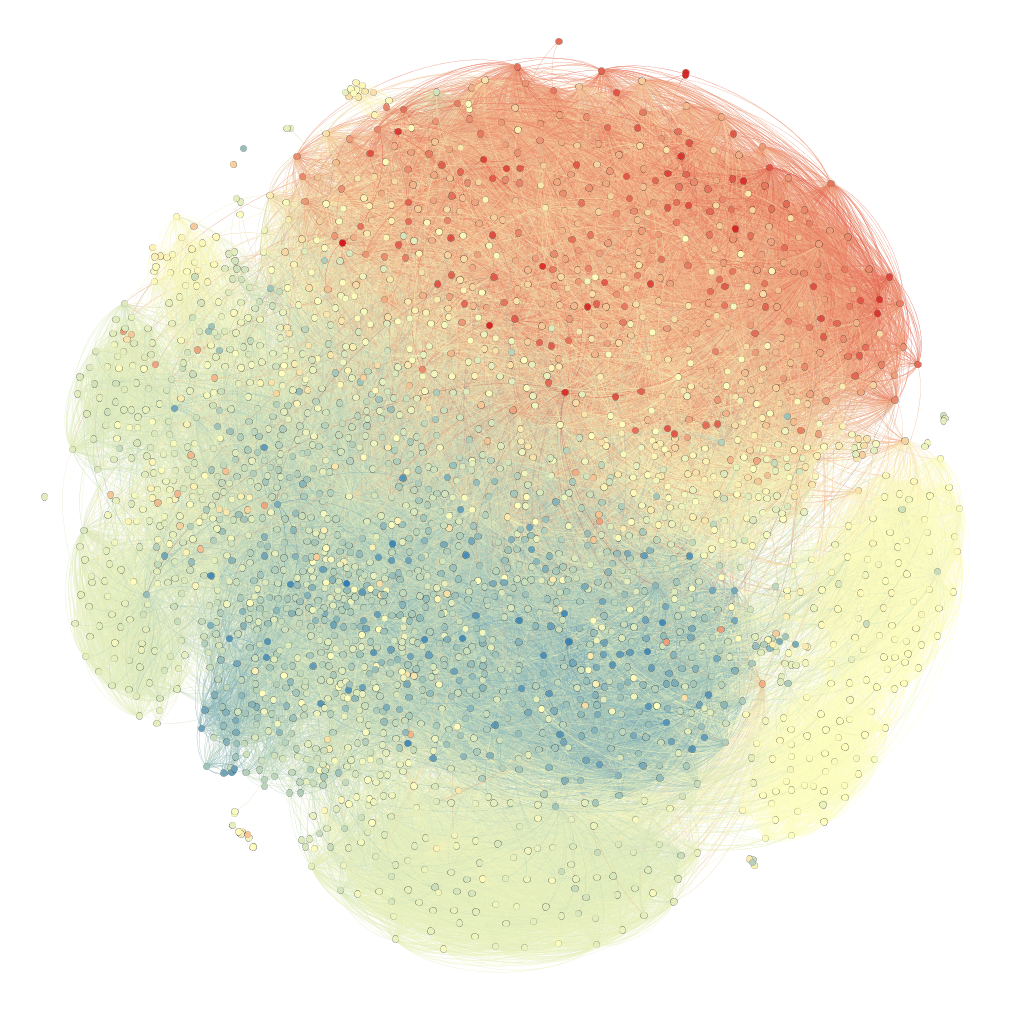
\includegraphics[width=1\linewidth]{figures/republican-democratic-graph.png}
\label{fig:twitter-reddit-partisanship-time}
\end{minipage}%
\begin{minipage}{.6\textwidth}
  \centering
  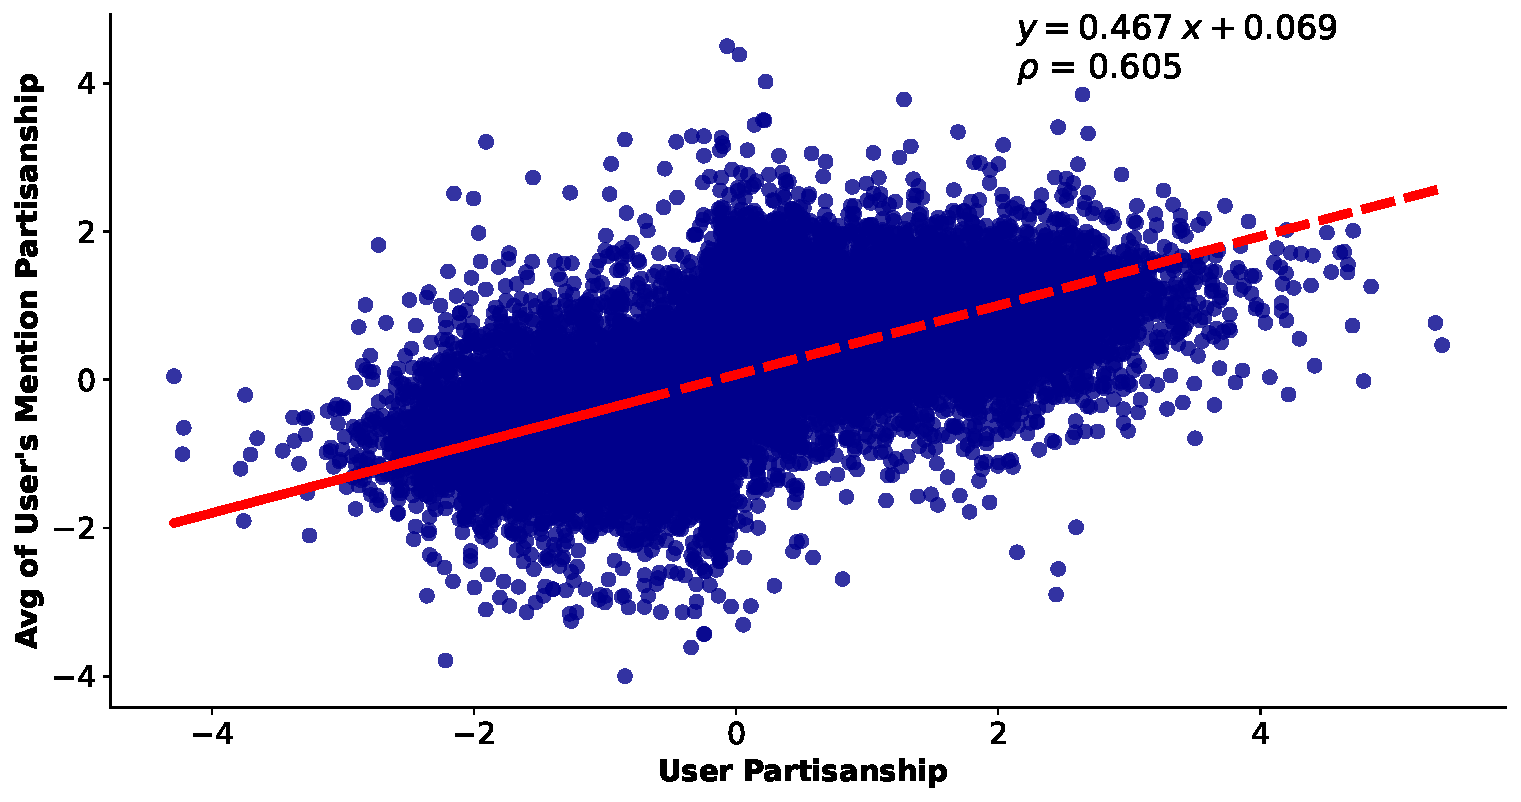
\includegraphics[width=1\linewidth]{figures/ideology_vs_avg_mention-20240429.pdf}
\label{fig:twitter-reddit-partisanship-time2}
\end{minipage}%

\begin{minipage}{1\textwidth}
\caption{Within the mention graph of user interactions (red/right-leaning and blue/left-leaning), partisanship has an assortativity coefficient of 0.266, suggesting that conservative users mention and interact more with right-leaning users while liberal users interact more with and mention other left-leaning users. Similarly, graphing the average of each user's mention's partisanship against their own partisanship, we find significant assortativity (Pearson correlation $\rho=0.605$)\label{fig:graph-of-political-interactions}
}
\end{minipage}

\end{figure}
\vspace{2pt}\noindent
\noindent
\textbf{Partisanship of Mentioned Users.} As the average value of the partisanship increases (the mentioned accounts become more right-wing), we find that the average toxicity of an account increases (Figure~\ref{fig:partial-dependence-user-toxcity}) before decreasing again on the right side of the political spectrum. We thus find that when users mention users on the political extreme, this does not indicate increased toxicity; rather we find in general that users who reference these users tend to tweet less toxic content on Twitter. This may do with the tendency that the users who reference these politically polarized/extreme users also tend to be near the political extremes themselves. Creating a mention/@  graph among our 43,151~users, we find a moderate degree of assortativity (0.266), thus finding that users, on the whole, tend to interact with other users of similar political views (Figure~\ref{fig:graph-of-political-interactions}) and that this tendency is not necessarily correlated with increased toxicity.  Graphing the average partisanship of a user's mention against their own partisanship we further observe a high assortativity (Pearson correlation of $\rho=0.605$). 
\begin{figure}
\begin{minipage}[l]{0.48\textwidth}
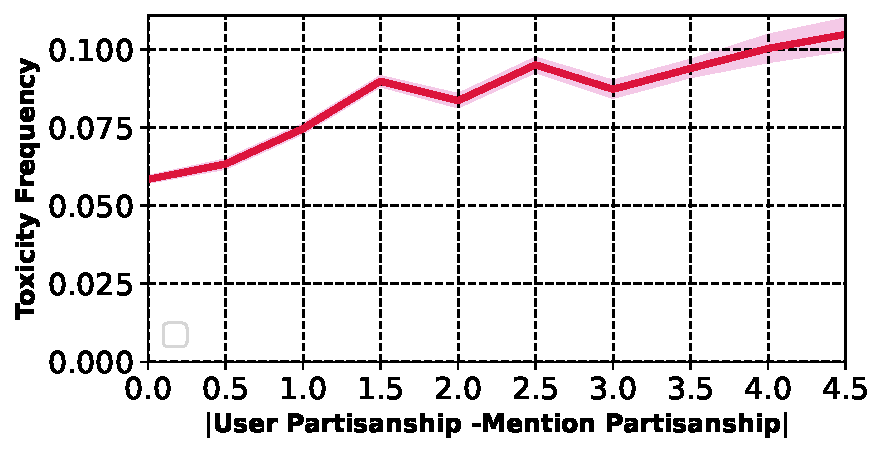
\includegraphics[width=1\columnwidth]{figures/toxicity_vs_mention-20240428.pdf}
\end{minipage}
\begin{minipage}[l]{0.33\textwidth}
\caption{As the difference in the partisanship of users and those that they mention/@ increases, the probability of users tweeting toxicly increases. 95\% Normal Confidence Intervals.
\label{fig:toxicity_vs_mention-new}}
\end{minipage}
\end{figure}

Instead, as was seen in (Figure~\ref{fig:partial-dependence-user-toxcity}) it is the difference in partisanship between a user and their mentions that linearly determines the toxicity of users. The average difference in the partisanship between a user and their mentioned accounts has a $\rho = 0.287$ Pearson correlation with the user's own toxicity and has a permutation importance of 0.080. Indeed, as seen in Figure~\ref{fig:toxicity_vs_mention-new}, we observe across our entire dataset that as the difference between a user's partisanship and the partisanship of the corresponding user that mention/@ increases the probability that they tweet toxicly increases. This illustrates, as found elsewhere~\cite{hanley2023sub,mamakos2023social}, that as users interact with more users different in partisanship than themselves, they are more likely to be toxic.  As an example a left-wing user (-1.53) with a particularly high standard deviation for the diversity of their mentions (1.818), often engaging in heated discussion with right-wing and left-wing accounts wrote the tweet concerning the former Republican US president Donald Trump:
\begin{displayquote}
\small
\textit{
This is so indescribably fucked up. Except I love Nancy Pelosi giving him the shiv.}
\end{displayquote}
\noindent
Similarly, a different  left-wing account (-1.504), which also regularly interacts with right-wing and left-wing accounts (1.65), regarding former Republican US president Donald Trump's son wrote:
\begin{displayquote}
\small
\textit{
Fuck him. No, seriously, fuck him. If anyone’s a welfare queen it’s him...}
\end{displayquote}
\noindent


\begin{figure}
\begin{minipage}[l]{0.48\textwidth}
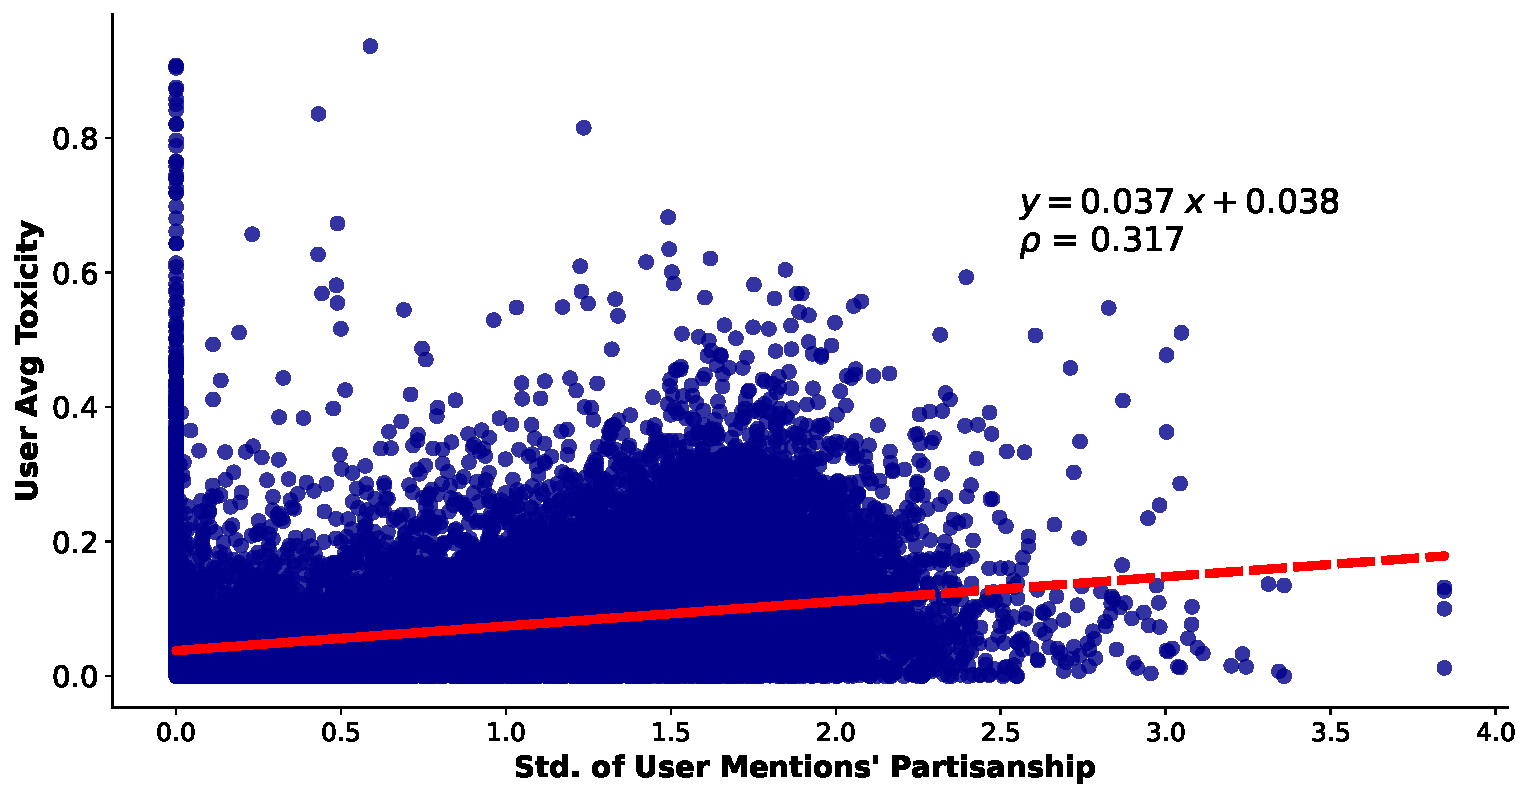
\includegraphics[width=1\columnwidth]{figures/toxicity_vs_avg_mention-20240429.pdf}
\end{minipage}
\begin{minipage}[l]{0.33\textwidth}
\caption{As users mention a wider range of users along the political spectrum they are more likely to tweet toxic messages. 
\label{fig:politican-variance-toxicity2}}
\end{minipage}
\end{figure}


\vspace{2pt}\noindent
\noindent
\textbf{The Political Diversity of Mentions.}
In addition to finding that as users interact with more users different than themselves, from Figure~\ref{fig:partial-dependence-user-toxcity} and Table~\ref{table:importance-user-toxicity}, we find that as users mention/@ a wider political diversity of users, the more toxic their own tweets. With a Pearson correlation of $\rho =0.317$ and a permutation importance of  0.15, we see that this feature is relatively important in our fit model with it heavily contributing to the prediction of a user's toxicity (Figure~\ref{fig:politican-variance-toxicity2}).  This reinforces the finding of Mamakos et~al.~\cite{mamakos2023social}. who also found that when users engage with both left-leaning and right-leaning accounts on Reddit, they are more likely to engage in toxic behaviors on the platform. 


%We thus see these accounts which often engage with a wide diversity and with users that are different from themselves, often tweet toxically sometimes concerning their political opponents.  







\subsection{Summary}
In this section, using a GAM, we explored the role that several user-level characteristics have on the rate of user toxicity on Twitter. We find, most importantly, that users who interact and mention other users who regularly post toxic content are more likely to be toxic themselves. Similarly, we found the more a given user interacts with a politically diverse set of accounts, the more likely that account is to tweet toxic content. We replicate these results with the Perspective API in Appendix~\ref{sec:perspective-user-app} getting similar results. 

\section{Factors and Changes in Polarized and Toxic Topics on Twitter}
Having investigated the role that various user characteristics have in user toxicity on Twitter, we now explore how different characteristics affect different negative and toxic topics on Twitter. Specifically, how does the toxicity of topics on Twitter change based on the makeup of the user participating in these conversations? First discussing and performing some qualitative analysis on the most toxic and political ideological conversations on Twitter, we then determine how the political views, the diversity of political views, and the overall toxicity of the users participating in given conversations affected particular topics discussed in 2022.

\subsection{Setup}
In this section, we utilize a combination of MPNet and DP-Means as specified in Section~\ref{sec:topic-background} to perform topic analysis on the English language tweets within our dataset. After running our algorithm on the 5.5M~toxic tweets from our set of 43.1K~Twitter users, we identified 5,288~clusters with at least 50~toxic tweets. Upon identifying these clusters, as outlined in Section~\ref{sec:topic-background}, we further extract the most characteristic (often offensive) words within each cluster as well as each cluster's most representative toxic tweet. Before further detailing some of the characteristics of each of these toxic tweet clusters, we now give a brief overview of how we estimate the overall toxicity and political bend of each particular topic after identifying their corresponding cluster of toxic tweets.

\begin{figure}
\begin{subfigure}[l]{0.45\textwidth}
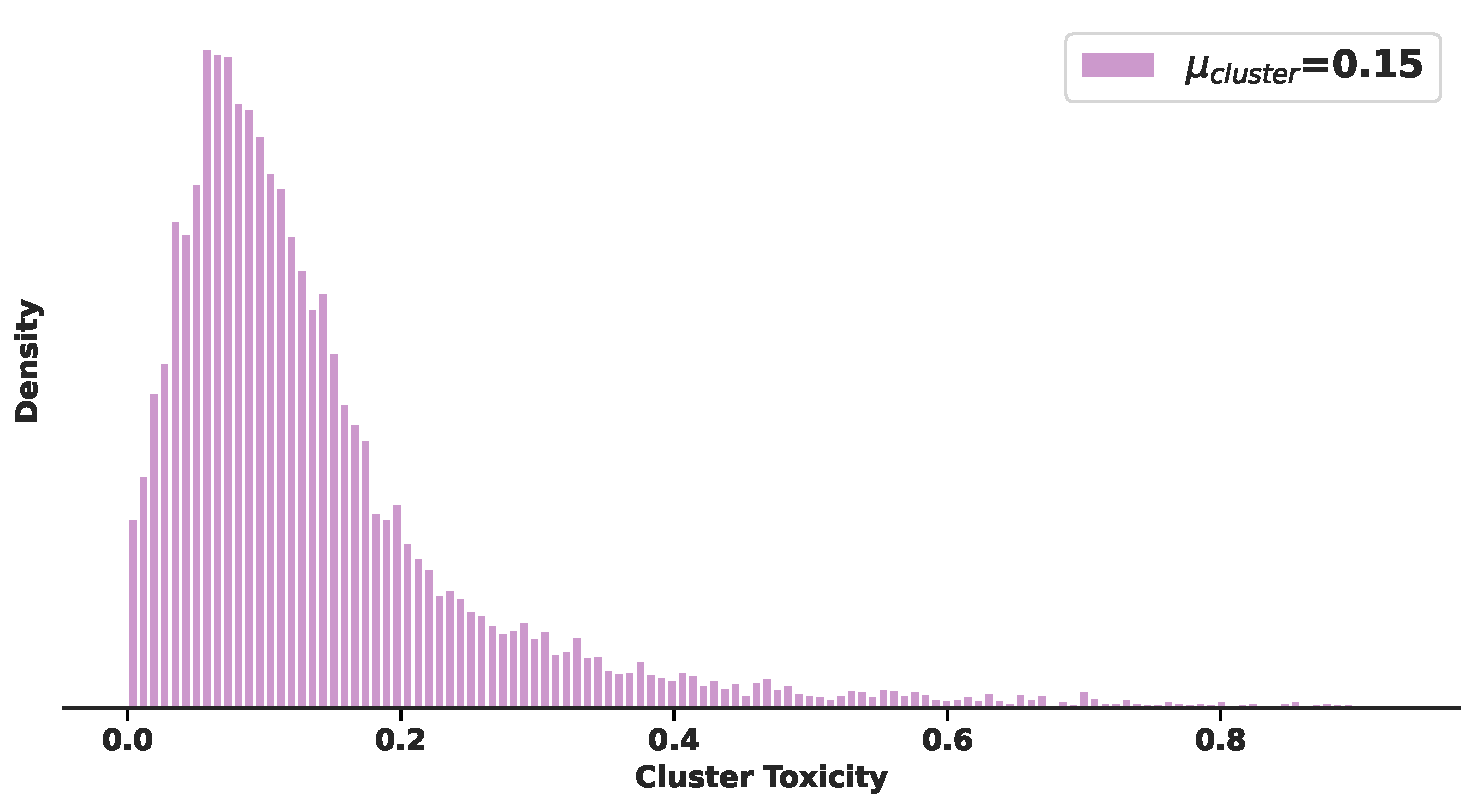
\includegraphics[width=1\columnwidth]{figures/cluster_toxicity_dist3.pdf}
\caption{}
\label{fig:cluster-dists-toxic}
\end{subfigure}
\begin{subfigure}[l]{0.45\textwidth}
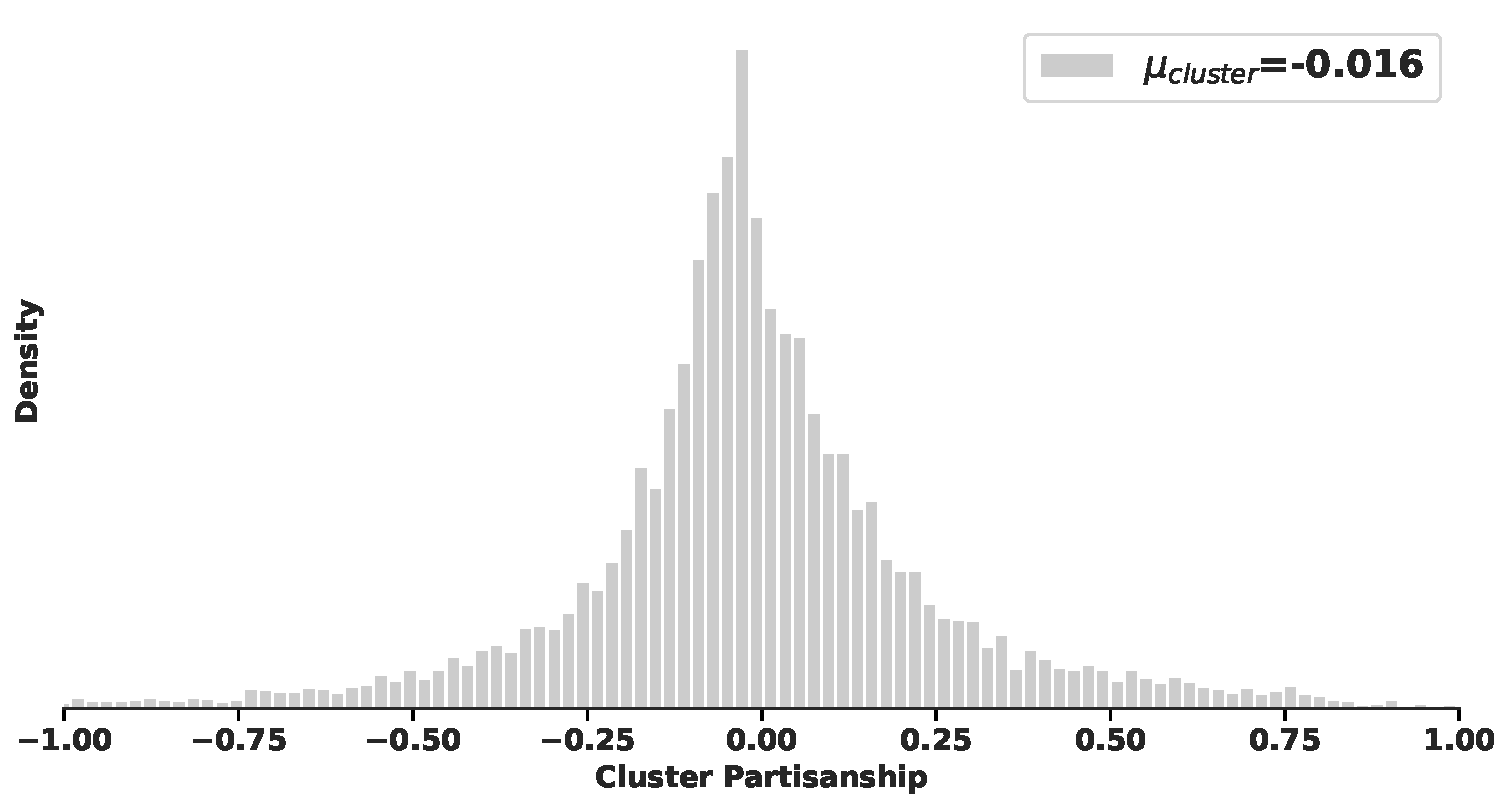
\includegraphics[width=1\columnwidth]{figures/cluster_partisanship_dist3.pdf} 
\caption{}
\label{fig:cluster-dists-part}
\end{subfigure}
\caption{The distribution of toxicity and partisanship within our set of clusters.}
\end{figure}

\vspace{2pt}\noindent
\noindent
\textbf{Estimating the Toxicity of Topics.}
To estimate the toxicity of particular topics, we determine the average toxicity score of all tweets present within that given cluster. While we largely rely on our average toxicity scores, in addition to this metric, we further determine the \emph{percentage} of toxic tweets within our \emph{entire} English-language dataset that conforms to that particular topic.  Namely, after identifying each toxic cluster center, for each of these toxic cluster centers, we further identify the set of non-toxic tweets that also conform to the topic. We then calculate the percentage of toxic tweets (\textit{i.e.}, toxicity > 0.5) per topic. 

To assign non-toxic tweets to our set of toxic tweet centers, we utilize the approach laid out in prior work~\cite{hanley2022happenstance,hanley2023partial} and subsequently assign each non-toxic tweet to the cluster center with the highest semantic similarity to the tweet. As recommended by Hanley {et~al.}~\cite{hhanleyspecious2024}, given our fine-tuned version of MPNet, we again utilize a cluster threshold of 0.60 for assigning a given non-toxic tweet to a given cluster. We plot the distribution of estimated topic toxicity in Figure~\ref{fig:cluster-dists-toxic}. We utilize this approach, rather than clustering all 89.6 million English tweets given the size of our dataset, and because, for this work, we largely are only concerned with topics that have some level of toxicity. 

\vspace{2pt}\noindent
\noindent
\textbf{Estimating the Partisanship of Topics.}
To further examine the role of partisanship within interactions within particular topic clusters, we further determine the overall political orientation of each cluster. To do so, after assigning all remaining non-toxic tweets to our clusters as specified above, we subsequently determine which set of users participated/tweeted about that topic. Calculating the average and standard deviation of the political orientations of all the Twitter users (utilizing our previous calculations of user partisanship [Section~\ref{sec:background-ca}]) that tweeted about that topic, we thus estimate each topic's political-ideological composition. We plot the distribution of the partisanship of our set of clusters in Figure~\ref{fig:cluster-dists-part}. 


\subsection{The Most Toxic Topics of 2022\label{sec:most-toxic}}

\begin{table*}
\centering
\scriptsize
\selectfont
\setlength{\tabcolsep}{4pt}
\begin{tabularx}{\textwidth}{lXrrrXrrr}
\toprule
 &   &  &   \# Toxic & Avg.& Example & Avg.  & Avg. Partisan  & Partisan \\
 Topic& {Keywords}&\# Tweets &Tweets  & Toxicity &  Tweet  & Partisan. & of Toxic Users& Std. \\
\midrule
 1 & biden, joe, administration, president, senile  &246,868 & 39,102 (15.84\%) & 0.1824& Joe Biden And everything is screwed up. You suk & 0.642 &0.379 &1.084\\ 

 2 & ukraine, russia, kyiv, putin, independent &763,153 & 36,425 (4.77\%) &0.070 &  So l guess you what Ukraine to stop fighting back and let the Russians kill them. Ukraine Will Resist Fuck Putin& -0.091 &0.031 & 0.899\\ %\hline

3 & lie, pathological, truth, habitual, liar  &100,825 & 26,894 (26.67\% ) &0.298 & These leftist serial liars always project onto others the crimes they are perpetrating. & -0.055 & 0.081 & 1.0300  \\

 4 & party, democrat, republican, dnc, destroying &111,763 & 22,705 (20.32\%) &0.232 & That slate is FAR better than the gaggle of corrupt Marxists the racist lunatic democrat party pushed forward. Nobody is gonna give you a nod for badmouthing the better team.
  &0.215&  0.171 & 1.162\\

  
 5& ballot, election, stolen, voting, rigged& 295,356 &  22,399 (7.58\%) &0.093 & You already know that the Maricopa County Election will say "Fuck Your Ballots" and ram it through the certifications.& 0.199 & 0.121 & 1.131 \\

  6 & fox, news, murdoch, carlson, tucker & 179,224 & 20,958 (11.69\%) &0.138 &Fox News Give it a rest already. For is even worse than national enquirer for false made up trash. & -0.027 & 0.089 & 1.116 \\

  7 & filipkowski, ron, flynn, bannon, nut & 107,255& 19,018 (17.73\%)&0.187 & @REDACTED Man are Fox ppl nuts or what &-0.686 & -0.535 & 0.784  \\

  8 & tweet, follow, deleted, algorithm, account & 190,665 & 18,822 (9.87\%)  &0.102& Ok is anybody else's twitter completely fucked up and glitchy?
 & 0.044 &  0.038 & 0.982\\

  9 & stupidity, smart, intelligent, educated, dumb & 23,232 & 18,533 (79.77\%)&0.688 &@I mean how stupid are these people or what?
What happened to like history classes?
Gees what a bunch of loser white people.&  0.141 &  0.131 & 0.938 \\

  10 & abortion, birth, pro-life, pregnancy, fetus &309,723 & 18,456 (5.96\%)&0.087& This moron thinks the Supreme Court literally edited the Bill of Rights to remove the right to an abortion. Dumb as fucking rocks these people.
 &  0.114 &.112 & 1.265 \\

\bottomrule
\end{tabularx}
\caption{Top toxic topics---by the number of toxic tweets---in our dataset.\label{table:toxic-topics}} 
\end{table*}
We start this section by providing an overview of the topics with the most toxic tweets in 2022 (Table~\ref{table:toxic-topics}). We further give an overview of the most partisan topics in Appendix~\ref{sec:partisan-toxic} and the most toxic topics in Appendix~\ref{sec:most-toxic-by-percentage} (most of these topics are merely users calling each other different epithets). As seen in Table~\ref{table:toxic-topics}, many of the most common toxic tweets concerned the most politically divisive issues of 2022~\cite{Montanaro2022}, namely, Joe Biden's administration (Topic 1;~246,968K tweets), Russia's invasion of Ukraine (Topic 2;~763K tweets), and the abortion rights in the United States in the wake of the Dobss v. Jackson decision which overturned US federal abortion rights~\cite{StaffAborrtion2022}.

Examining the average partisanship of the user who tweeted about each of the top toxic topics, we find distinct political differences. Markedly, we observe, that those who tweeted in a toxic manner about the Ukraine War tended to have a slight rightward tilt (+0.122 rightward tilt). Examining these tweets, we find right-leaning users when tweeting about the war, excoriated or derided the Ukrainian government or military, which was picked up as toxic by our contrastive-DeBERTa model. 
For example, one ``toxic'' tweet by a rightward user stated: 
\begin{displayquote}
\small
\textit{
No more arms for a Ukraine refusing to negotiate! Ukraine doesn't need more arms, Ukraine needs more intelligence! And Zelensky is a dictatorial asshole!}

\end{displayquote}
In contrast, considering all users who tweeted about the war, we find that they tended to lean leftward (-0.091 leftward tilt) with one left-leaning user tweeting:
\begin{displayquote}
\small
\textit{
Stand With Ukraine!}
\end{displayquote}
Looking at the users who tweeted about Joe Biden's presidency (Topic~1),  we again see a rightward bias (+0.642) among users who tweeted about him or his administration generally and with users who tweeted about him in a toxic manner (+0.379). For example, one user tweeted
\begin{displayquote}
\small
\textit{
Save the poor water bottle from that pedophile Joe Biden before he becomes a victim}
\end{displayquote} We thus observe that those talking about the administration (both in a toxic and non-toxic manner) were largely right-leaning (as largely expected given that the Biden administration is Democratic). Finally, examining the set of users who tweeted about abortion in 2022 (Topic~10), we again find a rightward lean among users who tweeted about this issue. For example, one right-wing user wrote:
\begin{displayquote}
\small
\textit{Why are actors so ignorant about policies? States can still do abortions. Go ahead and murder more babies.}
\end{displayquote}



Besides these politically salient issues, we observe several topics where politically charged users simply derided each other (Topic~4), called each other idiotic (Topic~9), or called the other political side liars (Topic~3). We further see in Topic~5 heavy emphasis on the US presidential election being stolen in Arizona. As documented by Prochaska et~al., a misinformation story called Sharpiegate where ``Sharpies invalidated ballots in Maricopa County, Arizona'' was widely spread on Twitter and we see evidence of it in our dataset with several political users heatedly and toxically calling the Arizona election rigged~\cite{prochaska2023mobilizing}.





\subsection{Topic Dependent Changes in Partisanship and Toxicity \label{sec:changes}} Having explored some of the most prominent toxic topics during our period of study, we now explore how the toxicity of different Twitter topics change as users of different political orientations enter and leave. We find that regardless of whether a topic moderates (\textit{i.e.}, political orientation moves closer to 0) or becomes more extreme (\textit{i.e.}, political orientation becomes more left-leaning or more right-leaning), on average, this movement has little bearing on toxicity. Indeed correlating the change in the political orientation of a given topic between January and December with the percentage change in the toxicity of that conversation, we calculate a Pearson correlation of $\rho=-0.0168$, indicating little to no relationship. Similarly, we find that the variance of political participation in particular topics over time is also only slightly correlated with the toxicity of a given topic $\rho=-0.098$. This indicates that unlike for users, a different dynamic may be influencing the toxicity of particular topics across time. 

Across our dataset, we find that regardless of whether the topic moderates or moves to the extremes, in both cases, toxicity generally increases (55.8\% of the time for topics that moderated in partisanship and 71.4\% of the time for topics that moved to the political extreme). Furthermore, we find that between January 2022 and December 2022, in 34.8\% of topics, as topics became more right-leaning, they also became more toxic; in 27.1\% cases, they became less toxic as they became more right-leaning. Conversely, in 21.2\% of our topics, they became more toxic as they became more left-leaning, and in  17.0\% of topics they became less toxic as they became more left-leaning. However, examining each cluster, we \emph{do} find that on a cluster-by-cluster basis as the political composition of users involved in that topic changes there are corresponding changes in toxicity.

\begin{figure}
\begin{subfigure}[l]{0.32\textwidth}
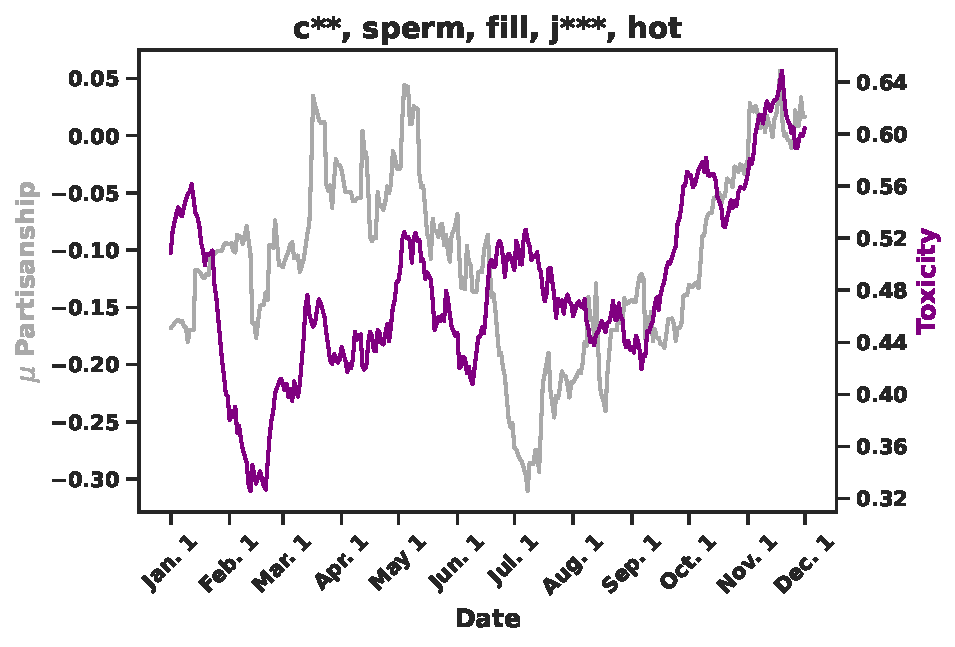
\includegraphics[width=1\columnwidth]{figures/c__-toxic-swing-final-20240425.pdf} 
\caption{}
\label{fig:cum}
\end{subfigure}
\begin{subfigure}[l]{0.32\textwidth}
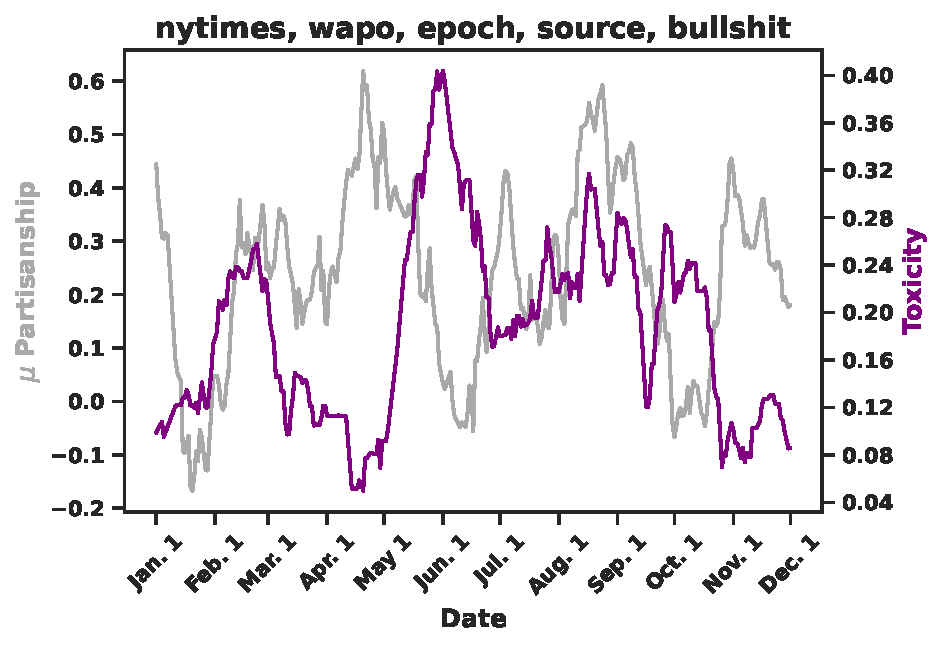
\includegraphics[width=1\columnwidth]{figures/nytimes-toxic-swing-final-20240425.pdf} 
\caption{}
\label{fig:nytimes}

\end{subfigure}
\begin{subfigure}[l]{0.32\textwidth}
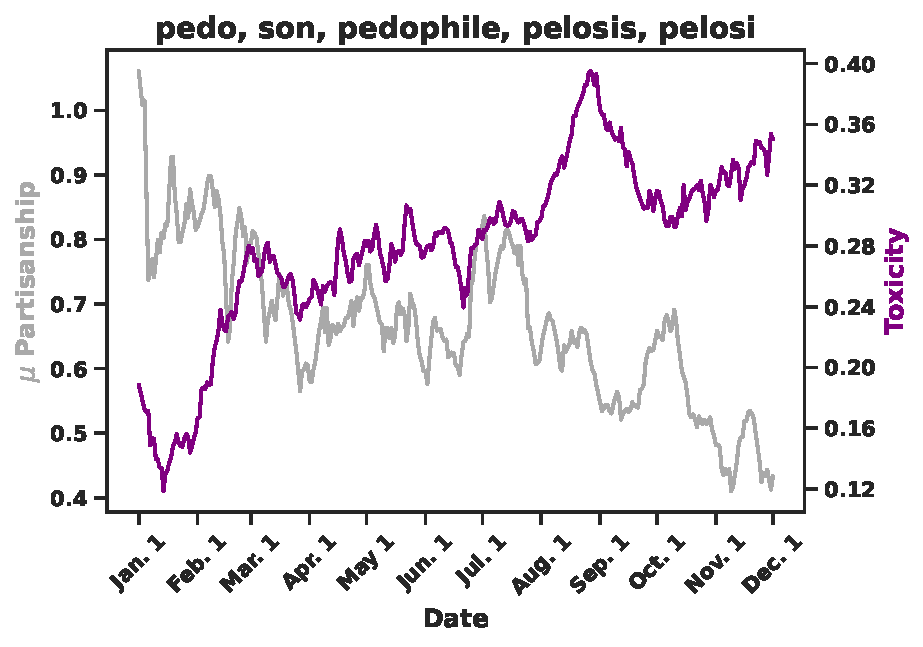
\includegraphics[width=1\columnwidth]{figures/pedo-toxic-swing-final-20240425.pdf} 
\caption{}
\label{fig:pedo}
\end{subfigure}
\begin{subfigure}[l]{0.32\textwidth}
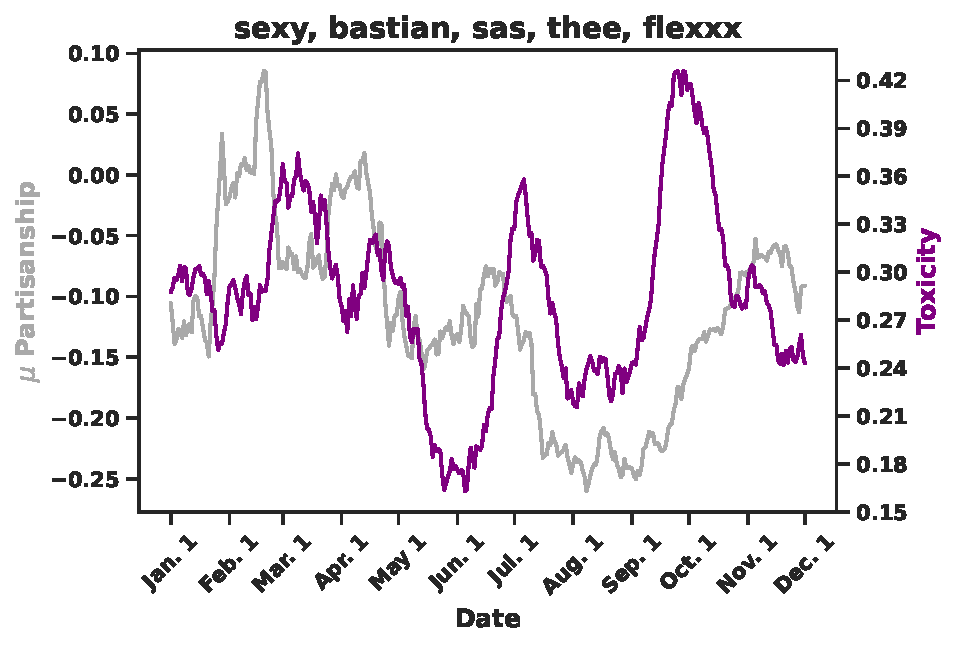
\includegraphics[width=1\columnwidth]{figures/sexy-toxic-swing-final-20240425.pdf} 
\caption{}
\label{fig:sexy}
\end{subfigure}
\begin{subfigure}[l]{0.32\textwidth}
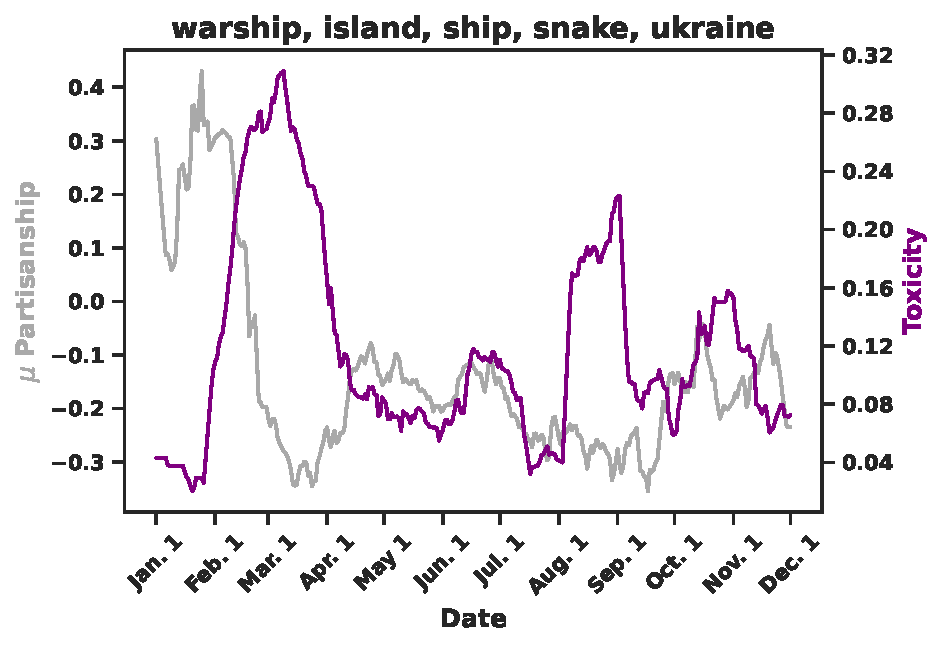
\includegraphics[width=1\columnwidth]{figures/warship-toxic-swing-final-20240425.pdf} 
\caption{}
\label{fig:warship}
\end{subfigure}
\begin{minipage}[l]{1\textwidth}
\caption{Topics with the largest increase in toxicity in 2022. \label{fig:toxicity-swing}}
\end{minipage}
\vspace{-15pt}
\end{figure}



\begin{figure}
\begin{subfigure}[l]{0.32\textwidth}
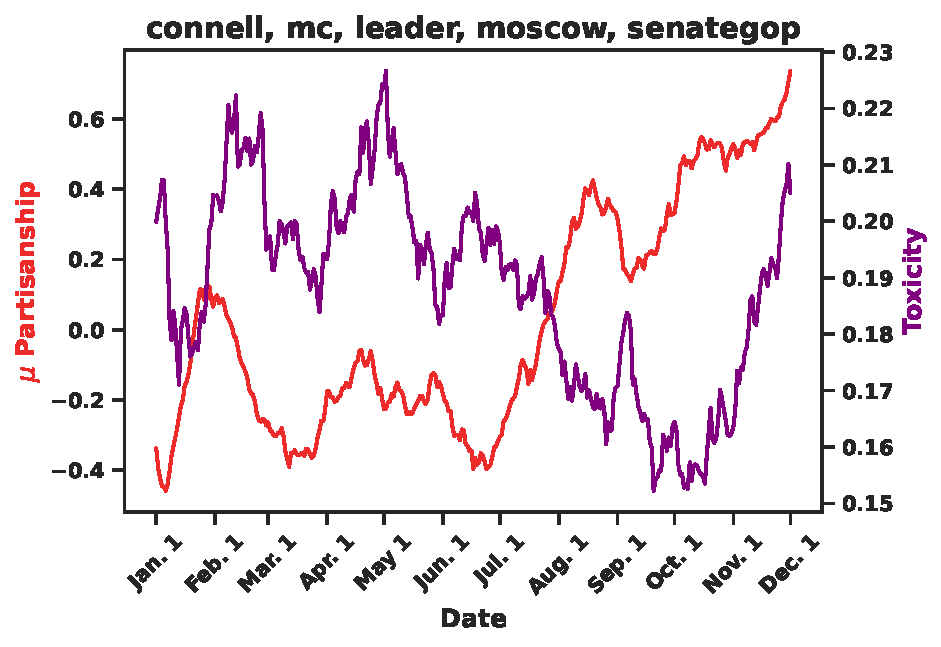
\includegraphics[width=1\columnwidth]{figures/connell-conservative-final-20240425.pdf} 
\caption{}
\label{fig:moscow}
\end{subfigure}
\begin{subfigure}[l]{0.32\textwidth}
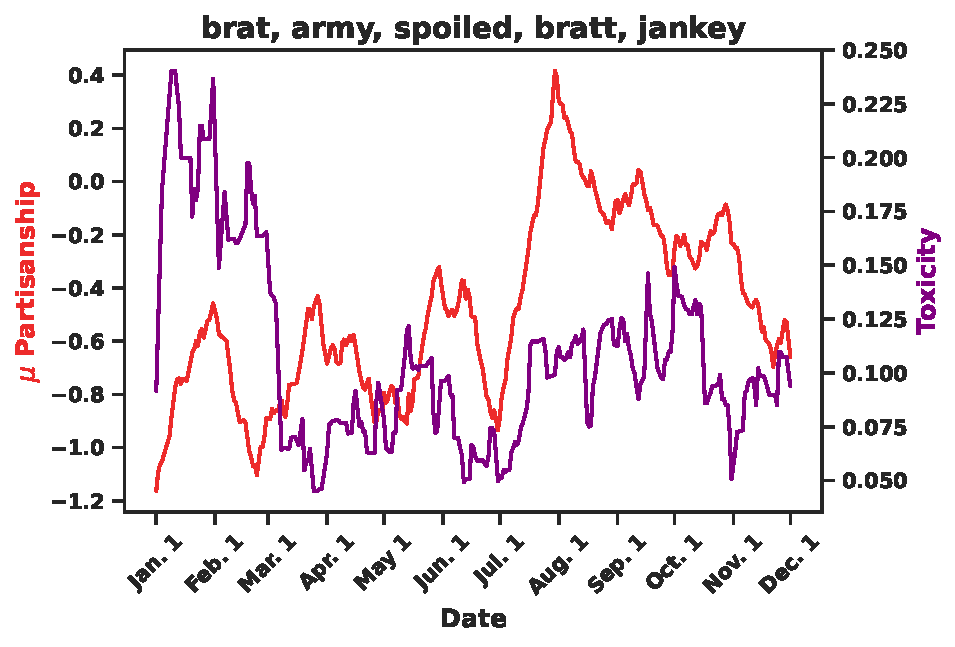
\includegraphics[width=1\columnwidth]{figures/brat-conservative-final-20240425.pdf} 
\caption{}
\label{fig:brat}
\end{subfigure}
\begin{subfigure}[l]{0.32\textwidth}
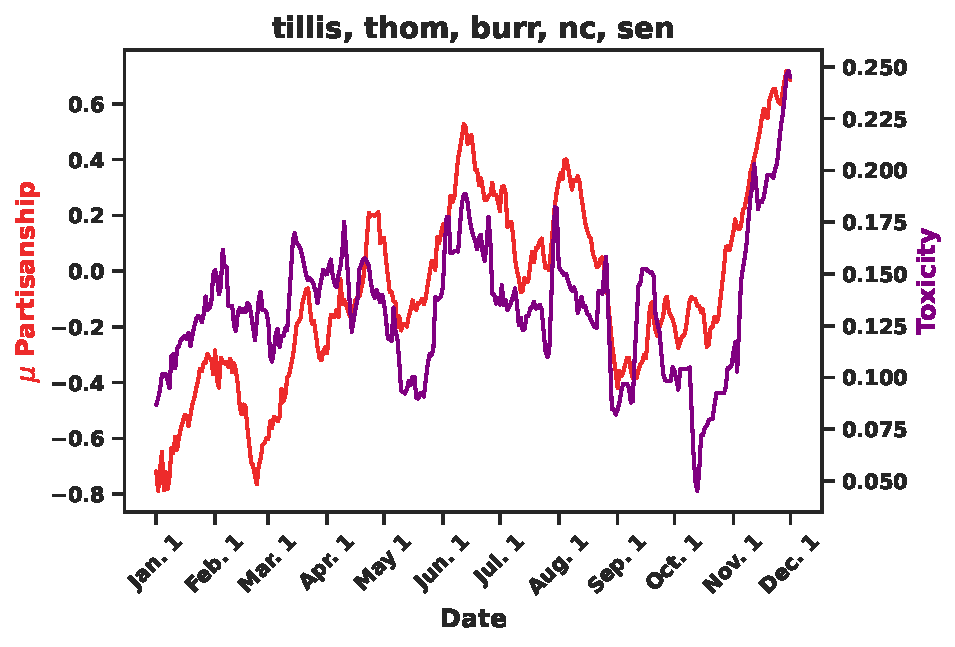
\includegraphics[width=1\columnwidth]{figures/tillis-conservative-final-20240425.pdf} 
\caption{}
\label{fig:tillis}
\end{subfigure}
\begin{subfigure}[l]{0.32\textwidth}
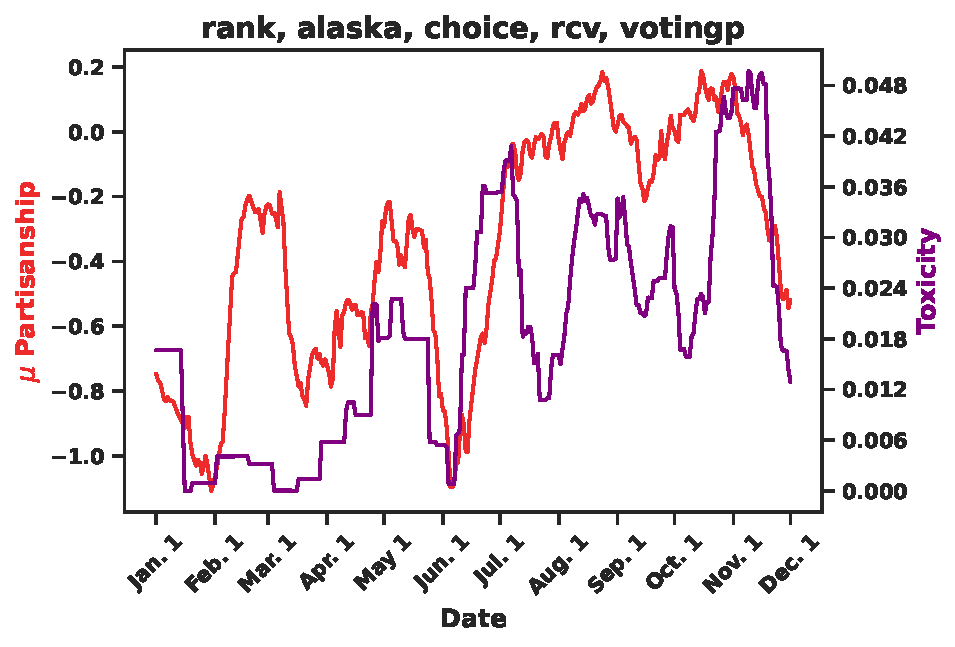
\includegraphics[width=1\columnwidth]{figures/rank-conservative-final-20240425.pdf} 
\caption{}
\label{fig:rank}
\end{subfigure}
\begin{subfigure}[l]{0.32\textwidth}
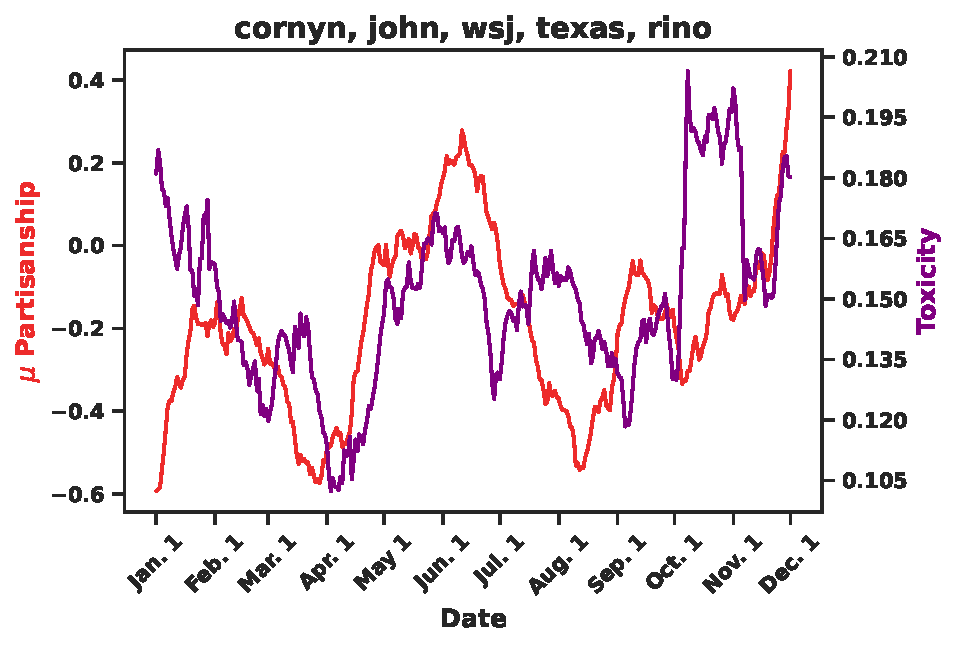
\includegraphics[width=1\columnwidth]{figures/cornyn-conservative-final-20240425.pdf} 
\caption{}
\label{fig:cornyn}
\end{subfigure}
\begin{minipage}[l]{1\textwidth}
\caption{Topics with the largest swing to right-leaning partisanship throughout 2022. \label{fig:conservative-swing}}
\end{minipage}
\end{figure}


\vspace{2pt}
\noindent
\textbf{Toxic Swings.} To further qualitatively understand the nature of how toxicity and political orientation change over time, we plot the toxicity and partisanship for the topics with the largest increases in toxicity between January 2022 and December 2022. We observe that while for four topics considered, (Figures~\ref{fig:cum},~\ref{fig:nytimes},~\ref{fig:sexy}, and~\ref{fig:warship}) as the topic became more right-leaning, toxicity similarly increased, for one of the topics (Figure~\ref{fig:pedo}), we observe the opposite. Examining, each we observe, noticeable trends where, depending on the political nature of the topic,  a corresponding swing in the political composition of the users in the left or the right direction, is correlated with an increase in toxicity. For instance, in the tweets surrounding the New York Times and the Washington Post's accuracy,  we observe that as users discussing the topic became more right-leaning, the more toxic the tweets. We similarly find for the topic surrounding the destruction of Russian warship on Snake Island by Ukrainians, the more right-wing the users, the more toxic. For example, one user wrote:
\begin{displayquote}
\small
\textit{
    Surprising Russian Navy Losses Against Ukraine Century After Tsushima 
Ukraine is really FUCKING Russian Navy Ship's up during the Russian Invasion into Ukraine}
\end{displayquote}

\noindent
In contrast, for Topic 3 (Figure~\ref{fig:pedo}), we observe that as users became more left-leaning the overall toxicity of the topic decreased. We observe that this is largely due to left-leaning users adopting retorts to right-leaning users calling the Democratic former Speaker of the House Nancy Pelosi a pedophile. For example, we observe one user stating:

\begin{displayquote}
\small
\textit{
Let's not forget that the last republican speaker of Michigan house was a Pedophile who raped a 15 year old sister in law.}
\end{displayquote}

\noindent
We thus observe among these top topics that depending on the political nature of the given topic and how users are interacting and replying to other users about the topic, a corresponding swing in the political composition of the users in the opposite direction, may or may be correlated with an increase in toxicity. 



\noindent
\vspace{2pt}
\textbf{Left-Leaning and Right-Leaning Swings.} Plotting the set of topics with the largest swings in average political orientation, to both the right and left-leaning end, between January 2022 and December 2022 (Figures~\ref{fig:conservative-swing} and~\ref{fig:liberal-swing}), we again observe that changes in toxicity as a result of these changes are largely dependent on the topic. For example, as the conversation surrounding Tom Tills (the senior Republican Senator for North Carolina) became more right-leaning, the toxicity of that topic increased dramatically (Figure~\ref{fig:tillis}). Despite Senator Tillis being a Republican, we observe that this is largely due to right-leaning users largely labeling Senator Tillis a RINO (Republican in name only) with one user posting:

\begin{displayquote}
\small
\textit{You've always been a RINO
NC must be ashamed of you}
\end{displayquote}
\noindent We find a similar behavior for Senator John Cornyn of Texas, again with a user writing:

\begin{displayquote}
\small
\textit{John Cornyn This Bill is trash. RINOs need to go.
Cornyn votes with the Democrats almost as often as his own party.
Texas should be ashamed}
\end{displayquote} We similarly find that as right-leaning users joined the conversation about US Senate Republican Minority Leader Mitch McConnell being beholden to the Russian government~\cite{Hulse2018} toxicity increased. We note that the attacks against Senators Mitch McConnell, John Cornyn, and Tom Tillis were \emph{all} largely for not being conservative enough. Finally, for Democratic Manhattan District Attorney Alvin Bragg, we also observe that when more right-leaning users joined the conversation surrounding him, toxicity increased. However, unlike for the Republican Senators, more intuitively, this was largely due to his investigation of former Republican President Donald Trump. 

In contrast, for Republican Ohio Governor Mike DeWine, we observe that as more left-leaning users joined the conversation surrounding him the topic became more toxic, with one user writing
\begin{displayquote}
\small
\textit{
Gov Mike DeWine Thank you, Gov Mike DeWine, for making it easier for Ohioans to be killed by gun violence. Fuck you.}
\end{displayquote}
Similarly, for Republican Florida Congressman Matt Gaetz, we also observe that as more liberal users joined the discussions surrounding him the topic became more toxic. We find that this was largely sparked by a tweet from Matt Gaetz stating:

\begin{displayquote}
\small
\textit{Over-educated, under-loved millennials who sadly return from protests to a lonely microwave dinner with their cats, and no bumble matches.}
\end{displayquote}
\noindent to which one user replied 
\begin{displayquote}
\small
\textit{Only stupid, insecure men worry about women being over-educated. Which one are you, matt gaetz?}
\end{displayquote}

\noindent
We thus observe that the context of each of these topics, in particular, is decisive for determining how different swings in political polarization will affect the overall toxicity of the topic. As within individual users (See Section~\ref{sec:toxic_middle}), partisanship itself does not necessarily predict a higher degree of toxicity within conversations but is largely topic-dependent. Even the target/topic being a right-leaning or left-leaning entity/individual not decisively giving whether a left or right-leaning shift in users will correspond to an increase in toxicity. 

\begin{figure}
\begin{subfigure}[l]{0.32\textwidth}
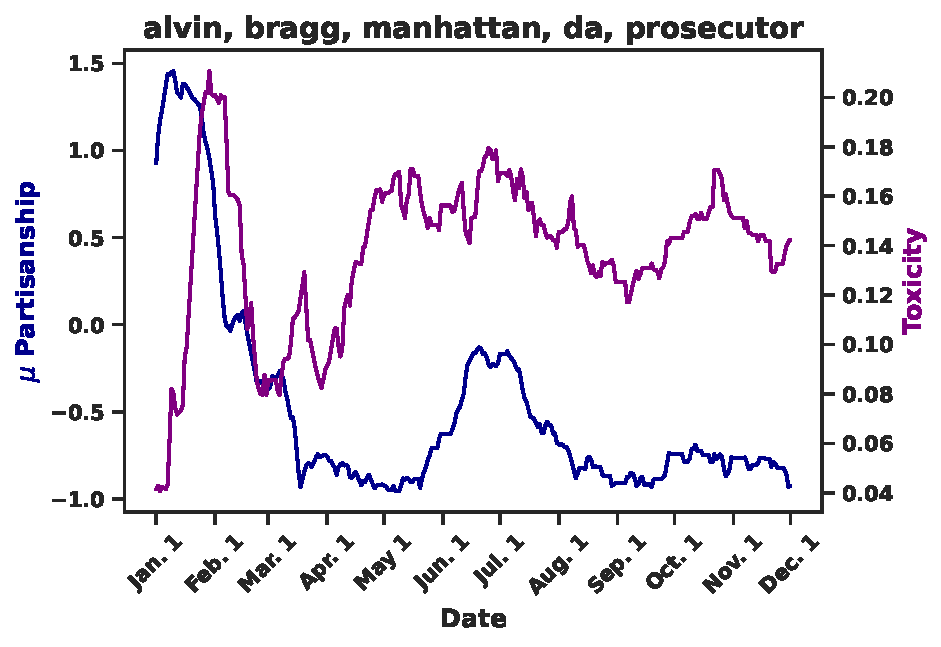
\includegraphics[width=1\columnwidth]{figures/alvin-lib-final-20240425.pdf} 
\caption{}
\label{fig:alvin}
\end{subfigure}
\begin{subfigure}[l]{0.32\textwidth}
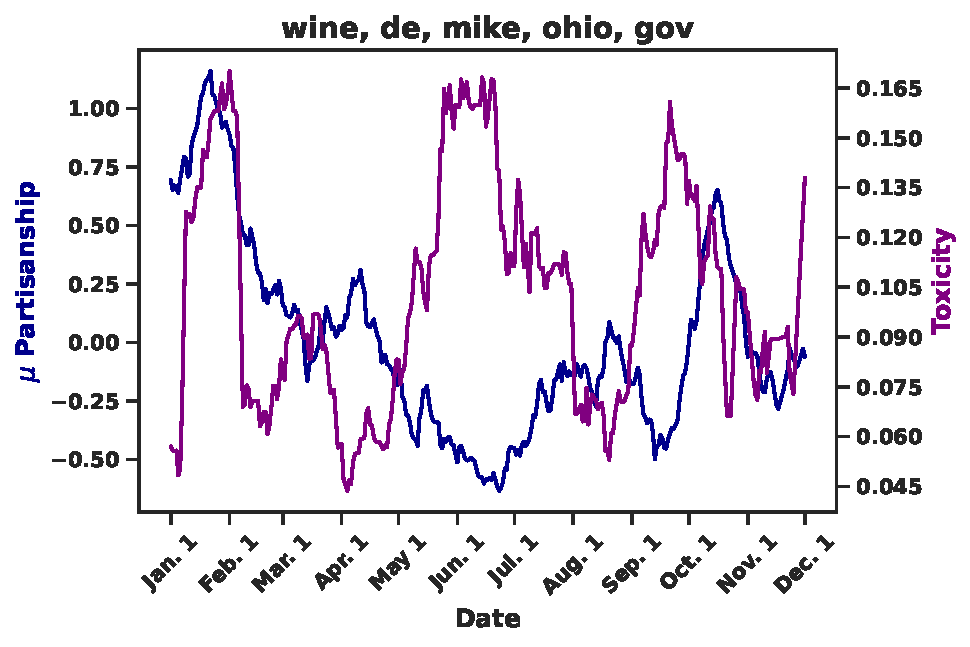
\includegraphics[width=1\columnwidth]{figures/wine-lib-final-20240425.pdf} 
\caption{}
\label{fig:wind}
\end{subfigure}
\begin{subfigure}[l]{0.32\textwidth}
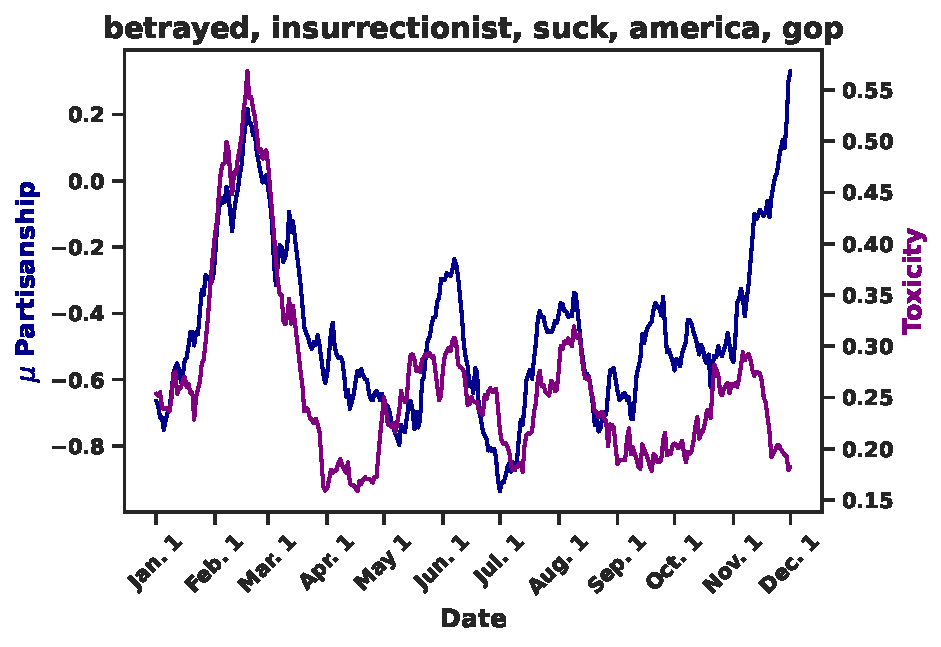
\includegraphics[width=1\columnwidth]{figures/betrayed-lib-final-20240425.pdf} 
\caption{}
\label{fig:betrayed}

\end{subfigure}
\begin{subfigure}[l]{0.32\textwidth}
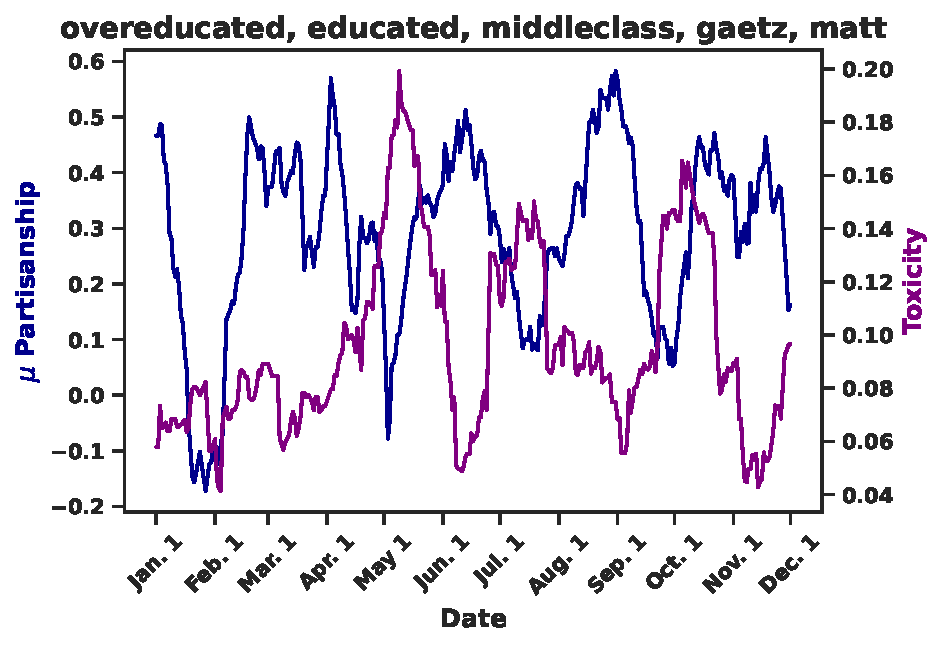
\includegraphics[width=1\columnwidth]{figures/overeducated-lib-final-20240425.pdf}
\caption{}
\label{fig:overeducated}
\end{subfigure}
\begin{subfigure}[l]{0.32\textwidth}
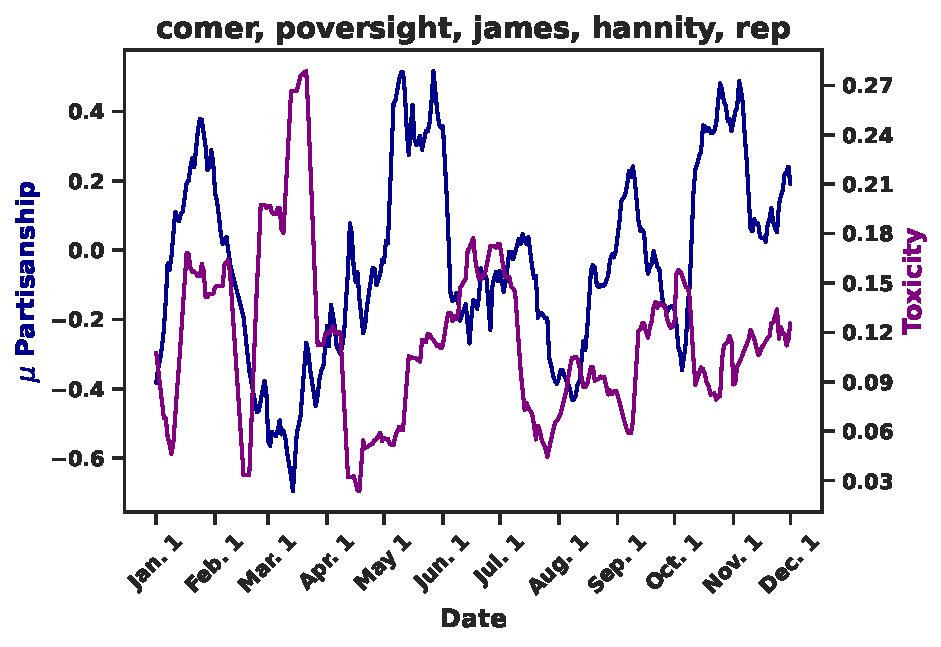
\includegraphics[width=1\columnwidth]{figures/comer-lib-final-20240425.pdf} 
\caption{}
\label{fig:comer}
\end{subfigure}


\begin{minipage}[l]{1\textwidth}
\caption{Topics with the largest swing to left-leaning partisanship throughout 2022. \label{fig:liberal-swing}}
\end{minipage}

\end{figure}

\subsection{Topic User Composition and the Toxicity of Topics\label{sec:topic-level-gam}} Having qualitatively described the composition and changing dynamics of some of our set of topic clusters, we now determine how the several user-level features of individual topic clusters predict the toxicity within the topic to better understand what may be influencing the toxicity of individual topics.

We note, and as seen throughout this section, topics on Twitter vary widely with individual topics often varying widely in political composition over time. Across all topics considered in our dataset, on average between January 2022 and December 2022, the political composition of the users tweeting about each topic changed by 0.159 standard deviations (based on the latent space that we previously determined [Section~\ref{sec:background-ca}]). In 61.9\% of cases, topics became more right-leaning, and in 38.1\%  topics became more left-leaning; similarly, within this same period, 56.0\% became more toxic while 44.0\% became less toxic. As a result, to quantify the effect that the composition of users has on the toxicity of a given topic at a single point in time, for each topic and each month combination, we gather the user compositions and the cluster characteristic data. We thus, in this section seek to determine the factors that determine the average toxicity score of a topic within a single month time-span. 

As before, to determine the role of various topic-level features in the overall toxicity of that cluster, we fit a GAM on the average toxicity score each month within each of our clusters against: \begin{enumerate}
    \item \emph{The number of users who tweeted about that topic.}
    \item \emph{The average user toxicity in the cluster.}
    \item \emph{The percentage of users involved in that topic that is Twitter verified.}
    \item \emph{The average of the partisanship in that cluster.}
    \item \emph{the standard deviation of political ideologies of users within that topic cluster.}
    \item \emph{The average age of the users in clusters.}
\end{enumerate}

Again, as in Section~\ref{sec:toxic_middle} when fitting our model, we perform variable selection based forward selection based on the Akaike Information Criterion~\cite{akaike2011akaike} Furthermore, again, to ensure that our model generalizes, we reserve out 10\% of our data as validation, and in our results report our model's $R^2$ value on this validation set. After fitting this regression, we further determine the estimated importance of each variable to our final model by permuting the features and seeing the estimated impact on the $R^2$ score of the validation set of our data. We do not consider other user account characteristics due to their multicollinearity with user toxicity (as seen in Section~\ref{sec:toxic_middle}, many user characteristics are correlated with their individual toxicity). Finally, we again reproduce our results with the Perspective Toxicity API in Appendix~\ref{sec:cluster-perspective-tox} obtaining similar results.


\begin{figure}
\begin{minipage}[l]{1.0\textwidth}
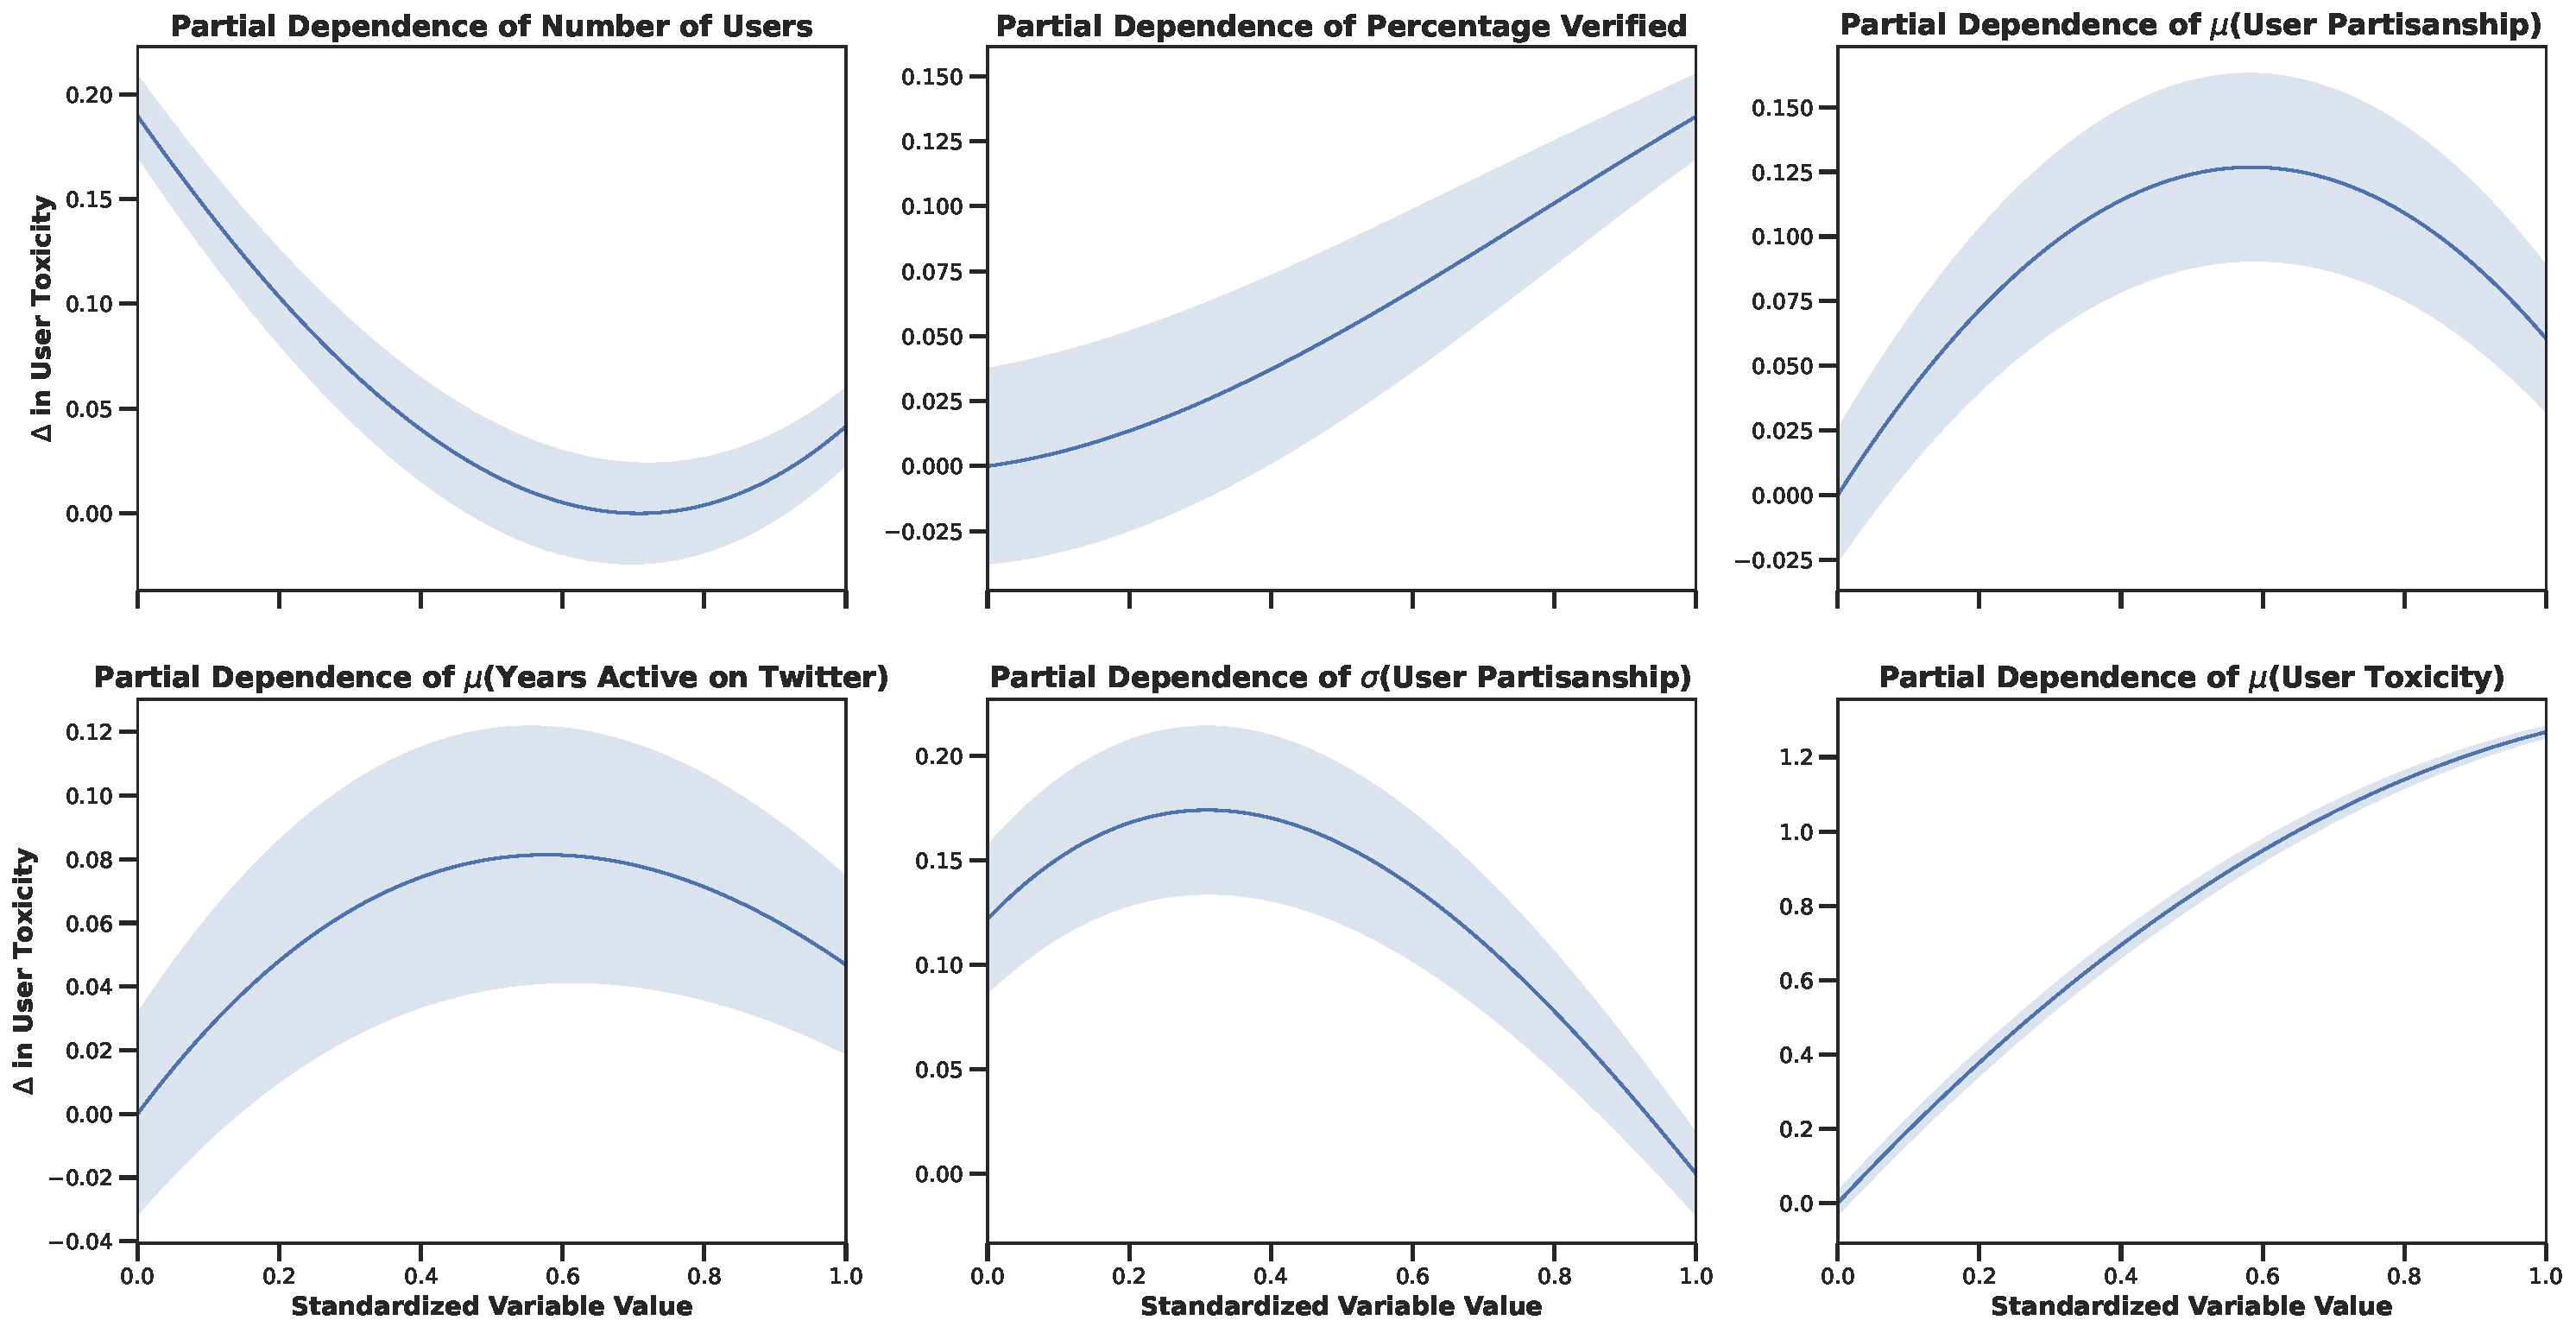
\includegraphics[width=1\columnwidth]{figures/partial_dependence_important_variables-clusterlevel-1.pdf} 
\end{minipage}
\begin{minipage}[l]{1\textwidth}
\caption{Partial dependencies with 95\% Normal confidence intervals between our fitted standardized dependent variables and cluster toxicity.}
\label{fig:partial-dependcies-clusterlevel}
\end{minipage}

\end{figure}

\begin{table}
    \small
    \centering
    \begin{tabularx}{0.85\columnwidth}{l|rrr}
     Train $R^2$: 0.397, Validation $R^2$:  0.389  \\
    \toprule
      Dependent Variable  & Pearson Corr. $\rho$ & Kendall's $\tau$ & Permut Import. \\    \midrule
  Number of Users &-0.292 & -0.139  & 0.445  \\
 $\mu$(Years Active on Twitter) &-0.191 & -0.186 & 0.018\\
  Percentage Verified &0.234 & 0.250 & 0.007  \\
$\sigma$(User partisanship) & 0.098 & 0.003 & 0.021 \\
  $\mu$|User partisanship) & 0.028 &  0.005 & 0.007 \\
  $\mu$(User Toxicity) &  0.589 & 0.486 & 0.502 \\
    \bottomrule

    \end{tabularx}
  \caption{Pearson correlation $\rho$ and Kendall's $\tau$ of dependent variables and clusters' toxicities. } 
   \vspace{-15pt}
   \label{table:regression-clusterlevel}
\end{table}




As seen in Table~\ref{table:regression-clusterlevel}, and Figure~\ref{fig:partial-dependcies-clusterlevel}, unsurprisingly, the most important factor in determining the toxicity of a given topic is the toxicity of the users contributing tweets to the cluster. This one variable has a permutation importance of 0.50 and a correlation of 0.58 with the toxicity of a given cluster. Simply put, unsurprisingly, topics whose corresponding users have higher average toxicity are more likely to have toxic content. As in Section~\ref{sec:toxic_middle}, we again observe being further along the political spectrum does not necessarily indicate increased toxicity and that a conversation being dominated by right-leaning or left-leaning users has little bearing on its toxicity. 

We find, as seen in Figure~\ref{fig:partial-dependcies-clusterlevel}, that the number of users involved in a given topic appears to have a moderating and mitigating effect on the toxicity of that topic ($\rho=0.292$). This also appears as one of the most important features for determining the average toxicity with a permutation score of 0.445. However, conversely having more verified individuals participating in that topic \emph{does} increase toxicity. We thus find (from Section~\ref{sec:toxic_middle}) that while verified users are less likely to tweet toxic content, their presence and their tweeting about particular topics correlate with increased toxicity in that topic. We further find that despite the average age of accounts participating in a topic having a negative Pearson correlation in our fitted model if the average age of the accounts participating in a conversation is very young or much older, there is a decreased toxicity compared to topics that engage accounts of all ages.

Examining political ideological contributions in Figure~\ref{fig:partial-dependcies-clusterlevel}  to the toxicity of individual topics we find that topics dominated by all left-leaning or all right-leaning users are largely the least topics compared to topics in the middle of the ideological spectrum. Finally examining the partial dependence of the diversity of viewpoints that participate in a given topic at a given point in time, we find that while initially the greater the political diversity of the topic cluster, the more toxic it becomes, as the topic invites more and more users of different beliefs that the topic cluster decreases in toxicity. While further research is needed, this result reinforces the work of Mamkos et~al. that find that for particular typically non-political topics that engage users from all over the political spectrum, these topics tend to be less toxic than others~\cite{mamakos2023social}.

 \begin{figure}
\begin{minipage}[l]{0.6\textwidth}
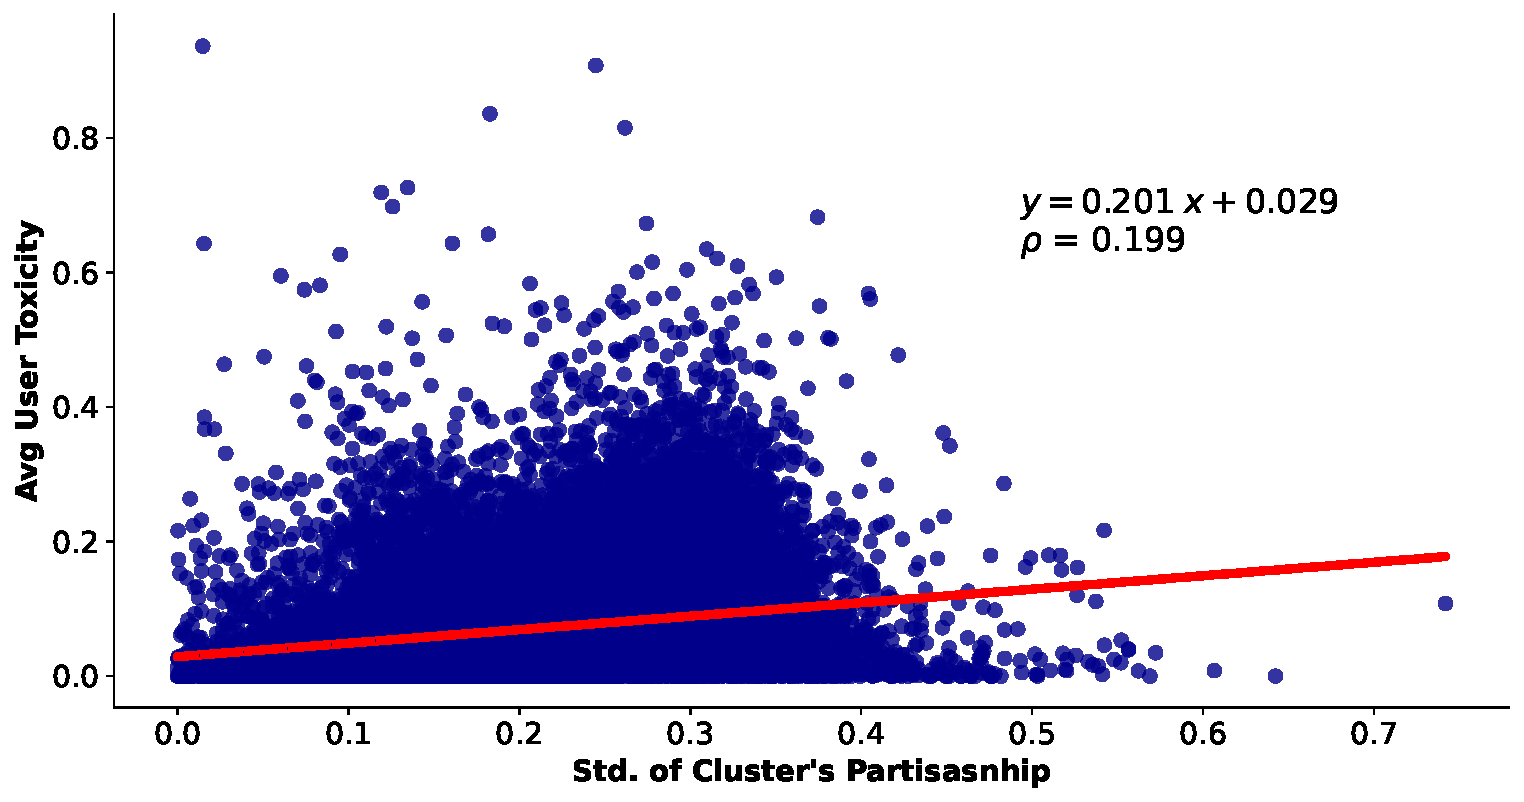
\includegraphics[width=1\columnwidth]{figures/cluster_user_ideology_vs_user_toxicity-20240429.pdf} 
\end{minipage}
\begin{minipage}[l]{0.33\textwidth}
\caption{As previously also found in our analysis of user characteristics (Section~\ref{sec:calculated}), we find that as users engage in a wider window of topics of particular political ideologies, the more toxic their tweeted content\label{fig:toxicity-vs-var-user}}
\end{minipage}

\end{figure}


Lastly, looking in the reverse direction, we determine how users' toxicity changes when they are involved in many different types of politically aligned topics.  As also found by Mamkos et~al.~\cite{mamakos2023social}, we find, as seen in Figure~\ref{fig:toxicity-vs-var-user},  as users are involved in a higher variance of topics of different political orientations their average toxicity increases ($\rho=0.19$). We thus find from this analysis further confirmation, on a topic level, that increased user toxicity and the diversity of views present in a given conversation contribute to toxicity within particular topics. However, conversely, as topics invite a wider range of individuals into a discussion toxicity actually decreases. We now consider some of the implications of these results. 










%\section{RQ1: Reddit Misinformation Submissions vs Authentic News Submissions}\label{sec:rq1}
Having outlined our methodology, in this section we turn to understand the relative levels of toxicity and polarization orientations of users and subreddits that interact with misinformation and authentic news. 




%\subsection{Misinformation vs Mainstream Submissions}


\subsection{Experimental Setup}
As previously mentioned, on Reddit, users can submit news articles from different websites as a submission under which users can comment and discuss the article or issues prompted by the news article headline. To understand the relative presence of political incivility and toxic comments compelled by misinformation, we thus first compare levels of toxic comments posted under misinformation and authentic news URL submissions.

To do this, across all our collected subreddits we gather the sets the URL submissions that utilize our set of misinformation and authentic news websites. Altogether, within our Pushshift dataset, there were 38,264 different submissions utilizing our first set of 541 misinformation websites from 2,217 different subreddits and 226,930 submissions utilizing our first set of 565 authentic news websites from 18,383 unique subreddits. This difference in magnitude of submissions, we believe, is largely due to the greater popularity and widespread appeal of authentic mainstream news compared with alternative and more fringe websites. Indeed, utilizing the Amazon Alexa Top Million list from March 1, 2021~\cite{amazon-top-mil}, we find that 255 authentic news websites were in the top 100K websites, while only 101 misinformation websites were in the top 100K. To further bolster and confirm our results, we test our findings in this section utilizing our second set of misinformation and mainstream websites. Altogether, from this second set of URLs, we find an additional set of 9,558 misinformation and 560,673 authentic news submissions.

\subsection{Differences in Toxicity/Incivility between Misinformation and Authentic News Submissions}\label{sec:toxicity}

Looking at the toxicity comments from our first set of misinformation domains, we see that 14.9\% of the submission had at least one toxic comment and 1.35\% of all the comments were toxic. In contrast, for the first set of authentic submissions 13.6\% of the submissions had a toxic comment and only 0.85\% of the comments were toxic. We thus see a 60\% uptick in the rate at which toxic comments are posted on the misinformation submissions. Confirming this finding with our second set of 9,558 misinformation and 560,673 authentic news submissions, we again see a similar pattern of higher toxicity in the misinformation submission comments. 15.3\% of the misinformation submissions had toxic comments with 0.92\% of the comments being toxic. In contrast, 11.74\% of the mainstream submissions had toxic comments with 0.64\% of the comments being toxic. We thus see in this replicated experiment that Reddit misinformation conversations indeed have a higher incidence and occurrence of toxicity and incivility. Putting all these conversations together, we find that 1.17\% of comments under misinformation submissions are toxic/uncivil while 0.7\% of comments for authentic news websites are toxic/uncivil. we thus find an overall 63\% increase in the rate at which toxic comments are posted on misinformation submissions.

\begin{figure*}
\begin{subfigure}{.4\textwidth}
  \centering
  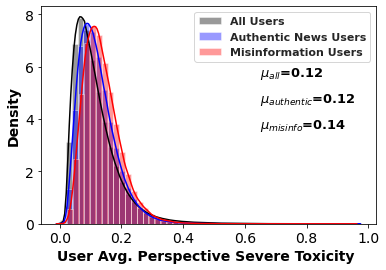
\includegraphics[width=1\linewidth]{figures/user_toxicity_above10.png}
  \caption{URL Set 1}
\label{fig:harmonic-sub1}
\end{subfigure}
\begin{subfigure}{.4\textwidth}
  \centering
  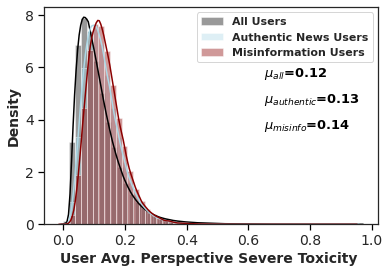
\includegraphics[width=1\linewidth]{figures/user_toxicity_above10_2.png}
    \caption{URL Set 2}
  \label{fig:pagerank-sub2}
\end{subfigure}

\caption{\textbf{Toxicity levels for users who comment under authentic News and misinformation URL Reddit submissions}---Users who interact with misinformation submissions are slightly more toxic/uncivil than users that interact with authentic news. Both groups are slightly more toxic/uncivil than Reddit users generally. }
\label{fig:users-misinformation-authentic-toxicity}
\end{figure*}
%\paragraph{User and Subreddit Toxicity in Misinformation and Mainstream Reddit Submissions }
%  We now seek to eke out some of the causes the higher amount of toxicity within the misinformation URL submissions on Reddit. 


Higher toxicity within misinformation submissions could be caused by (1) more toxic/uncivil users participating in these conversations or (2) higher toxicity norms in the subreddits where the misinformation was posted. As seen in Figure~\ref{fig:users-misinformation-authentic-toxicity}, we see that these users are slightly more toxic than their authentic news counterparts. For the first group of URL submissions, on average 1.54\% of the comments for the users associated with these submissions are toxic/uncivil compared with 1.22\% for the corresponding group of authentic news users. Similarly, on average 1.48\% of comments posted by the second group of misinformation users are toxic compared to 1.32\% for the authentic news commenters. However, for bot URL groups, as seen in Figure~\ref{fig:users-misinformation-authentic-toxicity}, the distributions of their Perspective API scores are fairly close. We note, that despite this proximity in toxicity of misinformation commenters between authentic news commenters, the higher user toxicity appears stable even among users from the same subreddits. Comparing the users who posted in subreddits where \emph{both} mainstream and misinformation URLs were posted, we still see that the users who posted on misinformation submissions had elevated rates of toxicity (1.21\% compared to 1.45\%). We thus see ``more toxic'' users are indeed commenting more on misinformation submissions compared to authentic news submissions. Finally, to further confirm our results, we perform U-Mann Whitney tests to ensure that there are indeed statistically significant differences between the rate of toxicity in misinformation and authentic news users; running these tests finding p-values $<10^{-12}$, we indeed conclude that both groups URL submission commenters that there are indeed higher rates of toxicity for the misinformation users.

However, despite the finding that more toxic users are indeed commenting more often on misinformation submissions, their higher rate of toxicity is not enough to explain the larger amount of toxic comments in misinformation submissions. After accounting for the higher rate of user toxicity across all the URL submissions, we still see 25.4\% more toxic comments than would be expected for the first set of URLs and 28.0\% for the second comparison set. Other factors, besides the specific users that comment on misinformation, are contributing to the higher rate of toxicity on misinformation submissions.



\begin{figure*}
\begin{subfigure}{.4\textwidth}
  \centering
  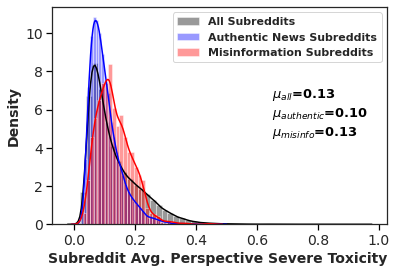
\includegraphics[width=1\linewidth]{figures/subreddit_toxicity_above10.png}
      \caption{URL Set 1}
\label{fig:harmonic-sub1}
\end{subfigure}%s
\begin{subfigure}{.4\textwidth}
  \centering
  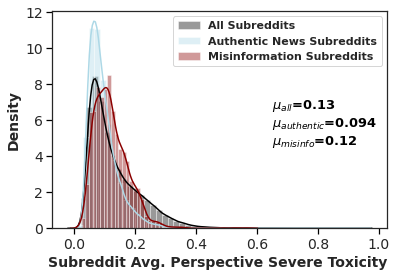
\includegraphics[width=1\linewidth]{figures/subreddit_toxicity_above10_2.png}
      \caption{URL Set 2}
  \label{fig:pagerank-sub2}
\end{subfigure}

\caption{\textbf{Toxicity Levels in Subreddits with Authentic News and Misinformation URL Submission}---Subreddits with misinformation submissions are overall more toxic/uncivil compared with authentic news subreddits and subreddits more generally.}
\label{fig:subreddit-misinformation-authentic-toxicity}
\end{figure*}

Looking at the role of subreddits in promoting toxicity in Figure~\ref{fig:subreddit-misinformation-authentic-toxicity}, we find that the toxicity norms of subreddits with misinformation submissions also contribute to higher levels of toxic comments. We see that on average for both sets of URLs that we consider, the set of subreddits with misinformation submissions have higher levels of toxicity compared to subreddits with authentic news submissions. Altogether, in our first set of misinformation URLs, for corresponding subreddits 1.40\% of comments posted there are toxic/uncivil. This is compared to a corresponding rate of 0.80\% for comments within subreddits with authentic news submissions. We see a similar difference from our second set of URLs (1.1\% vs 0.7\%). From these two datasets, we thus find that users in subreddits with misinformation submissions post toxic comments at a rate between 57\% (second set of URLs) and 75\% (first set of URLs) higher than in subreddits with authentic news submissions. We again perform U-Mann Whitney tests to ensure that there are indeed statistically significant differences between the rate of toxicity in misinformation and authentic news subreddits. With p-values $<10^{-12}$, we conclude that for both groups that there are indeed higher levels of toxicity in the misinformation subreddits.

\subsection{Differences in Political Polarization between Misinformation and Authentic News Submissions}\label{sec:polarization}
Having seen the higher levels of toxicity/incivility present within misinformation Reddit submissions, we now explore the differences in political polarization between users who comment on misinformation and those that comment on authentic news.

\begin{figure*}
\begin{subfigure}{.4\textwidth}
  \centering
  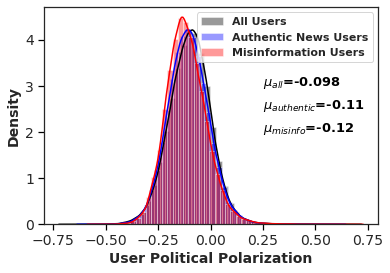
\includegraphics[width=1\linewidth]{figures/user_political_comparison.png}
      \caption{URL Set 1}
\label{fig:political-users1}
\end{subfigure}%s
\begin{subfigure}{.4\textwidth}
  \centering
  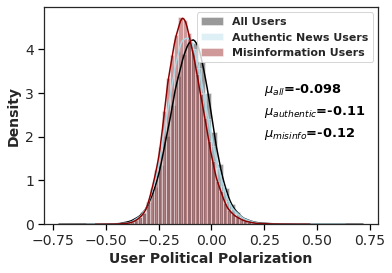
\includegraphics[width=1\linewidth]{figures/user_political_comparison2.png}
      \caption{URL Set 2}
  \label{fig:political-users2}
\end{subfigure}

\caption{\textbf{Political polarization of users who comment under authentic news and misinformation Reddit submissions}-- There are not significant differences in political ideology between users who comment on misinformation and those that comment on authentic news. }
\label{fig:users-political-orientation}
\end{figure*}
\begin{figure*}
\begin{subfigure}{.4\textwidth}
  \centering
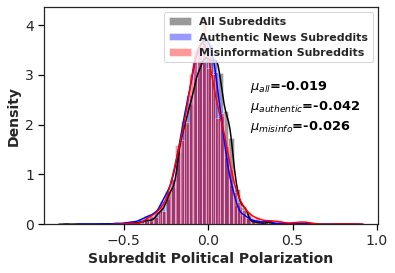
\includegraphics[width=1\linewidth]{figures/subreddit_political_comparison.png}
    \caption{URL Set 1}
\label{fig:harmonic-sub1}
\end{subfigure}%s
\begin{subfigure}{.4\textwidth}
  \centering
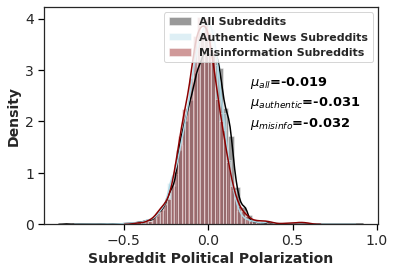
\includegraphics[width=1\linewidth]{figures/subreddit_political_comparison2.png}
    \caption{URL Set 2}
  \label{fig:pagerank-sub2}
\end{subfigure}

\caption{\textbf{Political polarization of subreddits with authentic news and misinformation Reddit submissions}--- There are no significant differences in the political orientation of subreddits where misinformation and authentic news appear. }
\label{fig:subreddit-misinformation-authentic-toxicity}
\end{figure*}
Looking at the set of users commenting under misinformation Reddit submissions, we surprisingly do not see dramatic differences between these users and those that comment on authentic news submissions. In fact, as seen in Figure~\ref{fig:users-political-orientation} for both our set of misinformation URL sets, we see a slight leftward tilt in the average commenter. Similarly and surprisingly, looking in Figure~\ref{fig:subreddit-misinformation-authentic-toxicity} at the political orientation of the subreddits where our misinformation submissions appeared, we again see that there is not much difference in their respective polarizations. This appears to indicate that \emph{both} misinformation and authentic news appear within subreddits and get commented on by users across the political spectrum.

%This indicates that the particular higher levels of toxicity observed in our set of misinformation-filled subreddits is not being driven by the political environment of the subreddit. 

We note that despite misinformation appearing in subreddits across the political spectrum, the users that post misinformation have a rightward tilt compared to the users that comment on misinformation. As seen in Figure~\ref{figure:misinformation-posters-commenters}, for both sets of URLs submissions with comments, we see that misinformation submitters are on the whole more conservative than their corresponding more liberal commenters. This is largely in contrast to authentic news commenters and posters. As seen in Figure~\ref{figure:news-posters-commenters}, authentic news posters and commenters share nearly the exact same distribution. 




\begin{figure}
\centering
\begin{subfigure}{.4\textwidth}
  \centering
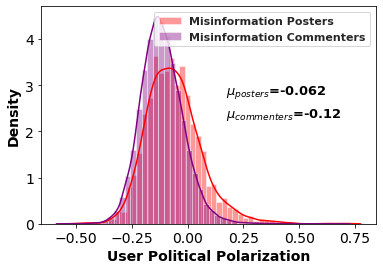
\includegraphics[width=1\linewidth]{figures/misinformation_posters_commenters.png}
    \caption{URL Set 1}
\end{subfigure}
\begin{subfigure}{.4\textwidth}
  \centering
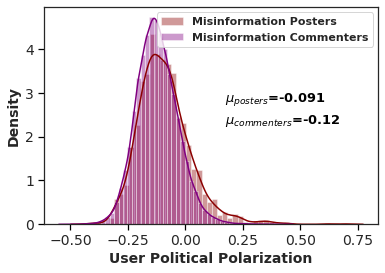
\includegraphics[width=1\linewidth]{figures/misinformation_posters_commenters2.png}
    \caption{URL Set 2}
\end{subfigure}
\caption{\textbf{Distribution of political orientation of posters and commenters of misinformation}--- There is a noticeable rightward tilt in users that post misinformation compared to those that comment on misinformation.}
\label{figure:misinformation-posters-commenters}

\end{figure}



\begin{figure}
\centering
\begin{subfigure}{.4\textwidth}
  \centering
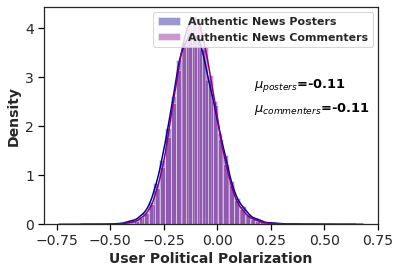
\includegraphics[width=1\linewidth]{figures/news_posters_comenters_comparison.png}
    \caption{URL Set 1}
\end{subfigure}
\begin{subfigure}{.4\textwidth}
  \centering
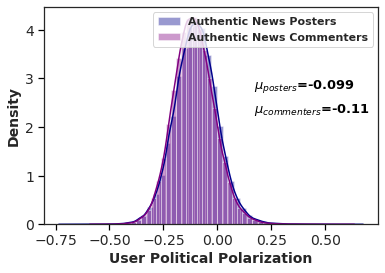
\includegraphics[width=1\linewidth]{figures/news_posters_comenters_comparison2.png}
    \caption{URL Set 2}
\end{subfigure}
\caption{\textbf{Distribution of political orientation of posters and commenters of authentic news}--- Unlike for misinformation posts, the posters and the commenters on authentic news share similar distributions of political orientations.}
\label{figure:news-posters-commenters}
\end{figure}

Altogether, we thus observe (especially in contrast to authentic news submissions), that a politically different set of users post misinformation news compared to those that comment on it. While we did not observe that the polarization levels of users who comment on misinformation are substantially different from commenters on authentic users, we did observe that they \emph{are} different from posters of misinformation content. 

\subsection{Intersection of Misinformation, News Media, Toxicity, and Political Polarization across Subreddits}
Finally, having seen the distribution of the political polarization and toxicity among different users and in different environments, we now look if these different characteristics correlate with the amount of misinformation and authentic news in each subreddit. Namely, we seek to determine more broadly if levels of misinformation are correlated with increased levels of toxicity. To do this we rely on our list of \textit{misinfo-oriented} and \textit{mainstream-oriented} websites.



Specifically, for each subreddit in our dataset, we compute their \textit{misinformation similarity} and their \textit{mainstream similarity} based on the percentage of each subreddit's  URL submissions that come from websites that are \textit{misinfo-oriented} and \textit{mainstream-oriented}. This measurement essentially determines the rough approximate percentage of submissions within each of our subreddits that are misinformation oriented/related and the percentage that are mainstream oriented/related. 

\begin{figure}
\begin{minipage}[l]{0.6\textwidth}
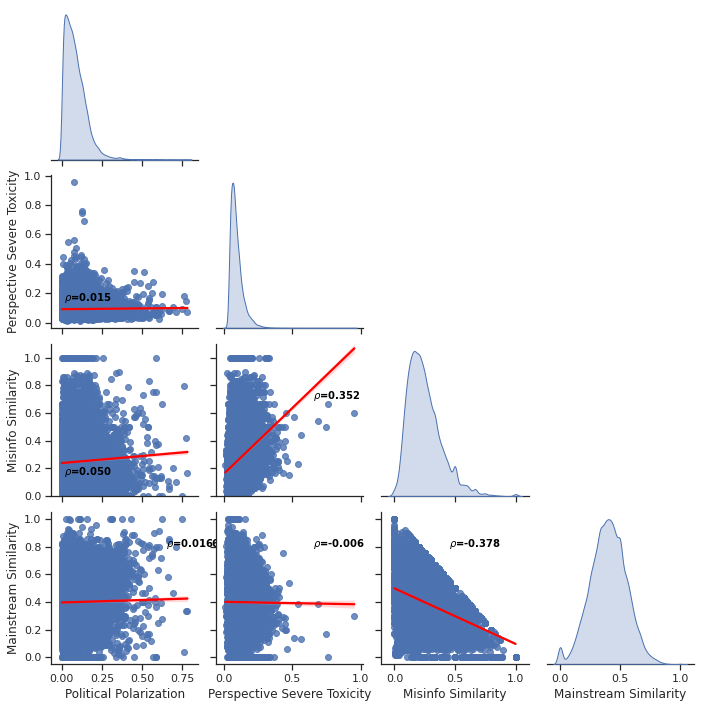
\includegraphics[width=1\columnwidth]{figures/cross_graphs.png} 
\end{minipage}
\begin{minipage}[l]{0.35\textwidth}
\caption{\textbf{Misinformation, toxicity, and political polarization interactions}--- As subreddits increase in misinformation levels, they become more toxic. However, there is not a large correlation between misinformation levels and the political polarization of subreddits. Similarly, we do not see any correlation between political polarization levels and mainstream similarity; nor do we see any correlation with toxicity levels.\label{figure:cross-graph} }
\end{minipage}

\end{figure}


As seen in Figure~\ref{figure:cross-graph}, across all our 46K considered subreddits, we observe that as subreddits become more similar to misinformation and hyperlink to more \textit{misinfo-oriented} domains, their toxicity increases. This largely matches our observation in Section~\ref{sec:toxicity} that misinformation submissions are in general more toxic/uncivil than authentic news submissions. Misinformation levels in general thus appear to be correlated with increased toxicity. We further again surprisingly see in Figure~\ref{figure:cross-graph} that levels of misinformation are not heavily correlated with political polarization. It does not appear that the most politically polarized environments necessarily rely upon misinformation. For example, the most left-leaning subreddits (Table~\ref{table:mostpolitical-subreddits}) that we observed mostly supported US Senator Bernie Sanders and did not necessarily have high misinformation levels. Conversely, we do not see much of a correlation between subreddits with high mainstream similarity and political polarization and toxicity. This again reinforces our results finding that mainstream news does not have higher levels of toxicity and political polarization level from Section~\ref{sec:toxicity} and Section~\ref{sec:polarization}. We thus see again from this analysis that misinformation is indeed correlated with higher toxicity, while authentic news is largely not. 
%\subsection{Reddit Level Interactions}
%Before examining the interaction directly within


\subsection{Summary}
In this section, we found that misinformation on Reddit largely is correlative with and predictive of higher amounts of incivility and toxicity on the platform. Most markedly, we observed that the comments under misinformation submissions are posted at a rate 60\% higher than the comments under authentic news submissions. Further, while we do observe a dichotomy in the political polarization of users that post misinformation and those that comment on misinformation, somewhat surprisingly, we find that misinformation appears across different political environments, with it not being concentrated just in the political extremes. Lastly, looking at how different levels of misinformation correlate with toxicity, we find the more \textit{misinfo-oriented} submissions a given subreddit has, the more toxic/uncivil it is likely to be. 

 
%\section{RQ2: Misinformation and Polarized Toxic Conversations}\label{sec:toxic-polarized-subreddits}
As seen in the previous section, comments are 60\% more toxic under misinformation submissions than authentic news submissions. Furthermore, there appears to be a difference in the political orientation of users that post misinformation and those that comment on it.  Given this difference and the higher toxicity levels present within misinformation submission comments, we now turn to understand if and how these \textit {political differences} drive toxicity within Reddit misinformation submissions. 

\subsection{Experimental Setup}
To fully understand how different levels of \textit{political differences} fuel toxicity and incivility, for this section, we reconstruct the conversational dyads that exist underneath each Reddit submission using the data provided by Pushshift~\cite{baumgartner2020pushshift}. Comments underneath Reddit submissions are similar to conversational threads; if a user responds to a given comment, their reply will appear underneath the comment. For each submission in our dataset, we thus determine using the thread information whether the commenter posted a response directly to another commenter. This then enables us to reconstruct conversational dyads between individual Reddit users. Then, using the approach outlined in Section~\ref{sec:reddit-methods}, we determine the polarization and average toxicity of the users in our conversational dyads. From these calculations, we further label users as conservative/conservative-leaning (positive polarization score) or liberal/liberal-leaning (negative polarization based). Lastly, looking at each of these conversational dyads, we determine if each user's response to each other is toxic/uncivil by utilizing the Perspective API SEVERE\_TOXICITY classifier with a cutoff of 0.8 (as also outlined in Section~\ref{sec:reddit-methods}). For a comparison of how conversations differ between misinformation and authentic news comments, we finally separate out the set of conversational dyads that appear under misinformation and authentic news submissions (for both sets of URLs). 
\begin{figure*}
\begin{subfigure}{.49\textwidth}
  \centering
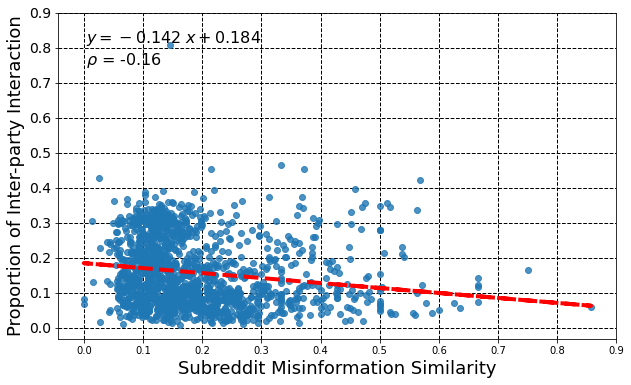
\includegraphics[width=1\linewidth]{figures/subreddit_interparty_interaction.png}

  \label{fig:pagerank-sub2}
\end{subfigure}
\begin{subfigure}{.49\textwidth}
  \centering
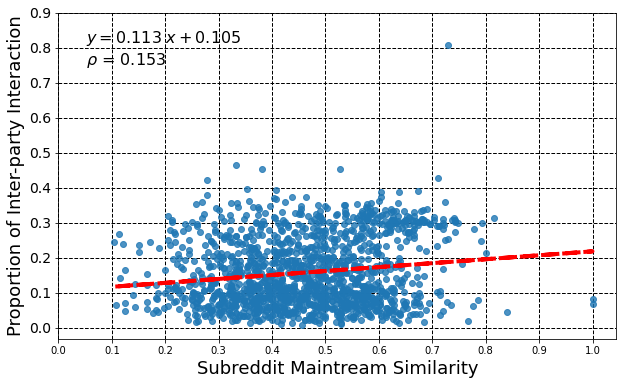
\includegraphics[width=1\linewidth]{figures/subreddit_mainstream_interaction.png}

  \label{fig:pagerank-sub2}
\end{subfigure}
\caption{\textbf{Proportions of inter-party interactions in different subreddits}---As subreddits hyperlink to more \textit{misinfo-oriented} websites, as a percentage, there are fewer and fewer interactions between conservative and liberal users. In contrast, there is a slight correlation between hyperlinking to \textit{mainstream-oriented} websites and more inter-party interactions. }
\label{fig:subreddit-misinformation-mainstream-similarity-interaction}
\end{figure*}




\subsection{Toxic Interactions within Misinformation and Authentic News Environments}
We find high amounts of homophily in interactions across our conversational dyads. Across all our conversational dyads, indeed 81.3\% of interactions are between users of the same political orientation (\textit{i.e} liberal-liberal, conservative-conservative). In contrast, for conversations under mainstream, and misinformation submissions, this increases to 81.7\% and 85.3\% respectively. We thus see slightly more conversational homophily within misinformation conversations than the entire Reddit population at large. Indeed using our set of \textit{misinfo-oriented} and \textit{mainstream-oriented} and looking at subreddits with at least 500 conversational dyads, as seen in Figure~\ref{fig:subreddit-misinformation-mainstream-similarity-interaction}, as website hyperlink to more \textit{misinfo-oriented} websites, conversations on their subreddits become more insular ($\rho =0.160$). In contrast, as subreddits hyperlink to more \textit{mainstream-oriented} websites, there is a slight increase in the amount of inter-party conversations ($\rho =0.153$). We thus see that misinformation is correlated with heightened political homophily within the subreddits, creating more insular communities, while authentic news is associated with a slight increase in political heterophily.

\begin{figure}
\centering
\begin{minipage}[l]{0.4\textwidth}
\centering
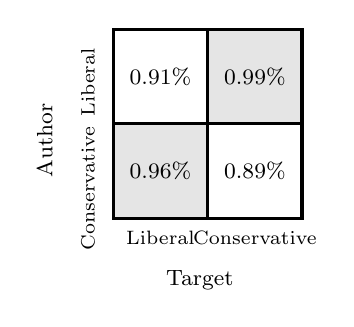
\begin{tikzpicture}[very thick]

    % Right square
    \node[fill=gray!20,draw=black, minimum size=1.2cm, inner sep=0pt] (as) {\footnotesize
$0.96\%$};
    \node[draw=black,minimum size=1.2cm, inner sep=0pt, above=-\pgflinewidth of as] (abh) {\footnotesize$0.91\%$};
    \node[draw=black,minimum size=1.2cm, inner sep=0pt, right=-\pgflinewidth of as] (abv) {\footnotesize$0.89\%$};
    \node[fill=gray!20,draw=black, minimum size=1.2cm, inner sep=0pt,  above right=-\pgflinewidth and -\pgflinewidth of as]  {\footnotesize$0.99\%$};
    
    % Side labels
    \node[anchor=east,rotate=90,yshift=0.3cm,xshift=0.7cm] at (as.west) {\scriptsize

Conservative};
    \node[anchor=north,] at (as.south) {\scriptsize
Liberal};
    \node[anchor=east,rotate=90,yshift=0.3cm,xshift=0.5cm] at (abh.west) {\scriptsize
Liberal};
    \node[anchor=north] at (abv.south) {\scriptsize
Conservative};
    
    
    % Square label
    \node[xshift=0.5cm, below=0.5cm of as] {\footnotesize Target};
    
    \node[yshift=1.0cm,xshift=-0.35cm,rotate=90,left=0.5cm of as] {\footnotesize Author};

\end{tikzpicture}
\end{minipage}
\begin{minipage}[c]{0.40\textwidth}
  \caption{\label{fig:interactions}\textbf{Percentage of interactions that are toxic/uncivil for authors and targets of different political leanings.} Across all 46K considered subreddits, there is a slight heterophily for users to reply in a toxic/uncivil manner to members with a tilt towards the opposite political party.}
\end{minipage}
\end{figure}    

Despite the increased political homophily within misinformation filled-subreddits, we observe a reverse trend in terms of toxic/uncivil comments. As seen in Figure~\ref{fig:interactions}, across all considered conversations, we see a slight heterophily for users to reply in a toxic/uncivil manner to users who are not of the same political leaning. We calculate an odds ratio of 1.17 for users to reply in a toxic manner to users of a different political leaning compared with users of the same political leaning. Comparing the set of toxic conversational dyads under misinformation submissions, we see an even higher heterophilic tendency. Compared with the baseline across all conversations, we observe a 25.2\% relative increase in the percentage of liberal to conservative toxic comments and a 12.5\% relative increase in the percentage of conservative to liberal toxic comments. In contrast, for authentic news submissions, we see a 23.2\% relative decrease in liberal to conservative toxic comments and an 18.8\% drop in the percentage of conservative to liberal toxic comments. This appears to indicate that while in misinformation-laced conversations, users are more likely to respond in a toxic manner to users of a different political orientation, users in authentic news-centered conversations are less likely.

To confirm, calculating the odds ratio we get 1.64 for misinformation toxic comments and  0.87 for mainstream toxic comments when comparing the percentages of politically heterophilic toxic comments to politically homophilic comments. Overall we thus find that on average, within misinformation submission comments that users are slightly more likely to respond with a toxic comment to users of different political leaning compared to all submissions on Reddit. This largely explains the higher levels of toxicity observed within misinformation submissions in Section~\ref{sec:toxicity} given the political differences we further observed between misinformation posters and misinformation comments.
 \begin{figure}
    \centering
    \begin{subfigure}{.4\textwidth}
       \centering
\begin{minipage}[c]{\textwidth}
   \centering
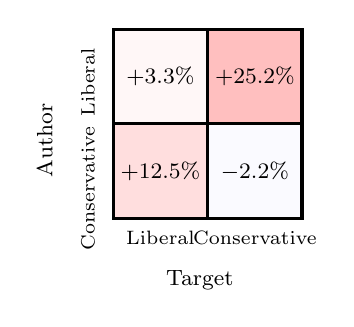
\begin{tikzpicture}[very thick]
    % Right square
    \node[fill=red!13,draw=black, minimum size=1.2cm, inner sep=0pt] (as) {\footnotesize$+12.5\%$};
    \node[fill=red!3,draw=black,minimum size=1.2cm, inner sep=0pt, above=-\pgflinewidth of as] (abh) {\footnotesize$+3.3\%$};
    \node[fill=blue!2,draw=black,minimum size=1.2cm, inner sep=0pt, right=-\pgflinewidth of as] (abv) {\footnotesize$-2.2\%$};
    \node[fill=red!25,,draw=black, minimum size=1.2cm, inner sep=0pt,  above right=-\pgflinewidth and -\pgflinewidth of as]  {\footnotesize$+25.2\%$};
    
   % Side labels
    \node[anchor=east,rotate=90,yshift=0.3cm,xshift=0.7cm] at (as.west) {\scriptsize

Conservative};
    \node[anchor=north,] at (as.south) {\scriptsize
Liberal};
    \node[anchor=east,rotate=90,yshift=0.3cm,xshift=0.5cm] at (abh.west) {\scriptsize
Liberal};
    \node[anchor=north] at (abv.south) {\scriptsize
Conservative};
    
    
    % Square label
    \node[xshift=0.5cm, below=0.5cm of as] {\footnotesize Target};
    
    \node[yshift=1.0cm,xshift=-0.35cm,rotate=90,left=0.5cm of as] {\footnotesize Author};


\end{tikzpicture}
\end{minipage}
   \caption{Misinformation Submission comments}
\end{subfigure}
\begin{subfigure}{.4\textwidth}
\begin{minipage}[c]{\textwidth} 
   \centering
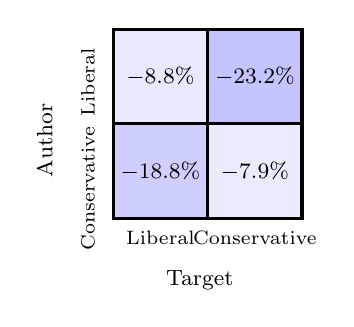
\begin{tikzpicture}[very thick]
    % Right square
    \node[fill=blue!19,draw=black, minimum size=1.2cm, inner sep=0pt] (as) {\footnotesize$-18.8\%$};
    \node[fill=blue!9,draw=black,minimum size=1.2cm, inner sep=0pt, above=-\pgflinewidth of as] (abh) {\footnotesize$-8.8\%$};
    \node[fill=blue!8,draw=blue!20,draw=black,minimum size=1.2cm, inner sep=0pt, right=-\pgflinewidth of as] (abv) {\footnotesize$-7.9\%$};
    \node[fill=blue!23,draw=black, minimum size=1.2cm, inner sep=0pt,  above right=-\pgflinewidth and -\pgflinewidth of as]  {\footnotesize$-23.2\%$};
  % Side labels
    \node[anchor=east,rotate=90,yshift=0.3cm,xshift=0.7cm] at (as.west) {\scriptsize

Conservative};
    \node[anchor=north,] at (as.south) {\scriptsize
Liberal};
    \node[anchor=east,rotate=90,yshift=0.3cm,xshift=0.5cm] at (abh.west) {\scriptsize
Liberal};
    \node[anchor=north] at (abv.south) {\scriptsize
Conservative};
    
    
    % Square label
    \node[xshift=0.5cm, below=0.5cm of as] {\footnotesize Target};
    
    \node[yshift=1.0cm,xshift=-0.35cm,rotate=90,left=0.5cm of as] {\footnotesize Author};

\end{tikzpicture}
 \caption{Authentic News Submission comments}
 \end{minipage} 
 \end{subfigure}
   \caption{Percentage increases of interactions that are toxic/uncivil in misinformation submissions for conservative and liberal authors against conservative and liberal targets.}
\end{figure}   

\subsection{Modeling toxic interactions between users commenting under Misinformation Submissions}
In order to confirm the finding that users of different political stripes in misinformation-laced conversations are more likely to reply in a toxic manner to each other, we fit our network data of toxic interactions to an exponential random graph model (ERGM). Exponential Random Graph Models (ERGM) is a form of modeling that predicts connections (toxic interactions) between different nodes (users) in a given network~\cite{hunter2008ergm}. ERGM models assume that connections are determined by a random variable $p^*$ that is dependent on input variables. As in Chen \textit{et al.}~\cite{chen2022misleading} and Peng \textit{et al.}~\cite{peng2016follower}, we utilize this modeling as it does it does not assume that its data input is independent; given that we want to model the interactions of polarization, toxicity, this relaxed restriction is key (we have already seen that they are largely not independent)~\cite{van2019introduction,hunter2008ergm}. Utilizing this framework, we thus model the probability of toxic interactions between a given author and target within misinformation submissions as a function of 1) their percentage of toxic comments, 2) their political polarization, 3) the difference in the author and target's political polarization 4) reciprocity between the author and target (\textit{i.e.} if the author and target both had a toxic comment aimed at each other), and finally 5) the number of subreddits that they share. 
\begin{table}[b]
\centering
\begin{tabular}{lr}
\toprule
   \multicolumn{2}{c}{\large Toxic Misinformation Submission Interactions}          \\
   \toprule
   & Coefficeint \\
      \midrule
      Intercept               &***-8.530 \\               
      \midrule
     Absolute User Polarization       &         -0.464 \\
      \midrule
      User Polarization Differences     & ***-0.782 \\
    \midrule
       User Toxicity &   ***12.396\\
      \midrule
       Reciprocity &  ***4.568\\
      \midrule
       Shared Subreddits &  0.00051\\
\bottomrule
 $\quad\quad\quad\quad ^\ast p<0.05; \;  ^{**} p<0.01; \; ^{***}p<0.001$ \\
\end{tabular}
\caption{As confirmed in our ERGM, differences in political orientation of users is predictive of increased incivility and toxicity. Similarly, the higher each individual user's toxicity norm they are more likely to target other users with toxic comments. }
\label{tbl:ergm}
\end{table}

Fitting our ERGM, we indeed find that as users become more politically distinct from each other, the more likely they are to target each other with uncivil or toxic comments (negative coefficient implies heterophily). As seen in Table~\ref{tbl:ergm}, political polarization by itself does explain toxicity as found by our model; rather differences between users seem to promote toxicity. This largely reinforces are findings from Section~\ref{sec:rq1}. Similarly, as expected, we find that higher levels of user toxicity norms and reciprocity between users are predictive of an increased probability of engaging in toxic interactions. We do not find as users share more subreddits that they are more likely to engage in toxic interactions with each other. 
We thus have seen that not only do misinformation submissions have more insular conversations, with 85.3\% of conversational dyads between users of the same political orientation (compared to 81.3\% of conversations under all Reddit submissions) but also that users become more hostile to users of the opposing political orientation.

\begin{figure*}
\begin{subfigure}{.49\textwidth}
  \centering
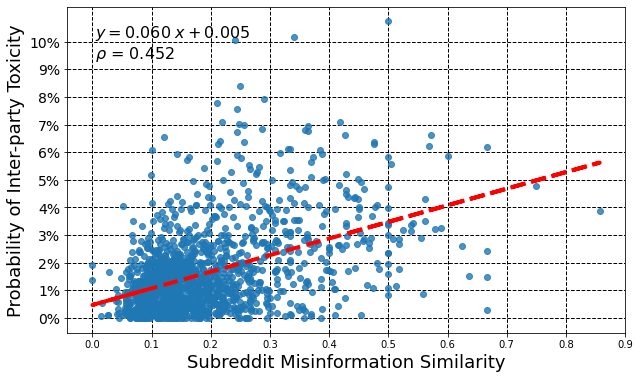
\includegraphics[width=1\linewidth]{figures/subreddit_misinformation_interparty.png}
\label{fig:misinformation-interparty}
\end{subfigure}%s
\begin{subfigure}{.49\textwidth}
  \centering
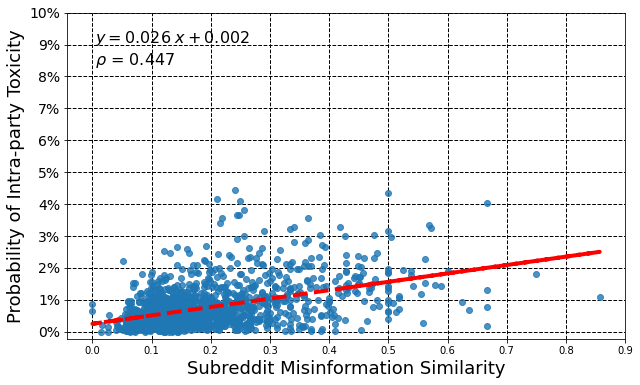
\includegraphics[width=1\linewidth]{figures/subreddit_misinformation_intraparity_toxicity.png}
  \label{fig:misinformation-intrapary}
\end{subfigure}

\caption{\textbf{Subreddit misinformation similarity vs. probability of toxic interactions between users of different and same political orientation}--- While for both inter-political and intra-political interactions, as misinformation similarity in a subreddit increases, the probability of a toxic interaction increases, for inter-political interactions the rate of increase is nearly double. }
\label{fig:subreddit-misinformation-rate-toxictiy-rate}
\end{figure*}


\subsection{Misinformation and increased rates of inter-political toxicity}
Finally, having confirmed that users posting under misinformation submission of different political orientations are more likely to engage in negative interactions with each other, we finally determine if the levels of misinformation within given subreddits as a whole leads to increased heterophilic toxic interactions. Namely as misinformation levels in a subreddit as a whole increase does the probability of negative interactions between users of different political orientations increase. We thus now plot the percentage of misinformation within a given subreddit against the probability of toxic interaction between members of the two political orientations. 


As seen in Figure~\ref{fig:subreddit-misinformation-rate-toxictiy-rate} looking at subreddits with more than 500 conversational dyads, we see that as subreddits have more \textit{misinformation-oriented} hyperlink submissions, the percentage of conversations dyads between users of different political leanings increases. Concretely, subreddit \textit{misinformation similarity} and the probability with which inter-political conversations are toxic have a correlation of $\rho=0.452$. While we similarly see that intra-political toxicity also increases with a similar correlation $\rho=0.447$, we see the rate at which misinformation induces inter-political toxicity is nearly 2.3 times that of intra-political toxicity (0.060 slope vs 0.026 slope). This reflects the fact that \textit{misinformation oriented} submissions are on the whole more toxic but that they increase politically heterophilic toxicity more than politically homophilic toxicity. 
\begin{figure*}
\begin{subfigure}{.49\textwidth}
  \centering
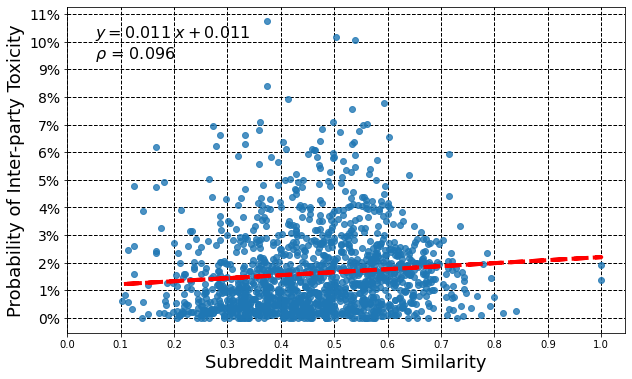
\includegraphics[width=1\linewidth]{figures/subreddit_mainstream_toxicity_interparty.png}
\label{fig:misinformation-interparty}
\end{subfigure}%s
\begin{subfigure}{.49\textwidth}
  \centering
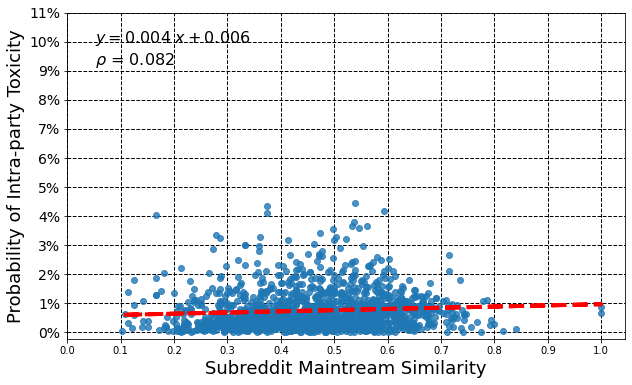
\includegraphics[width=1\linewidth]{figures/mainstream_intra_party_toxic.png}
  \label{fig:misinformation-intrapary}
\end{subfigure}

\caption{\textbf{Subreddit misinformation similarity vs. probability of toxic interactions between users of different and same political orientation}--- For both inter-political and intra-political interactions, as mainstream similarity in a subreddit increases the probability of inter- and intra-political toxicity is largely flat.}
\label{fig:subreddit-mainstram-rate-toxictiy-rate}
\end{figure*}

Again comparing against subreddit mainstream similarity, we do not see a similar relationship. As seen in Figure~\ref{fig:subreddit-mainstram-rate-toxictiy-rate}, the relationship between inter-political and intra-political toxicity rates and similarity to mainstream sources is largely flat. 


\subsection{Summary} Misinformation, we find, not only promotes higher levels of toxicity in general but also appears to drive inter-political incivility. Fitting an ERGM to our misinformation toxic dyads, we indeed find that political differences (along with reciprocity and each user's toxicity) are a driving force behind the formation of a toxic conversational thread. Finally, examining how different levels of misinformation promote toxicity among users, we find that across our considered subreddits, misinformation drives inter-political incivility at 2.3 times the rate of intra-political toxicity. 





















 





%We now seek gain an understanding of whether Reddit subreddits where the misinformation URLs  were posted or the users commenting in the submissions themselves were driving the toxicity within the misinformation submissions. As seen in Figure~\ref{}, misinformation subreddits in both 



    































%\section{RQ3: Engagement with Misinformation and Authentic News}
Having explored how misinformation on Reddit promotes toxic, insular, and polarized environments on Reddit, we finally turn to understand these factors' role in user engagement with misinformation and authentic news.  Namely having seen that misinformation produces more toxic and politically uncivil environments, do these environments lead to more engagement with misinformation? Various works have found that toxic and polarized environments often provoke engagement from users as they get ``outraged'' by the presented content~\cite{kim2021distorting,gallacher2021online}. In this final section, we seek to determine how different communities and different community norms affect the rates at which misinformation and authentic news get interactions on Reddit.

\subsection{Experimental Setup} To understand user interactions and engagement with misinformation and authentic news URL submissions, we utilize the number of comments that each submission receives. We utilize the number of comments rather than the number of upvotes/downvotes, due to the unreliability of Pushshift's data for this particular submission characteristic. While Pushshift often can acquire most submissions and comments, it often fails to keep up-to-date information about the number of votes a given submission receives~\cite{baumgartner2020pushshift}. This is largely due to the high rate at which submission upvotes/downvotes change. We thus use the more stable and reliable ``number of comments'' number to determine user engagement with a given submission. We lastly note that to properly model the number of comments, we remove comments from Reddit ``auto moderator'' accounts (often subreddits have auto moderators that automatically comment on submissions). We thus consider the number of comments from ``real world'' users. 

\begin{figure}
\begin{minipage}[l]{0.4\textwidth}
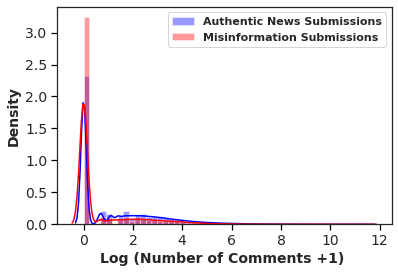
\includegraphics[width=1\columnwidth]{figures/num_submissions.png} 
\end{minipage}
\begin{minipage}[l]{0.35\textwidth}
\caption{\textbf{Log of number of submissions for misinformation and authentic news submissions}--- A large majority of submissions do not receive  comments.\label{fig:num_comments}}
\end{minipage}

\end{figure}


To model the count data of the number of comments on given submissions, we utilize a zero-inflated negative binomial regression~\cite{ridout2001score}. Within our regression, each observation represents a single submission and the number of comments it garnered. We specifically utilize a zero-inflated negative binomial regression as it appropriately models our set of count data. Unlike a Poisson model, which is often utilized to model count data, negative binomial regressions do not make the strong assumption that the mean of the data is equal to the variance~\cite{morina2022web}. Given that some submissions garner thousands of comments while others garner none, utilizing a Poisson model would be somewhat inappropriate. We further utilize the zero-inflated version of this regression given the heavy preponderance of submissions that do not receive any comments. After removing comments from auto moderators, as depicted in Figure~\ref{fig:num_comments}, 54.5\% of submissions within our dataset did not receive any comments. A normal negative binomial model would thus be unable the correctly model this behavior. 

\begin{table}[b]
\centering
\begin{tabular}{lll}
\toprule
   \multicolumn{3}{c}{\large Number of Comments on Misinfo Submissions}          \\
   \toprule
                                  & {Zero Inflated}  & {Negative Binomial }  \\
                      &       \footnotesize{negative coefficient = } &  \footnotesize{positive coefficient = }\\
                      &       \footnotesize{more likely to get comments} &  \footnotesize{more comments}\\
      \midrule
      Intercept              & 5.3146*** & 3.290***  \\               
      \midrule
      Absolute User Polarization               & -7.2400***  & -4.5838***  \\
      \midrule
      Absolute Subreddit Polarization              & 5.3818 &0.9658** \\
    \midrule
       Subreddit Toxicity & -2.5780***   & 5.3042*** \\
      \midrule
       User Toxicity &   -11.3991  *** &  -11.8022***\\
      \midrule
      Average Subreddit Comments &  -7.0379 *** & 1.0354***  \\
\bottomrule
& $^\ast p<0.05; \;  ^{**} p<0.01; \; ^{***}p<0.001$ \\
\end{tabular}
\caption{Fit of our zero-inflated negative binomial regression on the number of comments on our set of misinformation URL submissions across different subreddits.} 
\label{tbl:misinfo-fit}
\end{table}
\begin{table}[b]
\centering
\begin{tabular}{lll}
\toprule
   \multicolumn{3}{c}{\large Number of Comments on Authentic News Submissions}          \\
   \toprule
                            & {Zero Inflated}  & {Negative Binomial }  \\
                      &       \footnotesize{negative coefficient = } &  \footnotesize{positive coefficient = }\\
                      &       \footnotesize{more likely to get comments} &  \footnotesize{more comments}\\
      \midrule
      Intercept              & 3.7182***  &2.7577*** \\               
      \midrule
     Absolute User Polarization               & -2.7390***  & -3.0487 ***  \\
      \midrule
      Absolute Subreddit Polarization              & 5.9227*** &1.4898 *** \\
    \midrule
      Subreddit Toxicity & 6.1866***  & 13.1317*** \\
      \midrule
       User Toxicity &   -14.8969*** &  --8.0695***\\
      \midrule
      Average Subreddit Comments &  -6.4304*** & 0.6121***  \\
\bottomrule
& $^\ast p<0.05; \;  ^{**} p<0.01; \; ^{***}p<0.001$ \\
\end{tabular}
\caption{Fit of our zero-inflated negative binomial regression on the number of comments on our set of authentic news URL submissions across different subreddits.} 
\label{tbl:mainstream-fit}
\end{table}
Zero-inflated negative binomial regressions return two sets of coefficients. One set of coefficients, the zero-inflated coefficients, estimated using logistic regression, give the probability that the given submission would receive 0 comments as a function of the covariates. Positive coefficients for these zero-inflated coefficients indicate that increases in the predictor variable make a receiving 0 comment more likely. Thus the more negative a coefficient, the more the given covariate correlates with inducing at least 1 comment. The second set of coefficients, the negative binomial coefficients, model the number of comments as a function of the covariates. For these coefficients, positive coefficients indicate that the larger the corresponding covariate, the more comments that submission was likely to have received.  We thus, in our analysis, can understand how different covariates affect the probability that a given submission will receive \textit{any} comments \emph{and} how these same covariates affect the number of comments received. 

For data, we model the number of garnered comments for both our set of 47,822 misinformation submissions and 787,603 authentic news submissions. As factors influencing the number of comments, we utilize (1) the submitter's polarization, (2) the subreddit's polarization, (3) the toxicity norm of the subreddit, (4) the submitter's toxicity norm, and (5) the average number of comments with the subreddit the submission was posted in. 


\subsection{Results}  Before engaging in a thorough analysis of the fits of our zero-inflated negative binomials, we first perform a spot-check on the results. We ensure that the higher the average amount of comments in a given subreddit the more likely a submission is to get comments and that this average correlates with more comments on given submissions. In other words, we check that submissions in subreddits where users comment more, also received more comments. As seen in both Tables~\ref{tbl:misinfo-fit} and~\ref{tbl:mainstream-fit}, for both misinformation and authentic news Reddit submissions as the average number of comments in a particular subreddit increases, (1) the more likely a submission is to get comments at all and (2) the more comments it is likely to get. Having observed this behavior, we now move to examine the rest of the covariates within our fits. 

\paragraph{User Polarization} We observe similar behavior for the effect of the posting user political polarization on the number of comments that the submissions received. For both authentic news and misinformation submissions, we see that as the submission's submitter becomes more politically polarized (\textit{i.e.} moves to the political extremes on the political left or right), the more likely their posts are to receive comments. With zero-inflated coefficients of -7.24 for misinformation submissions and -2.74 for authentic news submissions, we see that this is particularly true for misinformation submissions. This largely agrees with prior work that has shown that highly polarized users are likely to provoke and garner comments on social media platforms~\cite{kim2021distorting,howard2019ira}

However, despite highly polarized users being able to attract at least one comment, we further observe that for both authentic news and misinformation submissions as the posting user becomes more politically polarized, the fewer comments their post is likely to receive. This appears to indicate that in the case of misinformation and authentic news submission, Reddit users are perhaps being ``turned off'' and engaging less with highly polarized users~\cite{hetherington2008turned}compared to more politically neutral users.

\paragraph{Subreddit Polarization} While we are unable to conclude using our model whether subreddit polarization has an effect on misinformation submissions, we find that for authentic news submissions the more politically polarized a subreddit is, the less likely anyone is to comment on authentic news submissions. This may indicate as a whole that authentic news submissions do not ordinarily get much traction on highly polarized subreddits. Rather, as documented by Wang \textit{et al.}~\cite{wang2021multi} subreddits like these often ignore more trustworthy sources. We thus find that the insular nature of more partisan subreddits may be inducing them to largely ignore authentic news submissions when they appear within their subreddit.
 
In contrast, for both misinformation and authentic news submissions, we find that as polarization goes up, the more comments given submissions are likely to garner. This reflects that \emph{when} authentic news and misinformation submissions are noticed, the more polarized the environment, the more users seem to comment and engage with submissions~\cite{kim2021distorting}.
 
\paragraph{Subreddit Toxicity}
Looking at the subreddit toxicity, we see a marked difference between authentic news submissions and misinformation submissions. We see, notably, for misinformation submissions, the more toxic a subreddit is, the more likely the submission is to get comments. In contrast, for authentic news submissions, the more toxic the subreddit, the more likely the submission is to not get any comments at all. This appears to reflect that authentic news submissions may often not have ``clickbait'' titles that induce readers to often angrily engage with  material~\cite{chen2015misleading,potthast2016clickbait}. In contrast, oftentimes misinformation websites often post inflammatory articles designed to engender angst in their readership. For example, with regards to the COVID-19 pandemic, the misinformation website infowars.com~\cite{starbird2018ecosystem}  recently published a report entitled \textit{``Wake Up! Even The Masks Made You Sick''!} As subreddits get more toxic, we thus see that their users are more likely to engage with articles such as this. 
 
Similar to polarization, for both misinformation and authentic news submissions, we find that as subreddit toxicity goes up, the more comments given submissions are likely to garner. This again reflects that \emph{when} authentic news and misinformation submissions are noticed, the more toxic the environment the more users seem to comment and engage with submissions. We thus see that though authentic news submissions are more often ignored in toxic subreddits when compared to misinformation, when they are noticed, toxic environments produce more engagement with both types of submission. 

\paragraph{User Toxicity}  Finally, looking at user toxicity, we see similar behaviors for both authentic news and misinformation submissions. Most notably, as users become more toxic for both misinformation and authentic news submission, the more likely they are to provoke at least one comment. We thus see that user toxicity is a means by which to gain engagement from posting news articles generally. However, again in both cases, we see that while user toxicity often provokes at least one person to react, we see that this toxicity, often does not lead to more comments on the whole. As found in prior work, toxic users, while often sparking retorts as other users become enraged, also create unhealthy, short, and otherwise bad conversational outcomes~\cite{saveski2021structure,kumar2021designing}. This result largely matches our definition of individual toxicity as comments that \textit{are likely to make one leave the discussion} from Section~\ref{sec:misinformation-defintion}. We thus as a whole see that as entire communities/subreddit becomes more toxic, they are more likely to engage with materials more thoroughly, but as individual users become more toxic, they are more likely to end and otherwise shorten conversations. 







%

 %Furthermore due to new restrictions placed on the Twitter API, we no longer will 




\section{Discussion}
In this work, we determined the correlation of different aspects of partisanship and affective polarization with toxicity at a user and topic-level on Twitter. We find, most notably, that users who are at the tail end of the political spectrum (very right-leaning or very left-leaning) \emph{are not} more likely to post toxic content; rather, we observe that users that engage with a wide variety of different politically aligned accounts center have a higher likelihood of tweeting toxic messages. Further, as users interact with or mention other users from a wider range of political ideologies, they are more likely to post toxic content. We similarly find that users who interact with other users who more regularly post toxic content are more likely to post toxic content themselves. 

Examining these phenomena from a topic level, we find that most heavily partisan topics \emph{are not} the most toxic. Rather, topics often have complex relationships with the partisanship of the users who tweet about them. While some topics become more toxic as more right-leaning/left-leaning users tweet about them, others become less toxic. However, as with individual users, we find that as users from a wider range of political ideologies tweet about a given topic, the more toxic that topic. Here we discuss some of the limitations and implications of our results:


\subsection{Limitations}
We acknowledge several limitations of this work. Given our use of GAMs to estimate the effect of partisanship and political diversity and our lack of ability to perform direct experiments, our findings are largely correlational. While they do buttress and support a large literature of similar results~\cite{barbera2014social,barbera2015tweeting,dagoula2019mapping,bail2018exposure} that have found causal results in some cases for increased polarization due to interaction with users of different political beliefs, we acknowledge that \emph{our} results are not causal. We further note that due to new restrictions placed on the collection of Tweets~\cite{Singh2023}, we can not continue to measure the toxicity of users and political topics, going forward.

This work largely focuses on US-based political polarization and ideologies. As a result, while applicable to dynamics for Twitter accounts on the US-political spectrum, our results do not necessarily apply to political conversations in different contexts. However, given access to Twitter or similar social media websites such as Meta's Threads, our study can be replicated in different cultural contexts.

Finally, as found early in our work in Section~\ref{sec:labeling-toxic}, different individuals and datasets have different metrics for toxicity. While our use of Perspective API's definition of toxicity is standard throughout the literature~\cite{kumar2021designing,rajadesingan2020quick,saveski2021structure}, we do base our DeBERTa-based model toxicity detection on this definition; we acknowledge that it may not take into account all perspectives on what constitutes toxic online content. 


\subsection{Tribal Tendencies, Affective Polarization, Online Toxicity, and Online Echo Chambers on Twitter}
As found by others, heated political conversations often elicit toxicity as people of differing views debate and discuss their differences~\cite{salminen2020topic}. We find that this discourse is related to increased toxicity on Twitter. The political diversity of those involved in a given Twitter conversation surrounding a given topic, at least in the short form of tweets, is correlated with affective polarization and toxic content. Adding nuance to previous studies of communities that have found that like-minded users gather and reinforce each other's views, creating toxic echo-chambers~\cite{cinelli2020echo,starbird2018ecosystem,gronlund2015does}. While users naturally often congregate and more heavily engage with users like themselves (assortativity coefficient of 0.266), showing that some echo chambers may exist on Twitter, when users exit these chambers and engage with other users of differing political views, we observe that this tends to create user conflict~\cite{guess2018avoiding}. This result reinforces De Francisci Morales {et~al.}'s~\cite{de2021no} finding that interactions among users on Reddit with different political orientations have increased negative conversational outcomes, showing that it occurs in platform-wide user interactions and discussions. Further indeed across all users, we find that as they increasingly interact with users of different partisanship, the frequency of toxicity increases (Figure~\ref{fig:toxicity_vs_mention-new}). While this feature of online conversation is not the dominant factor in engendering toxic content, with other factors like a user's previous behavior~\cite{levy2022understanding}, the age of their account, and the toxicity of other users also contributing to online toxicity, we note that this apparent ``tribal tendency'' appears both on a user and topic-level across Twitter and across multiple Twitter threads illustrating the robustness of this finding~\cite{mamakos2023social,de2021no}.  

%Namely, as also found by Mamakos et al.~\cite{mamakos2023social}, as users engage with users different from them and in a wider variety of political contexts, they tend to be more toxic. We further note that this result also reinforces De Francisci Morales {et~al.}'s~\cite{de2021no} finding that interactions among users on Reddit with different political orientations have increased negative conversational outcomes. 


\subsection{Hyperpartisan Users and Topics}
In contrast to some prior work~\cite{nelimarkka2018social},  we find that users and topics that are hyperpartisan (\textit{i.e.}, very left-leaning users or very right-leaning users) are not necessarily more toxic than less ideological users. Rather, we find these users tend to mostly associate and interact with other users who share similar political views ($\rho=0.605$) and as a result, do not necessarily have higher toxicity levels. As also found by Gr{\"o}nlund et al.~\cite{gronlund2015does}, because hyperpartisan users and topics often do not attract users of differing political views, we find that these users and topics tend to be less toxic than topics and users that interact with a wider range of the political spectrum (\textit{e.g.}, topics and users nearer to the political center). This result indicates that political echo chambers, where only left-leaning or right-leaning interact among themselves may be less conflict-oriented on Twitter. As a result, we argue that if social media companies like Twitter wish to expose their users to a wider range of political views without increasing conflict on their platforms, these users may be amenable to these opposing views if they come from others nearer to themselves on the political spectrum.


%\subsection{Toxicity } While our work does find evidence of th  Our work adds to the growing literature challenging the prevalence 

\subsection{Intra-Topic Partisanship over Time}
In Section~\ref{sec:changes}, we observed that the political orientation of users who discuss any particular topic often changes over time. These changes, often coinciding with changes in toxicity, also illustrate that the views expressed on Twitter about particular topics often change as different users enter or leave conversations. We argue that future analysis of topics and their spread on Twitter \emph{must} take into account user-level characteristics such as partisanship given that these values often reveal the nature of how users are addressing individual topics. For example, as seen in Section~\ref{sec:changes}, understanding that conversations surrounding ``Moscow Mitch'' had been taken up by increasingly right-leaning users reveals the penetration of this insult into more conservative circles. 

%\subsection{Verified Users Contribution to Toxicity}
%While we find that users who are verified are less likely to be toxic in their interactions on Twitter, we find conversely that as more verified users are involved in a particular topic, this coincides with the toxicity of that topic increasing. We hypothesize that topics, where many verified users are involved, are fairly high-profile attracting users from across the political spectrum and thus encouraging increased affective polarization. We leave it to future work to fully examine these dynamics. 




\subsection{Toxic Birds of Feather}
In addition to finding that the range of political views encountered by a particular user is predictive of toxicity, we further find that topics and users who interact with other toxic users are more likely to be toxic themselves. This again buttresses prior work from Kim {et~al.}, Kwon {et~al.}, and Shen {et~al.}  who all find that exposure to these negative conversations actually increases observers' tendency to also engage in incivility~\cite{kim2019incivility,kwon2017offensive,shen2020viral}. While not a new finding~\cite{kumar2023understanding}, this illustrates that reducing toxic content online may have other downstream benefits; by removing more instances of toxic content, other users may be less likely to engage in toxicity themselves further reducing the amount of toxic content. Given the existence of particular toxicity norms within communities Reddit~\cite{rajadesingan2020quick}, where toxicity is rarely seen among users and toxic comments are looked down upon, we argue that removing toxic content may have a compounding effect, greatly improving the overall health of online discourse.




\subsection{Implications for the Twitter/X Platform} Our work simultaneously finds that topics that engage with a wider set of politically aligned users and that users that engage in a wider array of different political discussions are more likely to tweet toxic messages. Namely, exposure on the Twitter/X platform to differing views may essentially be counterproductive to producing civil online discussions~\cite{bail2018exposure}.  Furthermore, this suggests that recent attempts to widen the range of political discussion on Twitter may have the additional effect of increasing online toxicity~\cite{hickey2023auditing}. As such, we argue that as Twitter continues to widen the political conversation on its platform, to also maintain low levels of toxicity additional moderation steps or additional practices should be taken to slowly introduce users to other accounts with different political beliefs to themselves should be taken as well~\cite{munson2010presenting}. This accords with the recommendations and findings of Mamakos et al.~\cite{mamakos2023social} who found that as Reddit users engage with users different from them and in a wider variety of political contexts, they tend to be more toxic. Given that Twitter users are not siphoned out into individual communities that they specifically join and thus more easily engage with polarizing content and users with whom they disagree across their topics of interest, we argue that building a means by which to engage in better conversations across political differences can reduce toxicity and friction on the platform. For example, as also argued by~\cite{nelimarkka2018social} including a wide and generalized view of particular topics could potentially reduce polarization. Indeed, as found in Section~\ref{sec:topic-level-gam}, while initially sparking more toxicity, as topics include a wider and wider berth of political perspectives and as more users join a topic, the toxicity of that particular topic decreases. 

%We further note that this result also reinforces De Francisci Morales {et~al.}'s~\cite{de2021no} finding that interactions among users on Reddit with different political orientations have increased negative conversational outcomes. 

%We similarly find several instances where users will simply @/mention verified users and begin toxicly tweeting at them. Given the high degree of these types of ``toxicity waves'' and that these waves largely seem to focus on verified users, we argue that Twitter/X should take additional steps to protect these users or alert them when such a toxicity wave is occurring. 



\subsection{Future Work}
This work centered around understanding factors that contribute to the toxicity levels of individual users and within particular topics on Twitter/X. However, we note that several of the techniques employed within this work can be extended and utilized beyond our study.

%\vspace{2pt}
%\noindent
%\textbf{Identifying Hate and Toxic Topic Waves} As seen in Section~\ref{sec:partisan-toxic}, utilizing our approach, we managed to identify various instances where accounts encountered toxic tweets aimed at them and centered around a particular topic. For instance, we identified 16 different waves aimed at Elon Musk; altogether we identified 1,923 similar ``toxicity waves'' aimed at 3,822 different accounts. We note that our DeBERTa-based model, which we open-source for study and use, can further enable others to continue this work without having to rely on making online and black-box queries to the Perspective API. In future work, we plan to better identify when users specifically attack particular accounts by training a model to predict the ``ATTACK ON AUTHOR'' task provided by Google Jigsaw~\cite{perspectiveapi} along with other metadata embedded within Twitter conversations. While not the focus on this particular work, we note that by being able to automatically identify potential ``toxicity waves'' against particular users, our work could be utilized to protect journalists, public officials, and vulnerable populations.

\vspace{2pt}
\noindent
\textbf{Identifying the Role of Partisanship and Polarization on Different Platforms} In this work, while we focus on Twitter, we note that our approach can largely be utilized on different social media platforms (\textit{e.g.}, Facebook, Reddit, \textit{etc...}) to identify the role of partisanship and political polarization. Unlike on Twitter, where a feed is curated for the user, Reddit user interactions, for instance, are largely determined by the into which the communities self-select. Previous work has shown that entire communities can engage in cross-partisan toxic behavior~\cite{efstratiou2022non}. Similarly Bail et~al.~\cite{bail2018exposure} find that simply following users and repeatedly seeing disagreeable content can increase polarization. As such, we plan to explore the robustness of our findings about ``tribal tendencies'' in different contexts and what best practices can be utilized to ameliorate these tendencies. 











%\section{Reddit Level Interactions}
As found in prior work, subreddits maintain particular levels of toxicity community norms~\cite{rajadesingan2020quick}. For example, as found by Rajadesingan \textit{et al.}, the subreddit WhiteRights had much higher tolerance for toxic content than the subreddits NeutralPolitics or AskEconomics. In this section, we analyze how distinctive political norms and toxicity levels within given subreddits contribute to levels of misinformation. 


In order to get an approximation of the levels of misinformation within a given subreddit we utilize a set of 157,605 \textit{misinformation-oriented} websites. We define \textit{misinformation-oriented} websites as websites that have more connections from our set of misinformation websites than from authentic news (i.e., the majority of a site's inward links in a domain-based graph are from misinformation websites. Websites that have been widely documented as spreading falsehood and conspiracy theories are included within this list including InfoWars and 8kun.top~\cite{hanley2022no,starbird2018ecosystem}.


As seen in Figure~\ref{figure:misinfo-toxciity-polarization}, there are political and toxicity norms across the spectrum, with polarization levels not being correlated levels of toxicity nor with misinformation levels. We see in particular that subreddits that are at the edge of political spectrum actually have some of the lowest average Perspective Toxicity scores and the lowest amounts of misinformation hyperlinks. We thus see at that at the edges of the political spectrum, where users are more isolated and insular that the overall levels of toxicity within the subreddit are not as high as those more ``moderate'' subreddits. This suggests that these cohesive communities where users are more similar to each other may producing the least amounts of bad behavioral outcomes. 


As seen in Figure~{}, toxicity the


\begin{figure}
\centering
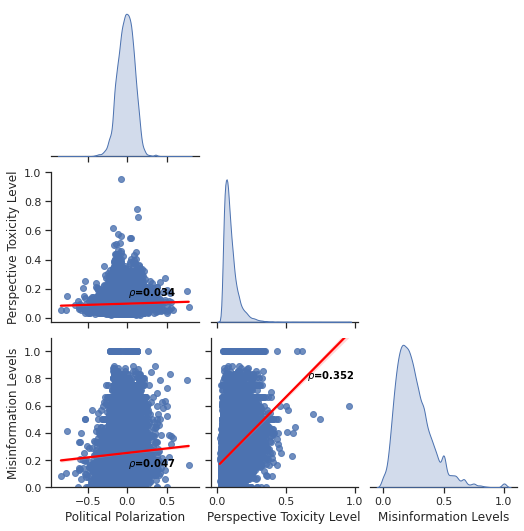
\includegraphics[width=0.75\columnwidth]{figures/subreddit_distribution.png} 
\caption{\textbf{Distributions of political polarization, perspective toxicity levels, and misinformation-oriented URL usage across subreddits with at least 100 users }--- While previous research has indicated that political polarization and toxicity are heavily correlated, we see in Reddit's case due to its self-selecting communities that political polarization is not correlated with vitriol and comment toxicity. Similarly we see that political polarization is not correlated with misinformation levels. Rather subreddits within the political center have the highest percentages of misinformation and toxicity. 
}
\label{figure:misinfo-toxciity-polarization}
\end{figure}
%\section{Borderless: Twitter Misinformation and Political Communities}
In this section, we analyze the interplay between the penchant towards political polarization, toxicity, and misinformation on social media users. Previous works have indicated that toxicity levels are heavily tied with users' political polarization levels~\cite{chipidza2021effect,kim2021distorting} as well as their penchant to conspiratorial content~\cite{hanley2021no}. We now investigate how toxic and political polarized communities contribute to the propagation of misinformation and conspiracies by individuals users on Twitter.  

\begin{figure}
\centering
\includegraphics[width=\columnwidth]{figures/LevelsOfMisinformationAndNewsOnTwitter.png} 
\caption{\textbf{Number of Authentic News, Misinformation, and Conspiracy Theory Links on Twitter in 2020}--- Misinformation maintains a large presence of Twitter, with about half as many links as authentic news. Conspiracy websites having a relatively small but non-negligible presence on the platform. 
}
\label{figure:levels_of_misinfo}
\end{figure}

As seen in Figure~\ref{figure:levels_of_misinfo}, counting the number of instances of misinformation, authentic news, and conspiracy theory hyperlinks based on a 1\% Twitter sampling over 6 months, there are consistent levels of misinformation news articles tweeted. The amount of misinformation links from users, in fact largely follows the amount of authentic news tweeted. Specifically, we find a Pearson correlation of 0.711 between the number of misinformation URLs posted and the number of authentic news posted.  At any given time, the amount of misinformation links within our dataset varies from, $\frac{1}{3}$ to $\frac{1}{2}$ of the amount of authentic news hyperlinks posted. Comparing this to a set of non-news related URLS as well as a set of random domains (chosen randomly from the Amazon Alexa Top 1M from January 1 2022), we see that the changing amounts of misinformation and news based URLs in our dataset is largely due to the vicissitudes of the news cycles rather than as an artifact of our dataset. 

Having established the relative levels of misinformation on Twitter, we now seek to understand some of the drivers behind misinformation heavy Twitter accounts. Taking all URLS within our dataset, we acquire 189K different Twitter accounts that tweets authentic news, misinformation, or conspiracy theories during the month of January. Within this set of Twitter accounts 139663 accounts tweeted at least one authentic news website and 115073 accounts tweeted at least one misinformation website. Using the Tweepy API, we collect the last 3240 tweets of each of these users, giving us a dataset of 446,439,819 tweets total. 

\begin{figure*}
\begin{subfigure}{.25\textwidth}
  \centering
  \includegraphics[width=1\linewidth]{figures/all-correlations.png}
  \caption{All User Correlations}
\label{fig:twitter-reddit-partisanship-time}
\end{subfigure}%
\hspace{20pt}
\begin{subfigure}{.25\textwidth}
  \centering
  \includegraphics[width=1\linewidth]{figures/republican-correlations.png}
  \caption{Republican User Correlations}
  \label{fig:twitter-reddit-partisanship}
\end{subfigure}
\hspace{20pt}
\begin{subfigure}{.25\textwidth}
  \centering
  \includegraphics[width=1\linewidth]{figures/democratic-correlations.png}
  \caption{Democratic User Correlations}
  \label{fig:twitter-reddit-toxicity-time}
\end{subfigure}
\caption{\textbf{Twitter User Characteristic Correlations}--- Among different 
}
\label{fig:twitter-correlations}
\end{figure*}

After labeling each tweet with the Perspective API and gathering each accounts approximate partisanship, partisanship URL variance, and misinformation promotion levels, we now seek to understand the factors behind accounts promoting misinformation. As a proxy for the misinformation promotion level of given Twitter users, we utilize the percentage of the URLs that they post that belong to our set of misinformation domains.

As seen in Figure~\ref{fig:twitter-correlations}, there is a high degree of correlation between the political polarization of users and misinformation levels of users. This largely concurs with prior research that suggests that political polarization is the most potent reason behind the sharing of ``fake-news'' on Twitter~\cite{osmundsen2021partisan}. Looking at users whose average URL posted is conservative/Republican, this is especially prominent,  with polarization having a 0.70 Pearson correlation with levels of misinformation on their accounts. 


We also see, somewhat counter-intuitively, at a given level of partisanship, as the partisanship variance of individuals accounts increases, the amount of misinformation that that account post also increases. This suggests that users that actually engage with materials/hyperlink to materials that are substantially different from the average political information that they hyperlink to are more likely to post misinformation. Bucking our initial expectations, engaging with more and different sources is associated with heavier amounts of misinformation. Prior work~\cite{starbird2018ecosystem} has noted the political echo chambers that promote misinformation online. However, this appears to be only a part of the story of the spread of misinformation. 
\begin{comment}
\begin{figure}
\centering
\includegraphics[width=\columnwidth]{figures/misinformation-graph-partisan-var.png} 
\caption{\textbf{Partisanship and Partisanship Variance Affect on Misinformation}--- As users become more politically hardened and engage with a higher amount of news sources, they are more likely to post misinformation. While not exact, as levels of variety of political URLS posted increases at each level of partisanship, the the levels of misinformation increases as well. This is seen by the red fraying at the edges of the graph.  
}
\label{figure:partisanship-misinfo-variance}
\end{figure}
\end{comment}
As seen in Figure~\ref{figure:partisanship-misinfo-variance}, it is the set of users that have the highest variance of political URLs as well as the most highly partisan users that have the highest levels of misinformation on their Twitter accounts.For example one particularly highly misinformation-dense account (Figure~\ref{fig:twitter-misinformation2}) linked to a video from MSNBC to deride one of its hosts. This is not to say that these users regularly link to highly opposing views often; however, this tendency to interact with substantially different than a user's political average results in a higher likelihood of misinformation. 
\begin{figure*}
\begin{subfigure}{.48\textwidth}
  \centering
  \includegraphics[width=1\linewidth]{figures/liberal-graph-partisan-misinformation.png}
\label{fig:left-twitter-pol-toxicity}
\end{subfigure}%
\begin{subfigure}{.48\textwidth}
  \centering
  \includegraphics[width=1\linewidth]{figures/conservative-graph-partisan-misinformation.png}
  \label{fig:right-twitter-pol-toxicity}
\end{subfigure}
\caption{\textbf{Average Misinformation Levels as a function of average political bias and tendency to post opposing views}-- Users that post the URLs of websites that are against their average political bias are more likely to post misinformation.
}
\label{fig:twitter-pol-toxicity}
\end{figure*}

Users that post more URLs that are opposed to their mean political URLs/belief also show a higher probability of toxicity compared to other users of similar political averages. Plotting levels of toxicity as a function of political bias and the tendency to post opposing views (URLs from websites that are conservative-leaning for Democratic voters and vice versa), we see 1) that levels of toxicity are highly connected with levels of partisanship ( Pearson correlation of 0.38 for all users), and 2) that as the number of URLs from websites with opposing views increases, we see that average levels of toxicity increase as well. Looking at Figure \ref{fig:twitter-pol-toxicity} and , we  that for both left-wing and right-wing users, similarity at each given partisanship level, as the percentage of URLs from websites that oppose their mean political bias increases, that mean levels of toxicity increases with users at the end of each level of partisanship showing the highest levels of toxicity. For liberal leaning users, we find that after normalizing for partisanship, a Pearson correlation of 0.242 between the average toxicity of a user and their tendency to post URLs opposing their political bias. Just looking at decidedly conservative users with an average political bias of 0.1 or greater, this correlation increases to 0.302. For conservative users, we find that after normalizing for partisanship, the tendency to post opposing views accounts, has a Pearson correlation of 0.240 with their average toxicity. Just looking at decidedly conservative users with an average political bias of 0.1 or greater, this correlation increases to 0.302. As seen, users with the tendency to post URLS against their political bias have higher associated levels of toxicity. This largely mirrors  the tendency to also post misinformation as previously discussed. 

\begin{figure*}
\begin{subfigure}{.3\textwidth}
  \centering
  \includegraphics[width=1\linewidth]{figures/high-var-user-tweet1.png}
\label{fig:twitter-misinformation1}
\end{subfigure}%
\begin{subfigure}{.3\textwidth}
  \centering
  \includegraphics[width=1\linewidth]{figures/high-var-user-tweet2.png}
  \label{fig:twitter-misinformation2}
\end{subfigure}
\begin{subfigure}{.3\textwidth}
  \centering
  \includegraphics[width=1\linewidth]{figures/high-var-user-tweet3.png}
  \label{fig:twitter-misinformation3}
\end{subfigure}
\caption{\textbf{Examples of partisan users engaging with material from across the political aisle }-- Highly partisan and misinformation dense Twitter accounts occasional respond to and engage with news stories from authentic news. As pictured, users often deride these sources or cite that stories are  highly divisive.
}
\label{fig:twitter-misinformation-levels}
\end{figure*}

%% Likelihood to post a right-leaning URL if left wing vs probability to post a left-wing URL if right leaning as a function of partisanship 
\begin{figure*}
\begin{subfigure}{.24\textwidth}
  \centering
  \includegraphics[width=1\linewidth]{figures/republican-democratic-graph.png}
  \caption{Partisanship Levels}
\label{fig:twitter-average-partisanship}
\end{subfigure}%
\begin{subfigure}{.24\textwidth}
  \centering
  \includegraphics[width=1\linewidth]{figures/partisan-variance-graph.png}
  \caption{Partisanship Variance}
  \label{fig:twitter-variance-partisanship}
\end{subfigure}
\begin{subfigure}{.24\textwidth}
  \centering
  \includegraphics[width=1\linewidth]{figures/toxicity-graph.png}
  \caption{Perspective Toxicity }
  \label{fig:twitter-toxicity}
\end{subfigure}
\begin{subfigure}{.24\textwidth}
  \centering
  \includegraphics[width=1\linewidth]{figures/misinformation-graph.png}
  \caption{Misinformation }
  \label{fig:twitter-misinformation}
\end{subfigure}
\vspace{5pt}
\caption{\textbf{Interconnections between Twitter users with corresponding levels of partisanship, levels of sharing differently partisan sourced articles, toxicity, and levels of misinformation }-- As seen in the above graphs, highly conservative/Republican users and highly democratic/Republican users largely reference each other. Among these highly polarized communities, these users share more disparate and polarized articles, spread more misinformation, and are more toxic.
}
\label{fig:graph-correlations}
\end{figure*}

The tendency of user with higher levels of toxicity, higher levels of partisanship, and higher likelihoods to post misinformation further carries over to Twitter communities that many of these users participate in. Looking at the set of Twitter users in our scrape that posted at leas 300 URL (top 30K users in our dataset), we see this distinction visually. We plot Twitter mention graphs with edge weights based on how often each user mentions other users in their Tweets. Based on how often each user mentions another and clustering the graph using the Force Atlas 2 algorithm, we see two distinctive clusters of conservative/Republican and liberal/Democratic users form. As seen in Figure~\ref{fig:twitter-average-partisanship}, highly partisan users largely group and interact together, with conservative users mentioning other conservative users more frequently and vice versa. Looking a homophily (the tendency of users to mention/reference users of similar political bias as themselves) we see a moderately high value of 0.604. Comparing the graphs, in


As seen in Figure~\ref{fig:graph-correlations}, the cluster of highly liberal/Democratic and highly conservative/Republican users (Figure ~\ref{fig:twitter-average-partisanship}) corresponds to the set of users with higher amounts of political variance in the URLs that they tweet (Figure ~\ref{fig:twitter-variance-partisanship}) as well as the higher amounts of misinformation (Figure ~\ref{fig:twitter-misinformation}).

Looking at the graph of partisanship variance and the the graph of partisanship levels in Figure~\ref{fig:graph-correlations}, and the corresponding levels of correlation in between partisanship and partisanship variance, the most highly partisan accounts are the ones that hyperlink to a variety of different sources. This is particular true of Republican/conservative users. This can be most clearly seen in the dark pink cluster of the partisanship variance graph corresponding heavily with the Conservative/Republican red of the partisanship levels cluster, and finally dark orange cluster of the misinformation graph. 

%\section{Moderating Influences: Community Based Control on Misinformation Spread}
In this section, we examine the different misinformation ecosystems on Reddit. Largely in contrast to the self-organizing and porous communities that exist on Twitter, Reddit allows users to  establish their own self-contained communities. These communities known as subReddits have their own rules, communities norms, political preferences, as well as purposes. These subReddits module, control, and filter the content on Reddit platform. Behaviors in one subReddit that blocked or condemned in one subReddit can be widely celebrated in another subReddit. For example, one subReddit \texttt{r/conspiracy} that has over 1.7M (at time of writing in February 2022)  is dedicated to the discussion on conspiracy theories. Conspiracy Theories that are widely discussed in this subReddit are often ridiculed in other subReddit like \texttt{r/Qult\_Headquarters}.
\begin{figure*}
\begin{subfigure}{.48\textwidth}
  \centering
  \includegraphics[width=1\linewidth]{figures/average-toxicity-end-2020.png}
\label{fig:cdf-subreddit-hyperlinks}
\end{subfigure}%
\begin{subfigure}{.48\textwidth}
  \centering
  \includegraphics[width=1\linewidth]{figures/average-toxicity-distribution-end2020.png}
 \label{fig:cdf-user-hyperlinks}
\end{subfigure}
\label{fig:cdf-hyperlinsk}
\caption{\textbf{Relative Perspective API toxicity of tweets and comments on Twitter and Reddit}--- Comparing a 1\% Twitter stream's Perspective API toxicity scores to the bulk of Reddit comments from  July to December 2020, we see that Reddit has maintained lower levels of toxicity over time and amongst users. }
\end{figure*}


\begin{figure*}
\begin{subfigure}{.48\textwidth}
  \centering
  \includegraphics[width=1\linewidth]{figures/polarization_redidit_twitter.png}
\label{fig:cdf-subreddit-hyperlinks}
\end{subfigure}%
\begin{subfigure}{.48\textwidth}
  \centering
  \includegraphics[width=1\linewidth]{figures/average-toxicity-distribution-end2020.png}
 \label{fig:cdf-user-hyperlinks}
\end{subfigure}
\label{fig:cdf-hyperlinsk}
\caption{\textbf{Relative Perspective toxicity of tweets and comments on Twitter and Reddit}--- Comparing a 1\% Twitter stream's Perspective API toxicity scores to the bulk of Reddit comments from  July to Decemebr 2020, we see that Reddit has maintained lower levels of toxicity over time and amongst users. }
\end{figure*}
As seen in Figures~\ref{}

Because of self-organizing and fairly norm-heavy communities form on Reddit, we find that our set of misinformation URLs are largely confined to a small set of subReddits and set of users. As seen in Figure~\ref{fig:cdf-subreddit-hyperlinks}, fairly few subReddits are responsible for the amount of Misinformation URLs Reddit Submissions. For instance, we find that only 133 Reddits were responsible for 90\% of Misinformation URL submission on Reddit from July 2020 to December 2020. Only 4007 contained misinformation URLS within their submissions. 4878 different subReddits contained misinformation URLs in their comments.While some of misinformation posts could have been removed by moderators and Reddit itself, this illustrates the moderating effect community norms have on the material that is posted and stays posted in  the majority of subreddits. This is largely in contrast to the number of subReddits containing authentic news URLs, with 513 subReddits containing 90\% of authentic news URL submissions and 12,825 containing authentic news Reddit Submissions. 18131 different subReddits had authentic news domain hyperlinks in their comments from July 2020 to December 2020. This behavior among subreddits largely caries over to the set of Reddit users who posted these links to misinformation and authentic news websites. As seen in Figure~\ref{fig:cdf-user-hyperlinks}, just 1423 users were responsible for 90.0\% of of misinformation URLs subReddit submissions in contrast to the 11,336 responsible for authentic news submissions. 
\begin{figure*}
\begin{subfigure}{.48\textwidth}
  \centering
  \includegraphics[width=1\linewidth]{figures/misinformation-authentic-cdf.png}
  \caption{\textbf{CDF News Hyperlinks by Subreddit}— Just 133 subreddits posted  90.0\% of hyperlinks to the misinformation websites in our dataset from July 2020 to December 2020. In contrast, 513 subReddits posted 90.0\% of the hyperlinks to authentic news websites during this same period. 
}
\label{fig:cdf-subreddit-hyperlinks}
\end{subfigure}%
\begin{subfigure}{.48\textwidth}
  \centering
  \includegraphics[width=1\linewidth]{figures/misinformation-authentic-users-cdf.png}
 \caption{\textbf{CDF News Hyperlinks by User}— Just 1423 subreddits posted  90.0\% of hyperlinks to the misinformation websites in our dataset from July 2020 to December 2020. In contrast, a whopping 11,336 subReddits posted 90.0\% of the hyperlinks to authentic news websites during this same period. 
}
 \label{fig:cdf-user-hyperlinks}
\end{subfigure}
\label{fig:cdf-hyperlinsk}
\end{figure*}


\begin{figure*}
\begin{subfigure}{.48\textwidth}
  \centering
  \includegraphics[width=1\linewidth]{figures/partisanship_avg.png}
 
\label{fig:partisanship-average}
\end{subfigure}%
\begin{subfigure}{.48\textwidth}
  \centering
  \includegraphics[width=1\linewidth]{figures/toxicity_avg.png}
 
 \label{fig:toxicity-average}
\end{subfigure}
\begin{subfigure}{.48\textwidth}
  \centering
  \includegraphics[width=1\linewidth]{figures/partisanship_variance.png}
 
\label{fig:partisanship-variance}
\end{subfigure}%
\begin{subfigure}{.48\textwidth}
  \centering
  \includegraphics[width=1\linewidth]{figures/toxicity_variance.png}
 
 \label{fig:toxicity-variance}
\end{subfigure}
\caption{\textbf{Toxicity and Political URL Variation among Users and SubReddits }--- As seen above, there are relatively tight windows of political partisanship and toxicity among subreddits with subreddits having approximately little more diversity than individual users. 
}
\label{fig:diversity-of-views}
\end{figure*}
\begin{figure*}
\begin{subfigure}{.48\textwidth}
  \centering
  \includegraphics[width=1\linewidth]{figures/numberOfSubRedditsByPartianshipAvg.png}
  \caption{\textbf{User SubReddit Paritipation vs Variance in Political URLs Posted}-
}
\label{fig:participation-political}
\end{subfigure}%
\begin{subfigure}{.48\textwidth}
  \centering
  \includegraphics[width=1\linewidth]{figures/numberOfSubRedditsByToxicityAvg.png}
 \caption{\textbf{User SubReddit Paritipation vs Variance in Comment Toxicity}— 
}
 \label{fig:participation-toxicity}
\end{subfigure}
\caption{\textbf{Relative amounts of partisanship and toxicity diversity among individual users by SubReddit participation }--- As users participate in more and more the variance of their behavior increases with user posting a wider variety of political websites and commenting with a wider berth of toxicity. 
}
\label{fig:participation}
\end{figure*}
The moderating effect of subReddits is further seen in the relatively narrow window of political views and level of toxicity that are allowed within each subReddit community. As seen in Figure~\ref{fig:diversity-of-views}, there relatively narrow windows of allowed divergence in political beliefs and toxicity among SubRedits and users. This is in Figure~\ref{fig:participation}, as only as users participate in more and more subReddits does the berth of different types of comments that they post increase. On average, after a user participates in TODO subreddits the variance of their toxicity exceeds the average subReddit (an entire community). This illustrates the ability of subReddit communities to maintain an equilibrium of acceptable toxicity on their platforms, excising redditors who go outside normal bounds as illutrated in prior work~\cite{rajadesingan2020quick}.  Similarly, we find  that as users participate and post in more subReddits, they post a wider political range of websites.


\begin{figure*}
\begin{subfigure}{.48\textwidth}
  \centering
  \includegraphics[width=1\linewidth]{figures/user-partisanship-var.png}
  \caption{\textbf{Number of SubReddit Users vs Variance in Political URLs Posted}-
}
\label{fig:participation-political}
\end{subfigure}%
\begin{subfigure}{.48\textwidth}
  \centering
  \includegraphics[width=1\linewidth]{figures/user-toxicity-var.png}
 \caption{\textbf{Number of SubReddit Users vs Variance in Comment Toxicity}— 
}
 \label{fig:participation-toxicity}
\end{subfigure}
\begin{subfigure}{.48\textwidth}
  \centering
  \includegraphics[width=1\linewidth]{figures/partisanship-to-num-subreddits.png}
 
\label{fig:particiption-median-toxicity}
\end{subfigure}%
\begin{subfigure}{.48\textwidth}
  \centering
  \includegraphics[width=1\linewidth]{figures/toxicity-to-num-subreddits.png}

 \label{fig:cdf-user-hyperlinks}
\end{subfigure}
\label{fig:cdf-hyperlinsk}
\caption{\textbf{Number of Users to Variance in SubReddit Behavior}--- As the number of users in a particular subReddit increases, there is no discernible trend in the the variance of political URLS posted nor the Perspective API toxicity. However, as the the number of subReddits that the median user participates in increases within a given subReddit, the variance in political URLs and the the variance in toxicity does increase.  
}
\label{fig:participation}
\end{figure*}

Conversely, we find that the number of users that a subReddit contains, does not correlate with the diversity of toxicity and political views present on that subReddit. As seen in Figure~\ref{fig:participation}, as the number of users that post submissions in a subReddit increases, there is no discernible correlation with the variance of toxicity nor the variance of political views voiced on that subReddit. In contrast, we find that as the median subReddit participation on Reddit increases, the variance of toxicity and political viewd does increase.  Namely, if a subReddit has users that participate in a wide range of subReddits outside that particular subReddit, then this particular subReddit has higher levels of variance in political views and toxicity. This suggests that amount of people that a subReddit does not correspond with diversity of views and behavior on that subReddit but rather with the amount of communities that that subReddit's users come from and with which they engages. 
\begin{figure*}
\begin{subfigure}{.48\textwidth}
  \centering
  \includegraphics[width=1\linewidth]{figures/user-misinfo-toxicity.png}
\label{fig:user-misnformation}
\end{subfigure}%
\begin{subfigure}{.48\textwidth}
  \centering
  \includegraphics[width=1\linewidth]{figures/reddit-misinfo-toxicity.png}
 \label{fig:reddit-misinformation}
\end{subfigure}
\label{fig:misinformation-reddit-user}
\end{figure*}
Having established how the characteristics of subReddits exerts norms over their particular users, we now turn to understand how these norms affect the levels of misinformation on Reddit platform and on particular subReddits. 
As seen in Figure~\ref{fig:misinformation-reddit-user}, as on Twitter, misinformation subReddits as well as have higher levels of toxicity compared with subReddis with not misinformatino submissions. 

Looking a






\section{Conclusion}
In this work, we analyzed what factors potentially contribute to 
why users post toxic content on Twitter. We propose and implement a new open-source toxicity classifier, achieving better accuracy than the Perspective API on the Civil Comments dataset.  Then, analyzing 89.6M tweets posted by 43.1K users from across the political spectrum, we find a user or topic being heavily partisan does not necessarily imply increased toxicity; rather as users engage with and as conversations involve a wider range of political orientations and with other toxic users and toxic content that online toxicity increases.

%%
%% The acknowledgments section is defined using the "acks" environment
%% (and NOT an unnumbered section). This ensures the proper
%% identification of the section in the article metadata, and the
%% consistent spelling of the heading.


%%
%% The next two lines define the bibliography style to be used, and
%% the bibliography file.
\bibliographystyle{ACM-Reference-Format}
\bibliography{sample-base}

%%
%% If your work has an appendix, this is the place to put it.
\appendix
\section{Correspondence Analysis for Approximating Political Ideology\label{sec:appendix-ca}}
After identifying our set of 882 politically discriminating and identifying 7,7 random accounts that followed this set of accounts, we performed the following for CA. 

\begin{enumerate}
\item{\textbf{Identify the Ideological Subspace:}} Using 6,107 accounts that followed 10 or more of our 882 discriminating political users, we derive an initial CA model and obtain a discriminating latent space on which to plot user political ideology. 

\item{\textbf{Expand the number of discriminating political ideological accounts:}} Utilizing our initial CA model we determine the set of Twitter accounts not included within our initial target accounts that were most often followed by the most conservative and liberal accounts (within the top 20\% on either side of the political spectrum) in the first stage of our analysis. As in Barbera et~al.~\cite{barbera2015tweeting}, we compute the popularity among users of a given ideological orientation such that $pop_{jc} = n_{jc} -  n_{jl}$  for conservatives, where $n_{jc}$ is the number of conservative users included in the first stage
that follow account j, and $n_{jl}$ is the equivalent measure for liberals. We further filter these accounts to ensure that at least 3r different users follow these additional discriminating accounts. After determining these users, we add the resulting 788 accounts as additional "following" accounts to our original $n \times m$ matrix. These additional accounts include those of Barack Obama (@BarackObama), MSNBC (@MSNBC), Florida governor Ron Desantis (@GovRonDeSantis), and the House GOP (@HouseGOP).

\item{\textbf{Expanding the number of follower accounts:}} For the rest of our users, we project them into the discriminating latent space utilizing our CA model. This allows us to utilize the information from our original discriminating political accounts as well as from the additional discriminating political accounts from the second stage. We further can estimate the political ideology of any account that follows at least one of 1607 highly politically discriminating accounts. After projecting all of our users we standardize the estimates into z-scores  (\textit{i.e.,} a value of 0 represents the average partisanship and a value of 1 represents one standard deviation above the mean, 2, two standard deviations above the mean, \textit{etc...}). Altogether we project an additional 49,308 users. 

%Using the \texttt{tweepy} API, we then identify which,

\end{enumerate}

\section{Unsupervised Contrastive Learning\label{sec:finetune}}
We utilize the SimCSE training objective to further refine our MPNet model and ensure that it is properly suited for our dataset. This is such that we embed each tweet $i$  $x_i = (tweet_i) \in D_{tweets}$ (where $tweet_i$ is the text) twice (with dropout both times) using MPNet by inputting $[CLS] text_i [SEP]$ and outputting out the contextual hidden vectors $\mathbf{h}_i$ and $\tilde{\mathbf{h}}_i$  for $text_i$ as its representations. Then, given a batch of contextual hidden vectors $\{\mathbf{h}_i\}_{i=0}^{N_b}$ and $\{\tilde{\mathbf{h}}_{j}\}_{j=0}^{N_b}$ (different dropout), where $N_b$ is the size of the batch, for each batch in our training dataset of 1 million tweets, we perform a contrastive learning step on that batch. This is such that for each batch $\mathcal{B}$, for an \textit{anchor} hidden embedding $\mathbf{h_i}$ within the batch, the set of hidden contextual vectors $\mathbf{h_i} \, \mathbf{\tilde{h_j}} \in \mathcal{B}$, 
 the hidden contextual vectors where $i = j$ are positive pairs. Other pairs where $i\neq j$ are considered negative pairs. Within each batch $\mathcal{B}$, the contrastive loss is computed across all positive pairs in the batch such that:
\[
    L_{contrastive} = -\frac{1}{N_b} \sum_{\mathbf{h}_i \in \mathcal{B}}\mathit {l}^c(\mathbf{h}_i )
\]
\[
\mathit{l}^c(\mathbf{h}_i) = {log}\frac{ \sum_{j\in\mathcal{B} } \mathbbm{1}_{[i = j]}\mathrm{exp}( \frac{\mathbf{h}_i^\top \tilde{\mathbf{h}_j}}{\tau||\mathbf{h}_i || ||\tilde{\mathbf{h}_j} || })}{\sum_{j\in\mathcal{B}} \, \mathrm{exp}( \frac{\mathbf{h}_i^\top \tilde{\mathbf{h}_j}}{\tau||\mathbf{h}_i || ||\tilde{\mathbf{h}_j} || })}
\]
where, as in prior work~\cite{liang2022jointcl}, we utilize a temperature $\tau=0.07$.


\section{Training our Open-Source Toxicity Classifier\label{sec:app-tox-classifier}}

\vspace{2pt}\noindent
\noindent
\textbf{Realistic Adversarial Perturbations of the Civil Comments Training Dataset.} To train our model, we rely on the Civil Comments training dataset which consists of 1,804,874~comments that were each individually graded by up to 10~human raters for their toxicity. Each comment, depending on the percentage of human raters that graded the comment as ``toxic'' (toxic having the definition provided in Section~\ref{sec:misinformation-defintion}), is assigned a score between 0 and 1. Our  training dataset is thus $D_{Civil} = \{x_i = (text_i,t_i)\}^N_{i=1}$, where $text_i$ a text, and $t_i$ is the toxicity of the text. While the Civil Comments training dataset is fairly large, we note that it is heavily skewed with 1,268,269 of the comments having a toxicity score of 0. To ensure that our training dataset has a wider set of examples of comments with above zero estimated toxicity, we augment the Civil Comments training dataset using realistic adversarial perturbations~\cite{le2022perturbations}. 


Utilizing the ANTHRO dataset provided by Le  {et~al.}~\cite{le2022perturbations}, for every comment with above zero toxicity within the Civil Comments dataset, we leverage the set of common human-written perturbations to augment our Civil Comments dataset. This ANTHRO dataset consists of common online perturbations of words (\textit{e.g.}, Republican $\rightarrow$ republiican, Reeepublican, Republicaan) extracted from online texts (\textit{e.g.}, Twitter). For each comment with a toxicity score greater than zero in the Civil Comments training set, we extract a set of random perturbations of each noun and adjective within the comment, perturbing the overall comment nine times with different combinations of the perturbed nouns and adjectives. This enables us to extend the set of non-zero comments to a total of 5,366,050~comments (6,634,319 in the full augmented dataset). We utilize this dataset when training our DeBERTa-based~\cite{he2022debertav3} model to determine the toxicity of tweets. We note that in addition to allowing our model to have more training instances of toxic texts, this approach further enables our model to have training instances of real ``in-the-wild'' perturbations and misspellings of words that are often found on social media (\textit{e.g.}, Twitter) and online.




\vspace{2pt}\noindent
\noindent
\textbf{DeBERTa-based Contrastive Embedding Layer.} Besides utilizing our augmented dataset of realistic adversarial perturbations, while training our model, we pre-train a contrastive layer to differentiate toxic and non-toxic texts. We later freeze this layer while training our full model to identify the toxicity of individual tweets.


To pre-train this layer for use in our model, we utilize contrastive learning to differentiate toxic and non-toxic texts. As in the original Civil Comments task, while training this layer we consider texts with labeled toxicity $t_i$ $>0.5$ score in the Civil Comments dataset as toxic and those with labeled toxicity $t_i$ $<0.5$ as nontoxic. We utilize this threshold for classifying a comment as toxic, given that this score (as described in the Civil Comments task) indicates that a majority of the Civil Comments annotators would have assigned a ``toxic'' attribute to this comment. For training, this is such that we embed each example $x_i = (text_i,t_i) \in D_{Civil_{aug}}$ (where $text_i$ is the text and $t_i$ is whether the text is toxic or not) using a contextual word model by inputting $[CLS] text_i [SEP]$ and outputting the hidden vector $\mathbf{h}_i$ of the [CLS] token for each $text_i$ as its representation. Then, given a set of hidden vectors $\{\mathbf{h}_i\}_{i=0}^{N_b}$, where $N_b$ is the size of the batch, we perform a contrastive learning step on that batch. This is such that for each Batch $\mathcal{B}$, for an \textit{anchor} hidden embedding $\mathbf{h_i}$ within the batch, the set of hidden vectors $\mathbf{h_i} \,, \mathbf{h_j} \in \mathcal{B}$ vectors where $i \neq j$, we consider them a positive pair if $t_i, t_j$ are equivalent. Other pairs where $t_i\neq t_j$ are considered negative pairs. Within each batch $\mathcal{B}$, the contrastive loss is computed across all positive pairs in the batch such that:

\[
    L_{toxic} = -\frac{1}{N_b} \sum_{\mathbf{h}_i \in \mathcal{B}}\mathit {l}^c(\mathbf{h}_i )
\]
\[
\mathit{l}^c(\mathbf{h}_i) = {log}\frac{ \sum_{j\in\mathcal{B}\setminus i } \mathbbm{1}_{[t_i = t_j]}\mathrm{exp}( \frac{\mathbf{h}_i^\top \mathbf{h}_j}{\tau||\mathbf{h}_i || ||\mathbf{h}_j || })}{\sum_{j\in\mathcal{B}\setminus i } \, \mathrm{exp}( \frac{\mathbf{h}_i^\top \mathbf{h}_j}{\tau||\mathbf{h}_i || ||\mathbf{h}_j || })}
\]
\begin{figure}
\begin{minipage}[l]{0.5\textwidth}
\includegraphics[width=1\columnwidth]{figures/toxicity_training_tsne.pdf} 
\end{minipage}
\begin{minipage}[l]{0.35\textwidth}
\caption{\textbf{t-SNE of Civil Comments Validation Dataset }-- As we train the DeBERTa-based contrastive embedding layer of our model on our augmented Civil Commonents training set, our model can differentiate non-toxic (\textit{i.e.,} toxicity $t_i < 0.5$) and (\textit{i.e.,} toxic $t_i > 0.5$) comments. However, comments that are of ambiguous toxicity are more difficult to differentiate.\label{figure:tsne} }
\end{minipage}

\end{figure}



\noindent
where, as in prior work~\cite{liang2022jointcl}, we utilize a temperature $\tau=0.07$. Throughout training, we use a batch size of 64 and a learning rate of $1\times 10^{-5}$, training for three epochs. After training this layer, we freeze it for use in the rest of our model. As seen in Figure~\ref{figure:tsne}, reducing the dimensionality of the outputted $h_{constrat}$ on the Civil Comments validation dataset using t-SNE~\cite{van2008visualizing}, our contrastive embeddings are largely though imperfectly, able to differentiate between non-toxic and toxic comments.

\vspace{2pt}\noindent
\noindent
\textbf{Full DeBERTa Toxicity Detection Model.} Taking our pretrained-DeBERTa contrastive embedding layer and our augmented dataset $D_{Civil_{aug}}$, we finally train our full DeBERTa toxicity detection model (Figure~\ref{fig:toxicity-twitter-model}. This model first computes the scaled dot product of a DeBERTa hidden representation of a text $h_{text}$ and the $h_{contrast}$ output of our DeBERTa contrastive embedding layer. The intuition behind this approach is to enable our model to determine the extent of the toxicity features present within the original text.  

\begin{align*}
r_{contrast} &= \sum_i a_ih_{text}^{(i)},\\
a_i &= \textrm{softmax} \left( \lambda h_{text}^{(i)} \cdot (W_{contrast} h_{contrast}) \right)
\end{align*}

\noindent
where and $\lambda = 1/\sqrt{E}$, $E=$ dimentionality of the the embeddings, and $W_{contrast}$ is a learned parameter matrix. Finally, once $r_{contrast}$ is calculated, we concatenate it using a residual connection with the original $h_{text}$. We then feed the resulting representation into a feed-forward network with ReLU activation for determining the toxicity of the text as seen in Figure~\ref{fig:toxicity-twitter-model}. We minimize mean squared error while training, utilizing the Civil Comments validation dataset to perform early stopping with a patience of 2. Throughout training, we use a batch size of 64 and a learning rate of $1\times 10^{-5}$. We completed all training on a Nvidia A6000 GPU\@. 

\begin{figure}
\begin{minipage}[l]{0.5\textwidth}
\includegraphics[width=1\columnwidth]{figures/toxicity_classification.drawio.png} 
\end{minipage}
\begin{minipage}[l]{0.35\textwidth}
\caption{{Model to determine the toxicity of individual tweets}--- We utilize contrastive learning, scaled-dot-product attention, and the DeBERTa model to train a model to predict the toxicity of tweets in our dataset. Our fully trained model achieves a 0.818 Pearson correlation with the toxicity scores in the Civil Comments test dataset. \label{fig:toxicity-twitter-model}}
\end{minipage}

\end{figure}


\section{Pointwise Mutual Information\label{sec:pmi} }

The pointwise mutual information PMI of a particular word $word_i$ in a cluster $C_j$ is calculated as:

\vspace{-10pt}
\begin{align*}
\scriptsize
PMI(word_i, C_j) = log_2\frac{P(word_i,C_j)}{P(word_i) P(c_i)}
\end{align*}
\vspace{-10pt}

\noindent where $P$ is the probability of occurrence and a scaling parameter $\alpha$ is added to the counts of each word. This scaling parameter $\alpha$ prevents single-count or one-off words in each cluster from having the highest PMI values. Given the scale of our dataset and the number of clusters within our dataset, we determine that a baseline count of 1 ($\alpha$ =1) for each word in the full dictionary in each cluster led to the best results~\cite{turney2001mining}. 


\section{DP-Means\label{sec:ap-dpmeans}}

DP-Means~\cite{kulis2011revisiting} is a non-parametric extension of the K-means algorithm that does not require the specification of the number of clusters \textit{a priori}. Within DP-Means, when a given datapoint is a chosen parameter $\lambda$ away from the closest cluster, a new cluster is formed. Dinari {et~al.}~\cite{dinari2022revisiting} parallelize this algorithm by \textit{delaying cluster creation} until the end of the assignment step. Namely, instead of creating a new cluster each time a new datapoint is discovered, the algorithm determines which datapoint is furthest from the current set of clusters and then creates a new cluster with that datapoint. By delaying cluster creation, the DP-means algorithm can be trivially parallelized. Furthermore, by delaying cluster creation, this version of DP-Means avoids over-clustering the data (\textit{i.e.,} only the most disparate data points create new clusters)~\cite{dinari2022revisiting}.

\clearpage
\newpage
\section{GAM Fit of of User-Level Features and Perspective Toxicity\label{sec:perspective-user-app}}
\begin{figure}[!h]
\begin{minipage}[l]{1.0\textwidth}
\includegraphics[width=1\columnwidth]{figures/partial_dependence_important_variables-perspective.pdf} 
\end{minipage}
\begin{minipage}[l]{1\textwidth}
\caption{Partial dependencies with 95\% Normal Confidence intervals between fitted standardized dependent variables and user Perspective API toxicity.}
\end{minipage}

\end{figure}

\begin{table}[!h]
    \small
    \centering
    \begin{tabularx}{0.9\columnwidth}{l|rrr}
    Train $R^2$ 0.266, Validation $R^2$:  0.270 \\
    \toprule
      Dependent Variable  & Pearson Corr. $\rho$ & Kendall's $\tau$ & Permut Import. \\    \midrule
  Verified Status & ---- &-0.233& 0.031  \\
  Years Active on Twitter & -0.220& -0.155 & 0.022 \\
  Log \# Followers & -0.229 &-0.137 & 0.231  \\
  Log \# Followed & -0.197 & -0.128 & --- \\
  Log \# Tweets in 2022 & 0.182 & 0.173  & 0.094\\
  Toxicity of Mentioned Users& 0.366& 0.347 & 0.409 \\
  Partisanship  &0.075& 0.079 & --- \\
  $\sigma$(Mentioned Users Partisanship)&0.331& 0.294	& 0.149\\
  $\mu$|User Partisanship- Mentioned Partisanship|&0.272& 0.241 & 0.015\\
  $\mu$(Mentioned Partisanship)& 0.139 &0.114 & 0.048  \\
    \bottomrule
     %\multicolumn{2}{c}{ $^\ast p<0.05; \;  ^{**} p<0.01; \; ^{***}p<0.001$ }
    \end{tabularx}
  \caption{Pearson correlation $\rho$ and Kendall's $\tau$ of dependent variables and user's individual toxicity. As seen in the above table, a user's interaction with a wide political variety of users and interacting with other users with higher toxicity correlates with a given user's own toxicity. } 
   \vspace{-15pt}
   \label{table:regression-not-important}
\end{table}

\clearpage
\newpage

\section{The Most Partisan Toxic Topics of 2022\label{sec:partisan-toxic}}
In this section, we give an overview of the most partisan topics in 2022.




\begin{table*}
\centering
\scriptsize
\selectfont
\setlength{\tabcolsep}{4pt}
\begin{tabularx}{\textwidth}{lXrrrXrrr}
\toprule
 &   &  &   \# Toxic & Avg. & Example & Avg.  & Avg. Partisan  & Partisan \\
 Topic& {Keywords}&\# Tweets & Tweets & Toxicity&  Tweet  & Partisan. & of Toxic Users& Std. \\

\midrule
1 & nra/russia, dispelled, finance, thoroughly, parroting &105 & 99 (94.29\%) &0.767 & The NRA/Russia narrative was proven to be complete bullshit by the Senate Finance Committee investigation. The Democrats came off looking like imbeciles. Now you look like an imbecile for parroting a thoroughly dispelled narrative &  2.550 &2.712 & 0.839\\
2 & tock, tick, cleaned, clock, 22, november & 18,780 & 171 (0.91\%) &0.077 &  727 days until the next election on Tuesday, November 5, 2024. Start working now to take the oval office, the senate the house. PS: Brandon's son didn't die in Iraq; he's a sexual and incestuous pervert;the worst president in US history. & 2.024 & 2.024& 0.000\\
3 & chemtrail, nanoparticle, poisoning, 31, murdering & 69 & 64 (92.75\%)  &0.718& YOU KNOW OF THE TRUMP BIDEN MINISTRY OF SATAN NAZI WORLD WAR 2 HOLOCAUST CHEMTRAIL GENOCIDE POISONING TECHNOLOGY USED BY TRUMP AND BIDEN BUT DO NOTHING! & 1.456 &  -0.166& 0.626\\

4 &bannons, rustyrockets, joerogan, planet, ingraham & 608& 90 (14.8\%) &0.140 & Disgusting and horrific! Reminiscent of Nazi Germany! Could put political opponents in here!? Outrageous! Fox News Maria Bartiromo Bret Baier marthamaccallum Bannons War Room Prison Planet & 1.396 &0.727 &0.258\\

5 & eagle, patriot, red, railfan, 1,187 &1,587 & 100 (8.42\%)&0.0948& As opposed to "establishment favorite" which is utter bs, you should say crowd interested in actually being able to win with someone. & 1.311 &0.950 &1.113\\

\bottomrule
\end{tabularx}
\caption{\label{tab:conservative-topics} Top toxic topics by right-leaning tilt in our dataset.} %\todo{how was this selection made? Sounds vague.
\end{table*}



\begin{table*}
\centering
\scriptsize
%\fontsize{8.5pt}{10pt}
\selectfont
\setlength{\tabcolsep}{4pt}
\begin{tabularx}{\textwidth}{l|XrrrXrrr}
\toprule
 &   &  &   \# Toxic  & Avg.& Example & Avg.  & Avg. Partisan  & Partisan \\
 Topic& {Keywords}&\# Tweets & Tweets & Toxicity &  Tweet  & Partisan. & of Toxic Users& Std. \\

\midrule
 1 & marjorie, pardon, greene, nazi, traitorous &239 & 69 (28.97\%) &0.312 & You're one of the "others" YOU SEDITIOUS TRAITOR 
 & -2.903 &-1.180& 1.363\\

  2 & mastriano, thanmaga, antisemitic, louder, mastribator & 128& 74 (57.82\%) &0.492 & Sen Mastriano You're an anti-Semitic POS.
 & -2.176& -0.682 & 1.791 \\
  3 & conor, lamb, pa, ahaha, stans &1,619& 54 (3.33\%)&0.057 & Wow...You guys are Pathetic. Conor Lamb has PLENTY of Grassroots support. I am one of them. Conor is also Endorsed by the Majority of Unions. So Factsmatter PA Sen Lamb for US senate!! 
 & -1.796 &-0.774 & 1.245\\

 4 &alleged, attacked, treason, above, smeared &1,311& 212 (16.17\%) &0.239 & 
This is our Nations no 1 problem
The lies that come from here
Tearing up our society
Backing Trump who destroyed our Country let in Russians to our House. & -1.784& -0.651 & 0.432\\

 5 & livable, kyrsten, centrist, survive, sinema & 160& 125 (78.13\%)&0.547 & Many people don't want us to survive or to have a livable planet because to them rich people's bank accounts matter more! Looking At Republicans Joe Manchin Kyrsten Sinema& -1.604& -0.739 &0.652\\
\bottomrule 
\end{tabularx}
\caption{\label{tab:liberal-topics} Top toxic topics by left-leaning tilt.} 
\vspace{-10pt}
\end{table*}






%Having explored the set of topics with the most toxic tweets, we now examine the set of most right-leaning and left-leaning topics within our dataset. 

\vspace{2pt}
\noindent
\textbf{Right-Leaning Topics.} As seen in Table~\ref{tab:conservative-topics}, we observe that the most right-leaning topic concerned animus towards the media and US government for alleging the US National Rifle Association was an asset of the Russian government and spread Russian propaganda during the 2016 election~\cite{Mack2019}. Beyond, this topic, we further a tweet reminding Republican voters of the date of the next presidential election while simultaneously calling President Joe Biden the worst president in history and his son a pervert (Topic 2). We further find a series of tweets about the ``Chemtrails conspiracy theory'' alleging that the US government is killing its citizens~\cite{xiao2021sensemaking}. Finally, we observe several tweets angry at the establishment and the US government (Topics 4 and 5), with users calling US policies ``reminiscent of NAZI Germany.''


\vspace{2pt}
\noindent
\textbf{Left-Leaning Topics.}
As seen in Tables~\ref{tab:liberal-topics}, in several cases, many of the most left-leaning topics simply disparage right-leaning political figures (Topic 1, 2, 4 in Table~\ref{tab:liberal-topics}). These targets include current US Republican public officials and candidates like the Georgia Congresswoman Marjorie Taylor Greene~\cite{Donnelly2022}, former US President Trump (Topic 4), and Pennsylvania gubernatorial candidate Greg Mastriano. Beyond these three officials, we further observe attacks against Independent Senator Arizona Kyrsten Sinema and Democratic West Virginian Senator Joe Machin for rebelling against Democratic leadership in the Senate~\cite{Teh2022}. We lastly observe in Topic~3, many left-meaning accounts defending former Pennsylvanian Congressman Connor Lamb when he ran in the Democratic primary for an open Senate seat~\cite{Zipkin2022}.


\begin{figure}
\begin{minipage}[l]{0.45\textwidth}
\includegraphics[width=1\columnwidth]{figures/ron.png}
\end{minipage}
\begin{minipage}[l]{0.45\textwidth}
\includegraphics[width=1\columnwidth]{figures/atrupar.png} 
\end{minipage}

\begin{minipage}[l]{1\textwidth}
\caption{Accounts like @ronfilipkowski and @atrupar had users of similar political orientations reply in a toxic manner to the news and opinions they tweeted.\label{fig:orientation-bio}}
\end{minipage}

\end{figure}



\begin{table}
\centering
\small
\begin{tabular}{l|rr}
%\toprule
\textbf{Account} &\textbf{\# Waves } & \textbf{Avg Partisanship of Wave } \\\midrule
@ronfilipkowski & 25  & -0.491\\
@youtube & 18 & 0.128\\
@elonmusk & 16 & 0.345 \\
@potus & 16 & 0.537\\
@repmtg & 14 & -0.366\\
@laurenboebert & 12 & 0.091\\
@acyn & 11& -0.766\\
@atrupar & 10 &-0.583\\
@donaldjtrumpjr & 10 & -0.131\\
@foxnews & 9 & -0.090\\
\bottomrule

\end{tabular}
\caption{\label{tab:campaigns} Number and average partisanship of toxic reply/mention waves encountered by various Twitter accounts.} 
\vspace{-15pt}
\end{table}
\vspace{2pt}
\noindent
\textbf{``Toxic Topics Waves.''} As was seen in our set of left-leaning topics, after examining the rest of our clusters, we observed several other separate instances when various users encountered ``toxic topics waves'' of toxic replies/mentions (\textit{i.e.}, where the majority of tweets were "@"s at a particular account).  For example, while we displayed one toxicity wave targeting Georgia Congresswoman Majorie Taylor Greene, we identified 13 other such toxicity waves in our dataset. For example, in one such wave, a user wrote:
\begin{displayquote}
\small
\textit{Oh wow RepMTG all the traitors together today!!!!  Could y'all imagine if the Obamas or Clinton's did this corrupt bullshit!!}
\end{displayquote}
while in another wave a different user wrote
\begin{displayquote}
\small
\textit{RepMTG Marge is a neanderthal idiot. No one is stupidly pushing drag queen shows or teaching gender lies - advocating "genital mutilation" ffs - what a bunch of ridiculous stupid! But hey, JAN 6 coup to sell the US to Russia, DANGER of losing our Democracy to extremists wacks!}
\end{displayquote}

Altogether we identified 4,506~toxicity waves against 3,822~users. 1,383 of these waves have a right-leaning orientation (\textit{i.e.}, average partisanship of toxicity wave participant > 0) while 3,123 have a liberal orientation. Calculating the political orientation of these ``attacked'' accounts, across these ``toxicity waves'', 14.5\% were in cases of right-leaning accounts campaigning against liberal accounts; 17.4\% were cases of liberal accounts campaigning against right-leaning accounts; 35.9\% were right-leaning against right-leaning; 33.5\% were left-leaning against left-leaning. Compared to all mentions where only 33.8\% are between users of different political orientations, we thus again observe evidence of affective polarization in these ``toxic topics waves.'' In Table~\ref{tab:campaigns}, we present the number of ``topics toxicity waves'' against particular users. 54.5\% (541 accounts) of the ``attacked'' accounts were verified (compared to only 10.7\% [4,610 accounts] of the accounts out dataset of 43,151 Twitter users),  suggesting that more public figures are more likely to incur these waves.

We note that, while in some cases these are targeted campaigns meant to attack particular users, in several cases these toxic waves are other Twitter accounts toxicly responding in agreement to the opinions or news put forward by the account. While the waves targeting @laurenboebert, a conservative congressperson from Colorado, are mostly by heavily left-leaning users for example, this occurs in reverse for two hyperpartisan liberal commentators user @atrupar and  @ronfilipkowski. For example in one such case, a user tweeted
\begin{displayquote}
\small
\textit{@RonFilipkowski Trump supporters are so dumb, they confuse antifa with nazis. There were nazis in Trump's White House.}
\end{displayquote}
Other waves, for instance, were aimed at @YouTube to protest particular videos being taken down.  

%We leave it to future work to fully explore and differentiate between these types of ``toxic topics waves.'' 



\clearpage
\newpage
\section{Most Toxic Topics \label{sec:most-toxic-by-percentage}}
\begin{table}[!h]
\centering
\scriptsize
\selectfont
\setlength{\tabcolsep}{4pt}
\begin{tabularx}{\textwidth}{l|XrXrXrrr}
\toprule
 &   &  &   \# Toxic & Avg.& Example & Avg.  & Avg. Partisan  & Partisan \\
 Topic& {Keywords}&\# Tweets &Tweets  & Toxicity &  Tweet  & Partisan. & of Toxic Users& Std. \\
\midrule

 1 & fuck, shit…, shit, shittttt, extremely &52 & 52 (100\%) &0.923 & That's all folks. Fuck this shit. &-0.169 &-0.167 & 0.737\\ 
2 & idiot, blitering, complete, total, he & 3121 & 3,123 (99.94\%) &0.915 & Not idiots. Deliberate enablers of fascism. &  0.152 & 0.128 & 0.970 \\
3& fuck, you, him, though, that's & 340 & 336 (98.82\%) &0.902& Fuck this and fuck him.& -0.027& -0.117 & 0.836 \\
4& piece, load, shit, hahahha, you &756 & 775 (97.55\%) &0.895 &   Tell me you are a piece of shit without telling me. & 0.011 &0.007& 0.957 \\
5&volume, youtube, chop, stupid, that & 435 & 438 (99.32\%) &0.880 & Nothing stupid about that!  & 0.119&0.104& 0.942 \\


\bottomrule
\end{tabularx}
\caption{\label{tab:narratives} Top toxic topics---by average toxic value---in our dataset.\label{table:toxic-topic-max}} 
\end{table}


\newpage
\section{Linear Fit of Topic-Level Features against Perspective Toxicity \label{sec:cluster-perspective-tox}}
\begin{figure}[!h]
\begin{minipage}[l]{1.0\textwidth}
\includegraphics[width=1\columnwidth]{figures/partial_dependence_important_variables-clusterlevel-perspective.pdf} 
\end{minipage}
\begin{minipage}[l]{1\textwidth}
\caption{Partial dependencies with 95\% Normal Confidence intervals between fitted standardized dependent variables and cluster Perspective API toxicity.}
\end{minipage}
\end{figure}
\begin{table}[!h]
    \small
    \centering
    \begin{tabularx}{0.85\columnwidth}{l|rrr}
      Train $R^2$ 0.454, Validation $R^2$:  0.463  \\
    \toprule
      Dependent Variable  & Pearson Corr. $\rho$ & Kendall's $\tau$ & Permut Import. \\    \midrule
  Number of Users &-0.268 & -0.132  & 0.520  \\
 $\mu$(Years Active on Twitter) &-0.233 & -0.192 & 0.010\\
  Percentage Verified &0.273 & 0.247 & 0.014 \\
$\sigma$(User Partisanship) & -0.097 & -0.012 & 0.036 \\
  $\mu$|User Partisanship) & -0.014 &  0.011 & 0.013 \\
  $\mu$(User Toxicity) &  0.637 & 0.502 & 0.398 \\
    \bottomrule
    \end{tabularx}
  \caption{Pearson correlation $\rho$ and Kendall's $\tau$ of dependent variables and clusters' toxicities. } 
   \vspace{-15pt}
   \label{table:regression-20240402}
\end{table}




\end{document}
\endinput
%%
%% End of file `sample-manuscript.tex'.
